% !TEX program = xelatex
\documentclass[UTF8,fontset=fandol,a4paper,11pt]{ctexart}
\usepackage[margin=21mm,top=23mm,bottom=22mm,headheight=16pt]{geometry}
\usepackage{amsmath,amssymb,mathtools,bm}
\usepackage{tikz}
\usetikzlibrary{arrows.meta,calc,angles,quotes,patterns}
\usepackage{xcolor,booktabs,array,longtable,enumitem,fancyhdr,needspace}
\usepackage[unicode,hidelinks]{hyperref}
\definecolor{ink}{HTML}{24343C}
\definecolor{accent}{HTML}{166A70}
\definecolor{muted}{HTML}{65747A}
\definecolor{rulegray}{HTML}{D4DDE0}
\definecolor{warm}{HTML}{966037}
\color{ink}
\setlength{\parindent}{2em}
\setlength{\parskip}{4pt}
\linespread{1.12}
\AtBeginDocument{\setlength{\abovedisplayskip}{6pt plus 2pt minus 1pt}
\setlength{\belowdisplayskip}{6pt plus 2pt minus 1pt}
\setlength{\abovedisplayshortskip}{0pt plus 1pt}
\setlength{\belowdisplayshortskip}{4pt plus 1pt}}
\setlist[enumerate]{label=(\arabic*),leftmargin=2.3em,itemsep=3pt,topsep=4pt}
\setlist[itemize]{leftmargin=2em,itemsep=2pt,topsep=4pt}
\allowdisplaybreaks[1]
\setlength{\emergencystretch}{2em}
\setcounter{secnumdepth}{0}
\providecommand{\tightlist}{\setlength{\itemsep}{0pt}\setlength{\parskip}{0pt}}
\ctexset{section={format=\Large\bfseries\color{accent},beforeskip=10pt,afterskip=9pt},
subsection={format=\normalsize\bfseries\color{accent},beforeskip=10pt,afterskip=4pt},
subsubsection={format=\normalsize\bfseries,beforeskip=8pt,afterskip=3pt}}
\pagestyle{fancy}
\fancyhf{}
\fancyhead[L]{\small\color{muted}物理学难题集萃}
% 页眉仅保留书名；版本名称只在封面显示。
\fancyfoot[L]{\small\color{muted}\chapterlabel}
\fancyfoot[R]{\small\thepage}
\renewcommand{\headrulewidth}{0.4pt}
\renewcommand{\footrulewidth}{0pt}
\newcommand{\dd}{\mathop{}\!\mathrm{d}}
\newcommand{\vect}[1]{\bm{#1}}
\newcommand{\tagline}[1]{\noindent{\small\color{muted}#1}\par}
\newcommand{\result}[1]{\begin{equation*}\boxed{#1}\end{equation*}}
\newcommand{\figcaption}[1]{\par\vspace{2pt}{\small\color{muted}#1}\par}
\newcommand{\teach}[2]{\Needspace{4\baselineskip}\subsection*{讲解要点与追问}#1\par\smallskip\noindent\textbf{追问：}#2\par}
\newcommand{\workarea}{\par\vspace{7mm}\noindent{\small\color{muted}作答区}\par\vspace{4mm}
\noindent\textcolor{rulegray}{\rule{\linewidth}{0.3pt}}\par\vspace{16mm}
\noindent\textcolor{rulegray}{\rule{\linewidth}{0.3pt}}\par\vspace{16mm}
\noindent\textcolor{rulegray}{\rule{\linewidth}{0.3pt}}\par\vspace{16mm}
\noindent\textcolor{rulegray}{\rule{\linewidth}{0.3pt}}}
\tikzset{axis/.style={-{Stealth[length=2mm]},thin,color=muted},
motion/.style={-{Stealth[length=2.3mm]},thick,color=accent},
force/.style={-{Stealth[length=2.3mm]},thick,color=warm},
traj/.style={thick,color=accent},guide/.style={dashed,thin,color=muted},
object/.style={thick,color=ink},every node/.style={font=\small}}

\newcommand{\edition}{学生解答版}
\newcommand{\chapterlabel}{第三章\quad 功、能和动量}
\hypersetup{pdftitle={第三章 功、能和动量·学生解答版},pdfauthor={},pdfsubject={第三章第1--39题}}
\begin{document}
\pdfbookmark[0]{第三章 功、能和动量}{cover}
\thispagestyle{empty}
\vspace*{20mm}
\noindent{\Huge\bfseries 物理学难题集萃}\par\vspace{8mm}
\noindent{\LARGE 第三章\quad 功、能和动量}\par\vspace{10mm}
\noindent{\Large\color{accent}学生解答版}\par\vspace{8mm}
\noindent\textcolor{accent}{\rule{\linewidth}{1pt}}\par\vspace{8mm}
\noindent 第 1--39 题\par\vspace{5mm}
\noindent 完整推导、图示分析与条件讨论。\par
\vfill
\clearpage
\pdfbookmark[1]{题目目录}{contents}
\section*{题目目录}
\begin{longtable}{@{}>{\color{accent}\bfseries}r p{120mm}@{}}
\toprule 题号 & 题目\\\midrule
\endfirsthead
\toprule 题号 & 题目（续）\\\midrule
\endhead
1 & 撤去下挂物后的弹簧最大速度 \\
2 & 带摩擦水平弹簧振子的过原点条件 \\
3 & 斜面摩擦中动能等于势能的位置 \\
4 & 桌孔下落绳的速度与位置 \\
5 & 单摆碰钉后的完整圆周与撞钉条件 \\
6 & 圆环双球下滑与悬线张力 \\
7 & 滑杆脱离约束后的落点 \\
8 & 轻杆小球跌落与触地速度 \\
9 & 绳绕钉运动与碰钉条件 \\
10 & 引力追及中的最大间距 \\
11 & 地球直通隧道中的运动 \\
12 & 旋转杆上双弹簧小球 \\
13 & 旋转圆环中的平衡稳定性 \\
14 & 弹性小球与移动墙壁 \\
15 & 三质点绳系冲量 \\
16 & 炮弹最高点爆炸 \\
17 & 平板车上多人跳离 \\
18 & 下滑木块中支持力做功 \\
19 & 半圆槽中小球与木块 \\
20 & 非弹性碰撞后弹簧带起木块 \\
21 & 滑块弹簧与断绳条件 \\
22 & 两球与墙的碰撞次数 \\
23 & 三球铰链杆释放 \\
24 & 小球反复弹跳总时间 \\
25 & 台阶逐级弹跳 \\
26 & 固定斜面碰撞反弹 \\
27 & 可动斜面上的斜碰 \\
28 & 相对平板的反射定律 \\
29 & 小球在可动圆环内反射 \\
30 & 三质点万有引力相对平衡 \\
31 & 等功跳车的动能比较 \\
32 & 子弹射入弹簧连接木块 \\
33 & 箱中滑块多次碰撞 \\
34 & 核反应阈能 \\
35 & 变质量物体方程 \\
36 & 下落绳子的变质量分析 \\
37 & 火箭竖直发射 \\
38 & 小球带绳竖直上抛 \\
39 & 雾中水滴变质量下落 \\
\bottomrule\end{longtable}


\clearpage

\pdfbookmark[2]{第 1 题 撤去下挂物后的弹簧最大速度}{q1}

\section*{第 1 题\quad 撤去下挂物后的弹簧最大速度}

\tagline{M-03-01}

劲度系数为 $k$ 的轻弹簧下端竖直悬挂质量分别为 $m_1,m_2$ 的两物体。平衡后突然撤去下方的 $m_2$，撤去过程不给 $m_1$ 冲量。求 $m_1$ 随后运动的最大速率。

\begin{center}\begin{minipage}{\linewidth}\centering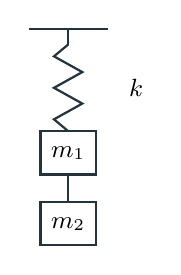
\begin{tikzpicture}
\draw[object] (-.5,3)--(.5,3);\draw[object] (0,3)--(0,2.8);
\draw[object] (0,2.8)--(-.18,2.65)--(.18,2.45)--(-.18,2.25)--(.18,2.05)--(-.18,1.85)--(0,1.7);
\filldraw[object,fill=white] (-.35,1.15) rectangle (.35,1.7);\node at (0,1.42) {$m_1$};\draw[object] (0,1.15)--(0,.8);\filldraw[object,fill=white] (-.35,.25) rectangle (.35,.8);\node at (0,.52) {$m_2$};\node[right] at (.65,2.25) {$k$};
\end{tikzpicture}
\figcaption{图 3.1\quad 撤去下挂物前的平衡状态。}
\end{minipage}\end{center}

\Needspace{5\baselineskip}\subsection*{解答}

以弹簧原长时 $m_1$ 的位置为原点，竖直向下为 $x$ 正方向。解图3.1A 上方的虚线是撤去下挂物后的平衡位置 $x_e$，下方的虚线是释放位置 $x_i$。物体从静止出发，两条线的距离就是这次振动的振幅。
\begin{center}\begin{minipage}{\linewidth}\centering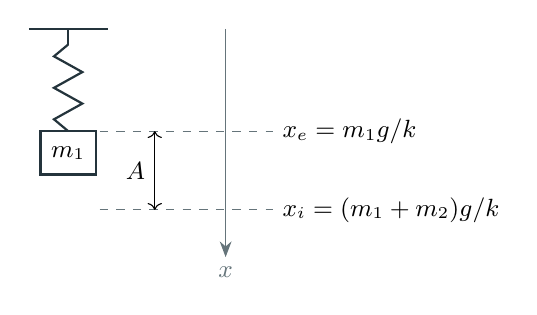
\begin{tikzpicture}
\draw[object] (-.5,3)--(.5,3);\draw[object] (0,3)--(0,2.8);
\draw[object] (0,2.8)--(-.18,2.65)--(.18,2.45)--(-.18,2.25)--(.18,2.05)--(-.18,1.85)--(0,1.7);
\filldraw[object,fill=white] (-.35,1.15) rectangle (.35,1.7);\node at (0,1.42) {$m_1$};\draw[axis] (2,3)--(2,.1) node[below] {$x$};\draw[guide] (.4,1.7)--(2.6,1.7);\draw[guide] (.4,.7)--(2.6,.7);
\node[right] at (2.6,1.7) {$x_e=m_1g/k$};\node[right] at (2.6,.7) {$x_i=(m_1+m_2)g/k$};\draw[<->] (1.1,.7)--(1.1,1.7) node[midway,left] {$A$};
\end{tikzpicture}
\figcaption{解图 3.1A\quad 从 $x_i$ 静止释放后，首次到 $x_e$ 时向上速率最大。}
\end{minipage}\end{center}

\subsubsection*{平衡位置与释放状态}
撤去下挂物之前，弹簧所承受的总重力为 $(m_1+m_2)g$，故伸长量
\[
x_i=\frac{(m_1+m_2)g}{k}.
\]
撤去过程不给冲量，所以撤去后的瞬间位置仍为 $x_i$，速度仍为零。此后参加运动的物体只有 $m_1$，新的平衡条件是 $kx_e=m_1g$，因而
\[
x_e=\frac{m_1g}{k},\qquad x_i-x_e=\frac{m_2g}{k}.
\]
解图 3.1A 中两条水平虚线之间的距离是相对新平衡位置的初位移。弹簧刚开始收缩时，弹力比 $m_1g$ 大 $m_2g$，所以 $m_1$ 先向上运动。

\subsubsection*{速度最大的位置}
撤去后的运动方程是 $m_1\ddot x=m_1g-kx$。令 $\xi=x-x_e$，便有
\[
\ddot\xi+\frac{k}{m_1}\xi=0.
\]
从 $x_i$ 上行到 $x_e$ 时，$\xi>0$，加速度向上，上行速率增加。越过 $x_e$ 后，$\xi<0$，加速度向下，上行速率减小。因而首次经过 $x_e$ 时速率最大。振动的最上端为 $x_e-A=(m_1-m_2)g/k$。$m_2\ge m_1$ 时物体能到弹簧原长处，那里弹力为零，加速度为向下的 $g$。

取物体、弹簧和地球为系统，势能可配方为
\[
U(x)=\frac12kx^2-m_1gx
=\frac12k(x-x_e)^2-\frac12kx_e^2.
\]
把释放位置代入同一势能式，可以把振动能量中的各项展开。初始速度为零，故释放瞬间的机械能为
\[
E=\frac12kx_i^2-m_1gx_i
=\frac{(m_1+m_2)^2g^2}{2k}
-\frac{m_1(m_1+m_2)g^2}{k}
=\frac{m_2^2-m_1^2}{2k}g^2,
\]
最小势能为 $U_{\min}=-m_1^2g^2/(2k)$。相减后留下 $m_2^2g^2/(2k)$，与配方中相对平衡位置的振动能量相同。
从释放点到新平衡位置，势能差全部转成动能：
\[
\frac12m_1v_{\max}^2
 =\frac12k(x_i-x_e)^2
 =\frac{m_2^2g^2}{2k}.
\]
所以
\[
\boxed{v_{\max}=\frac{m_2g}{\sqrt{m_1k}}}.
\]
简谐运动的角频率为 $\omega=\sqrt{k/m_1}$，速度幅值为 $\omega A$。从图3.1A 的 $x_i$ 到 $x_e$ 对应四分之一周期。当 $m_2\to0$ 时，两条平衡线靠拢，振幅和最大速率均趋零。
图3.1A 中实线方块在 $x_e$。第一次经过时速度为 $-v_{\max}$。由 $U'(x_e)=kx_e-m_1g=0$、$U''(x_e)=k>0$，也可看出这里是总势能唯一的最低点。撤去操作给出了 $x(0)=x_i,\dot x(0)=0$；此后的能量方程用留下的物体、弹簧和地球组成系统。


\Needspace{18\baselineskip}

\pdfbookmark[2]{第 2 题 带摩擦水平弹簧振子的过原点条件}{q2}

\section*{第 2 题\quad 带摩擦水平弹簧振子的过原点条件}

\tagline{M-03-02}

水平轻弹簧一端固定，另一端连接质量为 $m$ 的小球，劲度系数为 $k$。小球在粗糙水平面上运动，静、动摩擦系数均为 $\mu$。弹簧原长位置为 $O$。从右侧 $OA=l_0$ 的 $A$ 点静止释放。
\begin{enumerate}\item 为使小球穿过 $O$ 且只穿过一次，$\mu$ 应取什么范围？以速度不为零并越到另一侧为“穿过”。\item 若还要求小球在左侧第一个转折点 $B$ 永久停住，$OB=l_1$ 的最大值是多少？\end{enumerate}

\begin{center}\begin{minipage}{\linewidth}\centering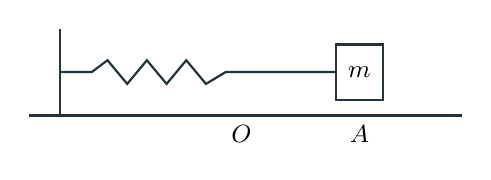
\begin{tikzpicture}
\draw[object] (-.4,0)--(5.1,0);\draw[object] (0,0)--(0,1.1);\draw[object] (0,.55)--(.4,.55)--(.6,.7)--(.85,.4)--(1.1,.7)--(1.35,.4)--(1.6,.7)--(1.85,.4)--(2.1,.55)--(3.5,.55);\filldraw[object,fill=white] (3.5,.2) rectangle (4.1,.9);\node at (3.8,.55) {$m$};\node[below] at (2.3,0) {$O$};\node[below] at (3.8,0) {$A$};
\end{tikzpicture}
\figcaption{图 3.2\quad 小球从伸长位置释放，摩擦始终反向于运动。}
\end{minipage}\end{center}

\Needspace{5\baselineskip}\subsection*{解答}

记 $d=\mu mg/k$，它是最大静摩擦能够平衡的弹簧伸长或压缩量。解图3.2A 中，球首次向左越过 $O$ 后在 $B$ 点停下。弹力若大于最大静摩擦，球便向右返回；若返回时动能先耗尽，它会在 $O$ 左侧再次停下。
\begin{center}\begin{minipage}{\linewidth}\centering\begin{tikzpicture}
\draw[axis] (-2.3,0)--(2.6,0) node[right] {$x$};\foreach \x/\lab in {-1.2/B,0/O,2/A}{\fill (\x,0) circle(2pt);\node[below] at (\x,0) {$\lab$};}
\draw[motion] (1.8,.5)--(-1,.5) node[midway,above] {第一次向左};\draw[motion] (-1,-.7)--(-.2,-.7) node[midway,below] {可能返回};\node at (-1.2,1.2) {$-l_1$};\node at (2,1.2) {$l_0$};
\end{tikzpicture}
\figcaption{解图 3.2A\quad 穿过原点与在首个转折点永久停住是两个条件。}
\end{minipage}\end{center}

\subsubsection*{首次穿过与左侧转折点}
设 $x$ 向右为正，并记 $d=\mu mg/k$。当 $kl_0\leq\mu mg$ 时，$A$ 点的弹力可以由静摩擦平衡，球保持静止。要从 $A$ 启动，需有 $l_0>d$，随后再根据到 $O$ 的动能判断是否穿过。
从 $A$ 向左到 $O$，摩擦力向右，所做的功为 $-\mu mgl_0$。到达 $O$ 的动能为
\[
K_O=\frac12kl_0^2-\mu mgl_0
 =\frac{k l_0}{2}(l_0-2d).
\]
“穿过”要求 $K_O>0$，即 $d<l_0/2$。这个条件也自动保证球能从 $A$ 开始运动。

设首次在左侧停下的位置为 $x=-l_1$，如解图 3.2A。此段总路程为 $l_0+l_1$，两端速度都为零，因此
\[
\frac12kl_0^2-\mu mg(l_0+l_1)=\frac12kl_1^2.
\]
分解平方差并约去正数 $l_0+l_1$，得到
\[
\boxed{l_1=l_0-2d}.
\]

\subsubsection*{转折后会不会再穿过}
在 $B$ 点，弹簧力向右，大小为 $kl_1$。若 $l_1\leq d$，静摩擦足以平衡弹力，小球永久留在 $B$。若 $l_1>d$，球向右运动，摩擦随之改向左。
后一种情况下，由 $B$ 返回 $O$ 的动能为
\[
K'_O=\frac12kl_1^2-\mu mgl_1
=\frac{k l_1}{2}(l_1-2d).
\]
只有 $l_1>2d$ 才能第二次穿过；$l_1=2d$ 时恰好停在 $O$；$d<l_1<2d$ 时在 $O$ 左侧停下。此时剩余压缩量 $2d-l_1<d$，静摩擦能将球留住，不会再开始新的往返。

所以“不再穿过”的统一条件是 $l_1\leq2d$，与首次穿过的条件联立：
\[
l_0-2d\leq2d,\qquad d<l_0/2.
\]
得
\[
\boxed{\frac{kl_0}{4mg}\leq\mu<\frac{kl_0}{2mg}}.
\]
取下界时，球返回到 $O$ 恰好速度为零，故只计第一次穿过。取上界时，首次到达 $O$ 就停下，穿过次数为零，因此上界是开端点。

\subsubsection*{首个转折点永久停住}
第二问要求第一次在 $B$ 停下后就保持静止，对应弹力 $kl_1$ 由最大为 $kd$ 的静摩擦平衡，即 $l_1\leq d$。代入 $d=(l_0-l_1)/2$，得 $3l_1\leq l_0$。于是
\[
\boxed{l_{1,\max}=\frac{l_0}{3}},\qquad
\boxed{\mu=\frac{kl_0}{3mg}}.
\]
整个一次穿过区间可以进一步分成两段：$l_0/4\leq d<l_0/3$ 时球会返回，但不再穿过；$l_0/3\leq d<l_0/2$ 时球留在第一个左侧转折点。
\subsubsection*{用往返路程计算摩擦耗能}
图3.2A 给出从 $A$ 到 $B$ 再返回的路线。能从 $B$ 启动时，沿这一路线累加摩擦功。
若小球从$B$启动返回，累计走到$O$的路程是$l_0+2l_1$，
这一路程所需的摩擦耗能为$\mu mg(l_0+2l_1)$。
不再穿过$O$要求候选返回动能不大于零，即
\[
\frac12kl_0^2-\mu mg(l_0+2l_1)\leq0.
\]
在已经确认返回会启动的分支中，这个不等式的等号表示恰好到$O$停住。
若球已留在$B$，这段返回路程并未发生，应使用前面的静摩擦判断；
它与上述分支最后给出同一个一次穿过区间。
代入$l_1=l_0-2\mu mg/k$，逐项整理为
\[
\begin{aligned}
&\frac{4m^2g^2}{k}\mu^2-3mgl_0\mu+\frac12kl_0^2\leq0,\\
&\frac{4m^2g^2}{k}
\left(\mu-\frac{kl_0}{4mg}\right)
\left(\mu-\frac{kl_0}{2mg}\right)\leq0.
\end{aligned}
\]
首项系数为正，故二次式在两根之间非正。
再与首次穿过所需的 $\mu<kl_0/(2mg)$ 相交，得到前面的左闭右开区间。左端对应返回到 $O$ 时动能为零，右端对应第一次到 $O$ 时动能为零，两个端点的运动不同。

返回却未过$O$时，还能求出最终位置。
记最终压缩量为$l_2\geq0$，从$B$到此处的路程是$l_1-l_2$，于是
\[
\frac12kl_1^2-\mu mg(l_1-l_2)=\frac12kl_2^2,
\qquad l_2=2d-l_1=4d-l_0.
\]
在$l_0/4\leq d<l_0/3$内，$0\leq l_2<d$，静摩擦能维持最后的停止。
球第二次停下的位置为 $x=-l_2$。由于 $l_2<l_1$，它已从第一次停下的位置 $x=-l_1$ 向右移动了一段。
解图3.2B用同一条$d/l_0$轴归纳各段过程：
能否启动、能否首次穿过、是否返回、返回后能否再穿过，需要按这个顺序判断。
\begin{center}\begin{minipage}{\linewidth}\centering
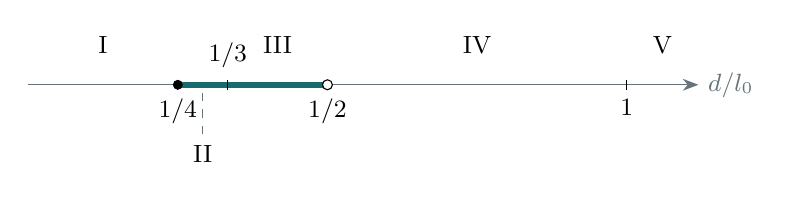
\begin{tikzpicture}[x=7.6cm]
\draw[axis] (0,0)--(1.12,0) node[right] {$d/l_0$};
\draw[traj,line width=2pt] (.25,0)--(.5,0);
\foreach \x/\lab in {.25/{1/4},.5/{1/2},1/{1}}{
 \draw (\x,-.06)--(\x,.06);\node[below] at (\x,-.06) {$\lab$};}
\draw (.333333,-.06)--(.333333,.06);\node[above] at (.333333,.09) {$1/3$};
\fill (.25,0) circle(1.8pt);\draw[fill=white] (.5,0) circle(1.8pt);
\node at (.125,.5) {I};\node at (.416667,.5) {III};
\node at (.75,.5) {IV};\node at (1.06,.5) {V};
\draw[guide] (.291667,-.1)--(.291667,-.65);\node[below] at (.291667,-.65) {II};
\end{tikzpicture}

\smallskip
\begin{tabular}{@{}cll@{}}
I & $0<d/l_0<1/4$ & 至少再次穿过\\
II & $1/4\leq d/l_0<1/3$ & 返回，但不再穿过\\
III & $1/3\leq d/l_0<1/2$ & 留在首个左转折点\\
IV & $1/2\leq d/l_0<1$ & 到不了左侧\\
V & $d/l_0\geq1$ & 可由静摩擦留在释放点
\end{tabular}
\figcaption{解图3.2B\quad 加粗区间为一次穿过；$d=0$时无摩擦，会持续往复穿过。}
\end{minipage}\end{center}


\Needspace{18\baselineskip}

\pdfbookmark[2]{第 3 题 斜面摩擦中动能等于势能的位置}{q3}

\section*{第 3 题\quad 斜面摩擦中动能等于势能的位置}

\tagline{M-03-03}

木块沿倾角 $\theta=30^\circ$ 的足够长斜面，以 $v_0=4.5\,\mathrm{m/s}$ 的初速度上滑。静、动摩擦系数均为 $\mu=0.35$。以初始位置为重力势能零点，求动能等于重力势能时相对初始位置的高度。取 $g=10\,\mathrm{m/s^2}$。

\begin{center}\begin{minipage}{\linewidth}\centering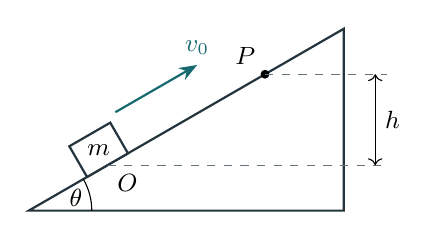
\begin{tikzpicture}
\draw[object] (0,0)--(4,2.309401)--(4,0)--cycle;
\filldraw[object,fill=white,rotate around={30:(1,.57735)}] (.7,.57735) rectangle (1.3,1.02735);
\node at (.8875,.772206) {$m$};\node[below right] at (1,.57735) {$O$};
\draw[motion] (1.1,1.25)--(2.13923,1.85) node[above] {$v_0$};
\draw (.8,0) arc(0:30:.8);\node at (.6,.16) {$\theta$};
\fill (3,1.732051) circle(1.6pt);\node[above left] at (3,1.732051) {$P$};
\draw[guide] (1,.57735)--(4.55,.57735);\draw[guide] (3,1.732051)--(4.55,1.732051);
\draw[<->] (4.4,.57735)--(4.4,1.732051) node[midway,right] {$h$};
\end{tikzpicture}
\figcaption{图 3.3\quad 从初始位置$O$量取竖直高度$h$，$P$表示上滑途中的位置。}
\end{minipage}\end{center}

\Needspace{5\baselineskip}\subsection*{解答}

解图3.3A 以初始点 $O$ 为高度零点。上滑从 $O$ 到 $h$，路程为 $h/\sin\theta$；下滑从最高点 $H$ 到 $h$，这段路程为 $(H-h)/\sin\theta$。两段中摩擦始终反向于运动，所做的功均为负。
\begin{center}\begin{minipage}{\linewidth}\centering\begin{tikzpicture}
\draw[axis] (0,-.2)--(0,3.2) node[above] {$h$};\foreach \y/\lab in {0/0,.8/h_2,1.7/h_1,2.7/H}{\draw (-.1,\y)--(.1,\y);\node[left] at (0,\y) {$\lab$};}\draw[motion] (1,.1)--(1,2.6) node[midway,right] {上滑};\draw[motion] (2.6,2.6)--(2.6,.1) node[midway,right] {下滑};\node[anchor=west,align=left] at (3.65,1.4) {$K_{\uparrow}=K_0-mg(1+\mu\cot\theta)h$\\$K_{\downarrow}=mg(1-\mu\cot\theta)(H-h)$};
\end{tikzpicture}
\figcaption{解图 3.3A\quad 同一高度处，上滑和下滑的动能不同。}
\end{minipage}\end{center}

\subsubsection*{上滑段}
设相对初始位置的竖直高度为 $h$，斜面路程为 $h/\sin\theta$。支持力为 $mg\cos\theta$，摩擦做功为
\[
W_f=-\mu mg\cos\theta\,\frac{h}{\sin\theta}
=-\mu mgh\cot\theta.
\]
记 $q=\mu\cot\theta$、$K_0=mv_0^2/2$。由动能定理，
\[
K_{\uparrow}(h)=K_0-mg(1+q)h.
\]
重力势能为 $U_g=mgh$，令两者相等，得到
\[
\boxed{h_1=\frac{v_0^2}{2g(2+q)}}.
\]
最高点由 $K_{\uparrow}(H)=0$ 确定，
\[
H=\frac{v_0^2}{2g(1+q)}.
\]
由于 $2+q>1+q$，可知 $0<h_1<H$，上滑过程中确实经过这一高度。

\subsubsection*{最高点能否返回}
木块停在最高点时，沿斜面向下的重力分量为 $mg\sin\theta$，最大静摩擦为 $\mu mg\cos\theta$。本题 $\mu=0.35<\tan30^\circ$，静摩擦不足以留住木块，所以还应计算下滑段。

从最高点下降至高度 $h$，路程为 $(H-h)/\sin\theta$。重力做正功、摩擦做负功，因而
\[
K_{\downarrow}(h)=mg(H-h)-\mu mg(H-h)\cot\theta
=mg(1-q)(H-h).
\]
令 $K_{\downarrow}(h_2)=mgh_2$，逐项移项：
\[
(1-q)H-(1-q)h_2=h_2,\qquad
\boxed{h_2=\frac{1-q}{2-q}H}.
\]

\subsubsection*{两个高度及其顺序}
$q=0.35\sqrt3\approx0.6062$，所以
\[
H\approx0.630\,\mathrm m,\quad
\boxed{h_1\approx0.388\,\mathrm m,\quad h_2\approx0.178\,\mathrm m}.
\]
解图3.3A 按 $0<h_2<h_1<H$ 标出两个位置。两次经过同一高度时，重力势能相同。下滑经过这一高度前，还走完了到最高点再返回的额外路程，因而动能较小；它与 $U_g=mgh$ 的交点也位于更低处。若改变摩擦系数，使木块在最高点由静摩擦保持静止，实际运动就结束在最高点，上滑时经过一次相等位置。
\subsubsection*{两段机械能的变化}
上滑段的功能关系可逐项写为
\[
-\mu mg\cos\theta\,\frac h{\sin\theta}
=\left(\frac12mv^2+mgh\right)-\frac12mv_0^2.
\]
代入$\frac12mv^2=mgh_1$后，
$\mu mgh_1\cot\theta=\frac12mv_0^2-2mgh_1$；
移项所得$2+q$中的$2$，分别对应相等的动能与重力势能，
$q$则对应这段上滑已经耗散的能量。
最高点的动能为零，同一关系给出
$\mu mgH\cot\theta=\frac12mv_0^2-mgH$。

下滑时以最高点为该段的初态，仍用初始位置$O$作重力势能零点，故
\[
\mu mg\cos\theta\frac{H-h_2}{\sin\theta}
=mgH-\left(mgh_2+\frac12mv_2^2\right).
\]
代入 $\frac12mv_2^2=mgh_2$，得到 $q(H-h_2)=H-2h_2$。下降释放的重力势能为 $mg(H-h_2)$，其中 $q\,mg(H-h_2)$ 被摩擦耗散，剩下 $(1-q)mg(H-h_2)$ 成为动能。
解图3.3B把这三个能量函数画在同一坐标中，两个交点分别落在上滑和下滑支上。
\begin{center}\begin{minipage}{\linewidth}\centering
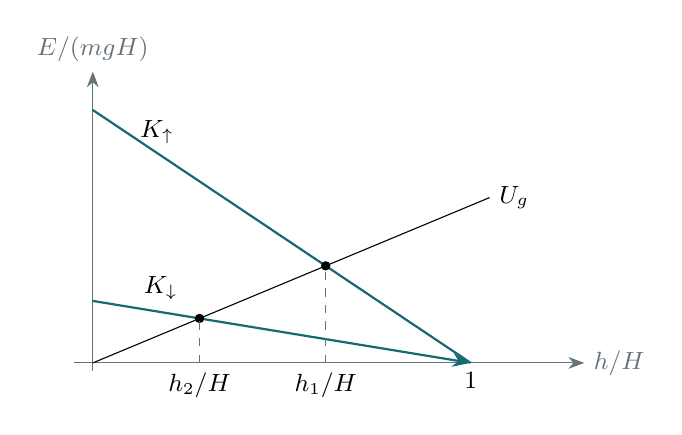
\begin{tikzpicture}[x=4.8cm,y=2cm]
\draw[axis] (-.05,0)--(1.3,0) node[right] {$h/H$};
\draw[axis] (0,-.05)--(0,1.85) node[above] {$E/(mgH)$};
\draw[traj,domain=0:1] plot(\x,{1.606218*(1-\x)});
\draw[motion,domain=0:1] plot(\x,{.393782*(1-\x)});
\draw[thin,domain=0:1.05] plot(\x,\x);
\node[above] at (.17,1.33) {$K_{\uparrow}$};
\node[above] at (.18,.34) {$K_{\downarrow}$};
\node[right] at (1.05,1.05) {$U_g$};
\fill (.616303,.616303) circle(1.7pt);\fill (.282528,.282528) circle(1.7pt);
\draw[guide] (.616303,0)--(.616303,.616303);
\draw[guide] (.282528,0)--(.282528,.282528);
\node[below] at (.616303,0) {$h_1/H$};\node[below] at (.282528,0) {$h_2/H$};
\node[below] at (1,0) {$1$};
\end{tikzpicture}
\figcaption{解图3.3B\quad 取$q=0.35\sqrt3$；两动能曲线在最高点归零，在不同位置与$U_g$相交。}
\end{minipage}\end{center}
两段都经过同一高度$h$时，两次动能相差
$K_{\uparrow}-K_{\downarrow}=2\mu mg(H-h)\cot\theta$。
这正是往返最高点所增加的两段路程的摩擦耗能；
当$\mu\to0$时差值消失，两次相等出现在同一高度$H/2$，但发生在不同的时刻。


\Needspace{18\baselineskip}

\pdfbookmark[2]{第 4 题 桌孔下落绳的速度与位置}{q4}

\section*{第 4 题\quad 桌孔下落绳的速度与位置}

\tagline{M-03-04}

均匀柔软、不可伸长的绳全长为 $l$，一部分平放在光滑水平桌面上，另一部分经过光滑小孔竖直下垂。初始下垂长度 $0<x_0<l$，整绳从静止下落。设桌上绳已经理顺，各段速率相同，小孔只改变运动方向。求绳速 $v(x)$ 及下端位置 $x(t)$，并说明适用时间。

\begin{center}\begin{minipage}{\linewidth}\centering\begin{tikzpicture}
\draw[object] (-2,1.6)--(-.12,1.6);\draw[object] (.12,1.6)--(1.7,1.6);\draw[traj] (-1.8,1.6)--(0,1.6)--(0,-.8);\node[above right] at (.15,1.6) {$O$};\draw[<->] (.7,-.8)--(.7,1.6) node[midway,right] {$x$};
\end{tikzpicture}
\figcaption{图 3.4\quad 向下量取下垂长度。}
\end{minipage}\end{center}

\Needspace{5\baselineskip}\subsection*{解答}

解图3.4A 中，绳从桌面经过小孔转向下落。整根绳是同一批物质，各段速率相同，以下把全长 $l$、线密度 $\lambda$ 的绳作为系统。桌上部分与下垂部分都计入动能。
\begin{center}\begin{minipage}{\linewidth}\centering\begin{tikzpicture}
\draw[object] (-2,1.6)--(-.12,1.6);\draw[object] (.12,1.6)--(1.7,1.6);\draw[traj] (-1.8,1.6)--(0,1.6)--(0,-.8);\node[above right] at (.15,1.6) {$O$};\draw[<->] (.7,-.8)--(.7,1.6) node[midway,right] {$x$};\fill (0,.4) circle(2pt);\node[left] at (0,.4) {下垂段重心};\node[align=left] at (4,.7) {$K=\tfrac12\lambda l v^2$\\$U=-\tfrac12\lambda gx^2$};
\end{tikzpicture}
\figcaption{解图 3.4A\quad 下垂部分的重心深度为 $x/2$，动能按全绳质量计算。}
\end{minipage}\end{center}

\subsubsection*{整绳的动能和势能}
线密度记为 $\lambda$。绳不可伸长，且桌上部分已经理顺，各段速率同为 $v$，故整绳动能是
\[
K=\frac12\lambda l v^2.
\]
其中 $\lambda x$ 的下垂段沿竖直方向运动，$\lambda(l-x)$ 的桌上段沿水平方向运动，两部分速率相同，动能相加的质量系数为 $\lambda l$。

以下垂方向为正，从桌面向下取微元坐标 $y$。每个微元的重力势能为 $-g y\,\lambda\dd y$，故
\[
U=\int_0^x-\lambda gy\,\dd y=-\frac12\lambda gx^2.
\]
解图 3.4A 的下垂段重心深度为 $x/2$，用 $U=-(\lambda x)g(x/2)$ 也得到同一式子。桌上部分高度为零，无重力势能。

\subsubsection*{速率随位置的变化}
桌面与小孔光滑，只改变绳的方向，约束力不做功。整绳质量固定，能量守恒给出
\[
\frac12\lambda l v^2-\frac12\lambda gx^2
=-\frac12\lambda gx_0^2.
\]
约去 $\lambda/2$ 后，
\[
\boxed{v(x)=\sqrt{\frac gl(x^2-x_0^2)}}.
\]
取正根，因为这一阶段下垂长度单调增加。$x=x_0$ 时速率为零，符合初始条件；$x$ 越大，下垂重力越大，速率也越大。

\subsubsection*{时间积分与接续}
利用 $v=\dot x$，分离变量：
\[
\int_{x_0}^{x}\frac{\dd\xi}{\sqrt{\xi^2-x_0^2}}
=\sqrt{\frac gl}\,t.
\]
令 $\xi=x_0\cosh u$，积分左端等于 $\operatorname{arcosh}(x/x_0)$，得到
\[
\boxed{x(t)=x_0\cosh\!\left(\sqrt{\frac gl}\,t\right)}.
\]
对位置式求导，得到 $\dot x=x_0\sqrt{g/l}\sinh(\sqrt{g/l}\,t)$、$\ddot x=gx/l$。初始速度为零，初始加速度为 $gx_0/l$，它等于下垂段重力 $\lambda gx_0$ 除以全绳质量 $\lambda l$。

绳全部离桌时 $x=l$，对应
\[
t_*=\sqrt{\frac lg}\operatorname{arcosh}\frac l{x_0},\qquad
v_*=\sqrt{\frac gl(l^2-x_0^2)}.
\]
双曲余弦公式只适用于 $0\leq t\leq t_*$。之后整绳自由下落，下端位置应接为
\[
x=l+v_*(t-t_*)+\frac12g(t-t_*)^2.
\]
位置与速度在接续点连续；加速度也由 $gx/l$ 在 $x=l$ 时达到 $g$。
\subsubsection*{沿绳的切向动力学与积分常数}
将整绳分成小段，对每段沿运动方向写切向方程，可以求出牵动全绳的力。
各段的切向加速度都等于$\dot v$；相邻小段的张力在求和时抵消，
光滑孔口的法向约束力不进入切向方程。
于是质量系数为整绳质量$m=\lambda l$，驱动项为下垂段重力$\lambda gx$，即
\[
\lambda l\,\dot v=\lambda gx.
\]
各小段的投影方向随绳走向而变，这条标量式把它们的切向分量相加。桌上段水平运动，下垂段竖直运动；小孔对经过孔口的绳提供法向作用，使速度矢量转向，同时保持速率连续。
由$\dot v=v\,\dd v/\dd x$，有
\[
v\,\dd v=\frac glx\,\dd x,
\qquad v^2=\frac glx^2+C.
\]
初值$x=x_0,v=0$确定$C=-gx_0^2/l$，再选下落的正根，得到前面的$v(x)$。

时间积分中的代换也可展开。令$\xi=x_0\cosh u$，
则$\dd\xi=x_0\sinh u\,\dd u$且$\sqrt{\xi^2-x_0^2}=x_0\sinh u$，
两者约去后积分等于$u$。不定积分的完整形式为
\[
\operatorname{arcosh}(x/x_0)=\sqrt{g/l}\,t+C_t.
\]
$t=0$时$x=x_0$，左端为零，所以$C_t=0$。
解图3.4A 的 $x$ 从孔口量到绳下端，故全绳各段的速率为 $\dot x$。下垂段一面运动，一面纳入从桌面转来的绳元，所以 $x/2$ 表示每一时刻下垂部分的重心深度。它用于求当时的重力势能，全绳动能则按每段的速率 $\dot x$ 相加。


\Needspace{18\baselineskip}

\pdfbookmark[2]{第 5 题 单摆碰钉后的完整圆周与撞钉条件}{q5}

\section*{第 5 题\quad 单摆碰钉后的完整圆周与撞钉条件}

\tagline{M-03-05}

摆长为 $L$ 的单摆，从悬点 $O$ 左侧、与向下竖直方向夹角 $\alpha$ 处静止释放。右侧钉子 $P$ 满足 $OP=r<L$，$OP$ 与向下竖直方向夹角为 $\beta$，其中 $0<\beta<\alpha\leq90^\circ$。绳转到 $OP$ 方向后绕钉运动，绳与钉均理想光滑。求：\begin{enumerate}\item 完成绕钉圆周运动的最小释放角；\item 绳松弛后，小球沿抛物线直接击中钉子 $P$ 所需的释放角。若条件不能实现，应说明。\end{enumerate}

\begin{center}\begin{minipage}{\linewidth}\centering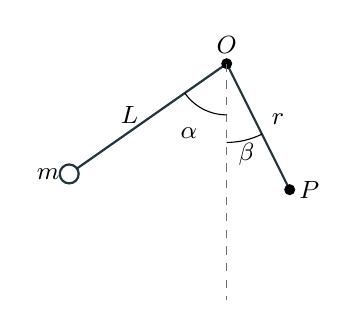
\begin{tikzpicture}
\coordinate(O)at(0,3);\coordinate(P)at(.8,1.4);\coordinate(A)at(-2,1.6);\draw[object] (A)--(O)--(.8,1.4);\fill(O)circle(2pt);\fill(P)circle(2pt);\filldraw[object,fill=white](A)circle(.12);\draw[guide](O)--(0,0);\node[above]at(O){$O$};\node[right]at(P){$P$};\node[left]at(A){$m$};\node[left]at(-1,2.35){$L$};\node[right]at(.45,2.3){$r$};\draw (0,2.35) arc(-90:-145:.65);\node at(-.48,2.12){$\alpha$};\draw (0,2) arc(-90:-63.435:1);\node at(.25,1.85){$\beta$};
\end{tikzpicture}
\figcaption{图 3.5\quad 绳碰钉后，运动半径变为 $a=L-r$。}
\end{minipage}\end{center}

\Needspace{5\baselineskip}\subsection*{解答}

令 $a=L-r$，以钉子为圆心，$\theta$ 从向下竖直方向量起，如解图 3.5A。球的高度为 $-r\cos\beta-a\cos\theta$（相对 $O$）。
\begin{center}\begin{minipage}{\linewidth}\centering\begin{tikzpicture}
\coordinate(P)at(0,0);\draw[guide](P)circle(1.5);\draw[guide](P)--(0,-1.8);\draw[object](P)--(1.15, .96);\fill(P)circle(2pt);\filldraw[object,fill=white](1.15,.96)circle(.1);\draw[motion](1.15,.96)--(.55,1.68)node[above]{$v$};\draw[force](1.15,.96)--(1.15,.2)node[right]{$mg$};
\draw[force](1.15,.96)--(.575,.48)node[below left]{$T$};\node[left]at(P){$P$};\node[right]at(.65,.4){$a$};\draw (0,-.55) arc(-90:40:.55);\node at(.7,-.3){$\theta$};\node[align=left]at(4,0){$T=mv^2/a+mg\cos\theta$\\松绳处：$T=0$};
\end{tikzpicture}
\figcaption{解图 3.5A\quad 完整圆周的临界状态在最高点确定；撞钉轨道由松绳点接续抛体运动。}
\end{minipage}\end{center}

\subsubsection*{碰钉后的能量与张力}
球绕钉后的半径为 $a=L-r$。相对悬点 $O$，释放点高度为 $-L\cos\alpha$；绕钉位置的高度为 $-r\cos\beta-a\cos\theta$，如解图 3.5A。理想光滑钉不耗能，故
\[
\frac12mv^2=mg(r\cos\beta+a\cos\theta-L\cos\alpha).
\]
取指向 $P$ 为径向正向，张力与重力分量满足
\[
T-mg\cos\theta=\frac{mv^2}{a}.
\]
因此
\[
v^2=2g(r\cos\beta+a\cos\theta-L\cos\alpha),
\]
\[
T=3mg\cos\theta+\frac{2mg}{a}(r\cos\beta-L\cos\alpha).
\]
圆周上的每个位置都需有实速率 $v^2\geq0$；绳力沿半径向内，张紧状态还需 $T\geq0$。在 $\pi/2<\theta<\pi$ 的上行段，$\mathrm dT/\mathrm d\theta=-3mg\sin\theta<0$。若这一段上 $T$ 降到零，沿圆弧继续上行将要求绳沿半径向外推，小球便从该点沿切线进入自由飞行。完整圆周的临界情形在最高点取到张力的零最小值，过最高点后张力重新增大。

\subsubsection*{完整圆周的临界释放角}
在绕钉的上行段，$\cos\theta$ 逐渐减小，张力最低的位置是最高点 $\theta=\pi$。临界时 $T_{\mathrm{top}}=0$。最高点的重力全部用于圆周向心加速度，故 $v_{\mathrm{top}}^2=ga$，速度水平，方向沿圆的切线。
代入张力式，
\[
-3mg+\frac{2mg}{a}(r\cos\beta-L\cos\alpha)=0.
\]
记
\[
C_1=\frac rL\cos\beta-\frac{3a}{2L},
\]
则完整圆周要求 $\cos\alpha\leq C_1$。在 $0<\alpha\leq90^\circ$ 内，余弦随释放角增大而减小，所以
\[
\boxed{\alpha_{\min}=\arccos C_1}.
\]
题设 $\beta<\alpha\leq90^\circ$，即 $0\leq\cos\alpha<\cos\beta$。因此可实现条件是 $C_1\geq0$；当它等于零时，恰从水平位置 $\alpha=90^\circ$ 释放。又因 $C_1<\cos\beta$，可实现时自动有 $\alpha_{\min}>\beta$。

\subsubsection*{松绳后直接击中钉子}
\begin{center}\begin{minipage}{\linewidth}\centering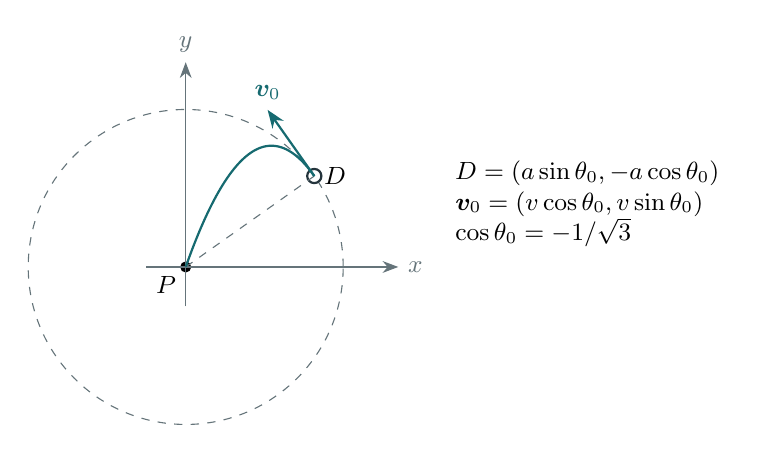
\begin{tikzpicture}
\draw[guide](0,0)circle(2);
\coordinate(P)at(0,0);\coordinate(D)at(1.633,1.155);
\fill(P)circle(2pt);\filldraw[object,fill=white](D)circle(.09);
\draw[guide](P)--(D);\draw[axis](-.5,0)--(2.7,0)node[right]{$x$};
\draw[axis](0,-.5)--(0,2.6)node[above]{$y$};
\draw[traj,domain=0:1,samples=60]plot({1.633*(1-\x)},{1.155+2.309*\x-3.464*\x^2});
\draw[motion](D)--(1.04,1.995)node[above]{$\vect v_0$};
\node[below left]at(P){$P$};\node[right]at(D){$D$};
\node[align=left]at(5.1,.8){$D=(a\sin\theta_0,-a\cos\theta_0)$\\
$\vect v_0=(v\cos\theta_0,v\sin\theta_0)$\\$\cos\theta_0=-1/\sqrt3$};
\end{tikzpicture}
\figcaption{解图 3.5B\quad 松绳后的抛物线直接经过钉子；虚圆是此前的圆周轨道。}
\end{minipage}\end{center}
如解图 3.5B，设松绳点的角度为 $\theta_0\in(\pi/2,\pi)$。由 $T=0$，
\[
v^2=-ag\cos\theta_0.
\]
以 $P$ 为原点，水平向右、竖直向上，松绳位置和速度为
\[
(x_0,y_0)=(a\sin\theta_0,-a\cos\theta_0),\quad
(v_x,v_y)=(v\cos\theta_0,v\sin\theta_0).
\]
飞行时间记为 $\tau$。命中原点要求
\[
0=a\sin\theta_0+v\cos\theta_0\,\tau,\qquad
0=-a\cos\theta_0+v\sin\theta_0\,\tau-\frac12g\tau^2.
\]
第一式给出 $\tau=-a\sin\theta_0/(v\cos\theta_0)>0$。代入第二式并利用 $\sin^2\theta_0+\cos^2\theta_0=1$，得
\[
v^2=-\frac{ag\sin^2\theta_0}{2\cos\theta_0}.
\]
与松绳条件联立，得到 $2\cos^2\theta_0=\sin^2\theta_0$。根据所在象限取
\[
\cos\theta_0=-\frac1{\sqrt3},\qquad
\theta_0\approx125.26^\circ.
\]
再由张力式求释放角：
\[
\boxed{\alpha=\arccos\!\left(\frac rL\cos\beta-
\frac{\sqrt3a}{2L}\right)}.
\]
括号内须非负，才能使 $\alpha\leq90^\circ$；它也小于 $\cos\beta$，故 $\alpha>\beta$ 自动成立。这一释放角确定球在 $\theta_0$ 第一次松绳，速度方向由图3.5B 的圆弧切线给出，之后的抛物线通过 $P$。
\subsubsection*{松绳后的抛体是否会被绳再次拉住}
命中条件还要与绳长相容。以解图3.5B中的$D$为起点，
记从$D$飞到$P$的时间为$\tau_P$。
水平命中式与$\cos\theta_0=-1/\sqrt3$给出
\[
\tau_P=\frac{\sqrt2a}{v},\qquad
v^2=\frac{ag}{\sqrt3},\qquad
\tau_P^2=\frac{2\sqrt3a}{g}.
\]
令$u=\tau/\tau_P$，把速度、时间代入抛体坐标，得到
\[
\frac xa=\sqrt{\frac23}(1-u),\qquad
\frac ya=\frac{1+2u-3u^2}{\sqrt3},\qquad 0\leq u\leq1.
\]
图3.5B 中 $D$ 是固定的松绳点。飞行中的小球到钉子的距离记为 $d_P(\tau)$，满足
\[
\frac{d_P^2(\tau)}{a^2}
=\frac23(1-u)^2+\frac13(1+2u-3u^2)^2
=1-4u^3+3u^4\leq1.
\]
在$0<u<1$内，$u^3(3u-4)<0$，小球始终处在半径$a$的圆内，
绳不会在命中前再次张紧。即使松绳后与钉子的接触方式改变，
由三角不等式，悬点到球的直线距离也不超过$r+d_P<L$，同样不会提前拉紧。
解图3.5B中圆弧之后的实线抛物线因此是可以实际经过的自由飞行段。

碰钉前后的张力随运动位置有如下变化。在碰钉前的长摆段，若位置角为$\psi$，
则$T_O=mg(3\cos\psi-2\cos\alpha)\geq mg\cos\alpha\geq0$。
碰钉后，从$\theta=\beta$到$\theta_0$，
$T(\theta)$随$\cos\theta$减少而下降，第一次到零正是上面求出的松绳点，
不会在到达$D$前就失去圆周约束。
完整圆周的临界条件还给出$v_{\mathrm{top}}^2=ga>0$，
其余位置的高度更低、速率更大，张力也更大，故最高点达到临界时整圈均满足张紧条件。


\Needspace{18\baselineskip}

\pdfbookmark[2]{第 6 题 圆环双球下滑与悬线张力}{q6}

\section*{第 6 题\quad 圆环双球下滑与悬线张力}

\tagline{M-03-06}

质量 $M$、半径 $R$ 的竖直圆环，用轻细线悬挂。环上串着两个质量均为 $m$ 的光滑小球，从顶端以无限小扰动同时向两侧滑下。$\theta$ 从向上竖直半径量起。\begin{enumerate}\item 假设圆环不动，画出悬线张力 $T$ 随 $x=\cos\theta$ 的曲线，求最小值及对应角度。\item 求圆环可能上升的质量比阈值，画出阈值情形的曲线，并区分“张力为零”与“实际上升”。\end{enumerate}

\begin{center}\begin{minipage}{\linewidth}\centering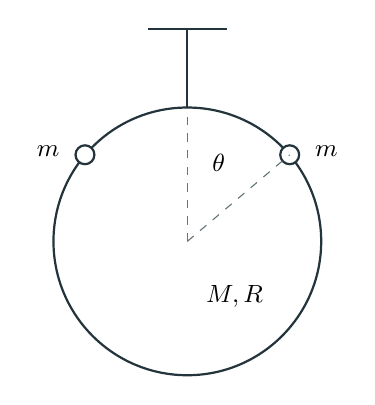
\begin{tikzpicture}
\draw[object](0,0)circle(1.7);\draw[object](0,1.7)--(0,2.7);\draw[object](-.5,2.7)--(.5,2.7);\filldraw[object,fill=white](1.3,1.1)circle(.12);\filldraw[object,fill=white](-1.3,1.1)circle(.12);\draw[guide](0,0)--(0,1.7);\draw[guide](0,0)--(1.3,1.1);\node at(.4,1){$\theta$};\node[right]at(1.5,1.15){$m$};\node[left]at(-1.5,1.15){$m$};\node at(.6,-.7){$M,R$};
\end{tikzpicture}
\figcaption{图 3.6\quad 小球串在环上，可承受环沿径向的推、拉作用。}
\end{minipage}\end{center}

\Needspace{5\baselineskip}\subsection*{解答}

小球的速度满足 $v^2=2gR(1-\cos\theta)$。取小球所受环力 $N$ 以沿半径向外为正，径向方程给出 $N=mg(3\cos\theta-2)$。解图 3.6A 的曲线采用阈值质量比。
\begin{center}\begin{minipage}{\linewidth}\centering\begin{tikzpicture}
\draw[axis](-2.2,0)--(2.2,0)node[right]{$x$};\draw[axis](0,-.2)--(0,3.4)node[above]{$T/(Mg)$};\draw[traj,domain=-1:1,samples=80]plot({2*\x},{.18*(3*\x-1)^2});\draw[guide](.6667,0)--(.6667,.6);\node[below]at(.6667,0){$1/3$};\node[below]at(-2,0){$-1$};\node[below]at(2,0){$1$};\node[left]at(0,.18){$1$};\node[align=left]at(5,1.8){阈值 $m/M=3/2$\\$T/(Mg)=(3x-1)^2$\\曲线在 $x=1/3$ 与横轴相切};
\end{tikzpicture}
\figcaption{解图 3.6A\quad 阈值时只触及零张力，没有一段需要负张力的区域。}
\end{minipage}\end{center}

\subsubsection*{先按圆环固定计算反力}
每球从环顶下降的高度为 $R(1-\cos\theta)$，由能量守恒，
\[
v^2=2gR(1-\cos\theta).
\]
小球串在环上，环既能将它向外推，也能向内拉。设环对球的径向作用力 $N$ 以向外为正。向外方向的重力分量为 $-mg\cos\theta$，向外加速度为 $-v^2/R$，故
\[
N-mg\cos\theta=-\frac{mv^2}{R},\qquad
N=mg(3\cos\theta-2).
\]
当 $N<0$，环对串珠的作用力沿半径向内。串珠套在环上，仍沿圆弧运动，图3.6B 中对环的反作用力随之改向。

\begin{center}\begin{minipage}{\linewidth}\centering\begin{tikzpicture}
\draw[guide](0,0)circle(1.65);
\filldraw[object,fill=white](1,1.312)circle(.09);
\draw[guide](0,0)--(1,1.312);\draw[force](1,1.312)--(1.48,1.94)node[right]{$N$};
\draw[force](1,1.312)--(1,.35)node[right]{$mg$};
\node at(0,-2){单球受力};
\draw[object](5,0)circle(1.65);\draw[object](5,1.65)--(5,2.2);
\draw[force](5,2.2)--(5,3.1)node[right]{$T$};
\draw[force](5,0)--(5,-.9)node[right]{$Mg$};
\draw[force](4,1.312)--(4.45,.72)node[left]{$-N$};
\draw[force](6,1.312)--(5.55,.72)node[right]{$-N$};
\node at(5,-2){圆环受力};
\end{tikzpicture}
\figcaption{解图 3.6B\quad 球与环的作用力、反作用力分开画；$N$ 按外径正向取有符号值。}
\end{minipage}\end{center}
解图 3.6B 中，球对环的反作用力为 $-N$ 沿半径，其竖直分量为 $-N\cos\theta$。两球的水平分量相互抵消。圆环不动时，竖直平衡为
\[
T-Mg-2N\cos\theta=0.
\]
令 $x=\cos\theta$，得
\[
\boxed{T(x)=Mg+2mg(3x^2-2x)},\quad -1\leq x\leq1.
\]

\subsubsection*{抛物线的顶点与阈值}
以抛物线的顶点配方：
\[
T(x)=6mg\left(x-\frac13\right)^2+Mg-\frac23mg.
\]
所以
\[
\boxed{T_{\min}=Mg-\frac23mg},\quad
\boxed{\theta_{\min}=\arccos(1/3)\approx70.53^\circ}.
\]
运动时 $x$ 从 $1$ 向 $-1$ 变化，曲线先降后升。若 $m/M<3/2$，最低值仍为正，悬线可始终维持环不动。

当 $m/M=3/2$ 时，解图 3.6A 给出
\[
\boxed{\frac{T}{Mg}=(3x-1)^2}.
\]
曲线只在 $x=1/3$ 与零线相切。在这一瞬间，悬线张力为零。顶点两侧的所需张力均为正，因此曲线在整个运动区间仍能由向上的悬线力实现。阈值质量比对应的是一瞬间的零张力。

\subsubsection*{实际开始上升的位置}
若 $m/M>3/2$，假设固定的计算会出现 $T<0$。此时保持环固定需要向下的力，悬线所能给出的拉力却只能向上，所以圆环转入悬线松弛后的运动。求 $T=0$ 的两根：
\[
x_\pm=\frac{1\pm\sqrt{1-3M/(2m)}}3.
\]
因为小球运动时 $x$ 从 $1$ 下降，先遇到较大根，故
\[
\boxed{\theta_{\mathrm{lift}}=\arccos x_+},\qquad
\boxed{\frac mM>\frac32\text{ 时可实际上升}}.
\]
环开始运动后，球与环之间有能量、动量交换，以上“环固定”的速度和张力函数只用到约束失效的一刻。顶端的静止状态本身为不稳定平衡，本题释放理解为给无限小扰动再取极限。
\subsubsection*{函数取值、判别式与可实现的曲线段}
若用求导法，
\[
\frac{\dd T}{\dd x}=12mgx-4mg=0
\quad\Longrightarrow\quad x=\frac13,
\qquad\frac{\dd^2T}{\dd x^2}=12mg>0.
\]
顶点在实际范围$[-1,1]$内，所以给出的确是整个固定环模型的最小张力。
从环顶、水平侧点到环底，分别代入 $x=1,0,-1$，可读出
\begin{center}
\begin{tabular}{@{}rrrrrr@{}}\toprule
$x=\cos\theta$ & $-1$ & $0$ & $1/3$ & $2/3$ & $1$\\\midrule
$T$ & $Mg+10mg$ & $Mg$ & $Mg-2mg/3$ & $Mg$ & $Mg+2mg$\\
$m/M=3/2$时$T/(Mg)$ & 16 & 1 & 0 & 1 & 4\\\bottomrule
\end{tabular}
\end{center}
从环顶到环底，读表方向是$x=1$到$x=-1$，与横轴数值增加的方向相反。
解图3.6C在同一坐标中比较三种质量比，便于区分最低张力为正、相切与出现负值三种情形。
\begin{center}\begin{minipage}{\linewidth}\centering
\begin{tikzpicture}
\draw[axis] (-2.25,0)--(2.3,0) node[right] {$x$};
\draw[axis] (0,-.32)--(0,3.2) node[above] {$T/(Mg)$};
\foreach \x/\lab in {-2/{-1},.666667/{1/3},2/{1}}{\draw (\x,-.04)--(\x,.04);\node[below] at (\x,-.04) {$\lab$};}
\foreach \y/\lab in {.14/1,1.4/10,2.8/20}{\draw (-.04,\y)--(.04,\y);\node[left] at (-.04,\y) {$\lab$};}
\draw[thin,domain=-1:1,samples=100] plot({2*\x},{.14*(1+2*(3*(\x)^2-2*\x))});
\draw[traj,domain=-1:1,samples=100] plot({2*\x},{.14*(3*\x-1)^2});
\draw[force,dashed,domain=-1:.5,samples=100] plot({2*\x},{.14*(1+4*(3*(\x)^2-2*\x))});
\draw[force,domain=.5:1,samples=50] plot({2*\x},{.14*(1+4*(3*\x^2-2*\x))});
\fill (1,0) circle(1.8pt);\draw[guide] (1,.04)--(1,.7);\node[above] at (1.2,.8) {$x_+=1/2$};
\draw[thin] (3,2.8)--(3.65,2.8) node[right] {$m/M=1$};
\draw[traj] (3,2.25)--(3.65,2.25) node[right] {$m/M=3/2$};
\draw[force] (3,1.7)--(3.65,1.7) node[right] {$m/M=2$};
\node[align=left,anchor=north west] at (3,1.35) {曲线均按环固定求得\\$m/M=2$时仅$x\geq1/2$\\属于实际固定环阶段\\虚线为失效后的形式延拓};
\end{tikzpicture}
\figcaption{解图3.6C\quad 不同质量比下保持圆环固定所需的张力；质量比超过阈值时，实线止于首次松弛点，虚线给出固定环的形式延拓。}
\end{minipage}\end{center}

从圆环受力也能推出相同阈值。悬线松弛时，
小球作用于环的向上合力必须至少抵消$Mg$，故
\[
-2N\cos\theta\geq Mg,
\qquad 3x^2-2x+\frac{M}{2m}\leq0.
\]
这个开口向上的二次式要存在非正值，必须有
\[
\Delta=4-4\cdot3\cdot\frac{M}{2m}
=4-\frac{6M}{m}\geq0,
\qquad\frac mM\geq\frac32.
\]
等号只给一个零点，严格大于才给两个不同零点及其间的负张力需求。
圆环刚离开固定位置时，记环心的向上位移为 $Y$，球相对圆环的切向速率为 $v$。球的向外径向加速度是 $\ddot Yx-v^2/R$，所以环对每球的作用为 $N=m(g+\ddot Y)x-mv^2/R$。与圆环的竖直方程联立，
\[
(M+2mx^2)\ddot Y=T-Mg-2m(gx-v^2/R)x.
\]
在图3.6C 的首次零点，$T=0$，右侧等于零，$\ddot Y=0$。紧接着 $x$ 继续减小，右侧从零开始增大：在离位瞬间 $v$ 的变化率仍与固定环时相同，因而右侧的时间导数等于图中有符号固定环张力的负时间导数。分母 $M+2mx^2>0$，所以环开始向上。曲线虚线段只给出保持圆环固定所需的外力；环抬起时悬线张力取零。


\Needspace{18\baselineskip}

\pdfbookmark[2]{第 7 题 滑杆脱离约束后的落点}{q7}

\section*{第 7 题\quad 滑杆脱离约束后的落点}

\tagline{M-03-07}

长 $2r=20\,\mathrm{cm}$ 的理想轻杆，在中心 $C$ 固定质量为 $m$ 的质点。端点 $A$ 靠在光滑竖直墙上，端点 $B$ 支在光滑水平地面上。杆从近似竖直的位置由静止下滑，运动始终在同一竖直平面。按集中质量轻杆模型，求中心 $C$ 第一次触地时距墙角 $O$ 的水平距离。

\begin{center}\begin{minipage}{\linewidth}\centering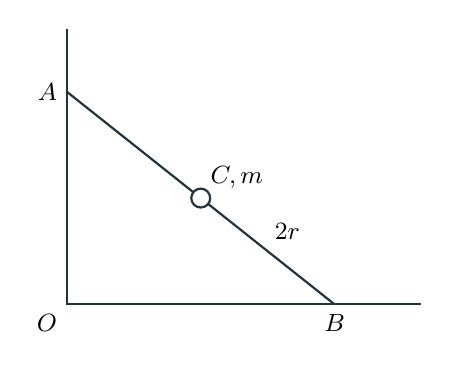
\begin{tikzpicture}
\draw[object](0,3.5)--(0,0)--(4.5,0);\draw[object](0,2.7)--(3.4,0);\filldraw[object,fill=white](1.7,1.35)circle(.12);\node[left]at(0,2.7){$A$};\node[below]at(3.4,0){$B$};\node[above right]at(1.7,1.35){$C,m$};\node[below left]at(0,0){$O$};\node[above]at(2.8,.7){$2r$};
\end{tikzpicture}
\figcaption{图 3.7\quad 两端保持接触时，杆中心沿半径 $r$ 的四分之一圆运动。}
\end{minipage}\end{center}

\Needspace{5\baselineskip}\subsection*{解答}

两端均接触时，$C=(r\sin\theta,r\cos\theta)$，其中 $\theta$ 从竖直方向量起。轻杆对 $C$ 的转动惯量为零，端点支持力的合力沿 $OC$，故中心运动等效于从圆弧外侧滑落。
\begin{center}\begin{minipage}{\linewidth}\centering\begin{tikzpicture}
\draw[axis](0,0)--(4,0)node[right]{$x$};\draw[axis](0,0)--(0,3)node[above]{$y$};\draw[guide](0,2.4)arc(90:0:2.4);\coordinate(D)at(1.789,1.6);\fill(D)circle(2pt);\draw[object](0,0)--(D);\draw[motion](D)--(2.4,.917)node[right]{$v_d$};\draw[traj,domain=0:1,samples=40]plot({1.789+.910*\x},{1.6-1.018*\x-.582*\x^2});\node[above right]at(D){$D$};\node[below]at(2.699,0){落点};\node[align=left]at(5.8,1.8){$\cos\theta_d=2/3$\\先圆周，后抛体};
\end{tikzpicture}
\figcaption{解图 3.7A\quad 离开圆轨迹时，速度沿切线向右下方。}
\end{minipage}\end{center}

\subsubsection*{接触阶段的轨迹与合力方向}
令杆与竖直方向夹角为 $\theta$。两端接触墙、地面时，杆长关系给出
\[
A=(0,2r\cos\theta),\quad B=(2r\sin\theta,0),\quad
C=(r\sin\theta,r\cos\theta).
\]
所以 $OC=r$，中心沿圆弧运动。设墙的水平支持力为 $N_A$，地面的竖直支持力为 $N_B$。轻杆质量忽略不计，对 $C$ 的合力矩必须为零：
\[
N_B\,r\sin\theta=N_A\,r\cos\theta.
\]
因而 $N_A/N_B=\tan\theta$，两支持力合力沿 $OC$ 向外。它始终与中心速度垂直，接触阶段不做功。

取起始倾角趋于零的极限，中心起始高度趋于 $r$。它下降到 $r\cos\theta$ 时，由能量守恒有
\[
v^2=2gr(1-\cos\theta).
\]
向外的径向运动方程为
\[
N-mg\cos\theta=-\frac{mv^2}{r},
\quad N=mg(3\cos\theta-2).
\]
随 $\cos\theta$ 减小，合支持力 $N$ 降低。$N_A=N\sin\theta$、$N_B=N\cos\theta$，所以当 $N=0$，两端支持力同时为零。

\subsubsection*{离位位置和切线速度}
由 $N=0$ 得 $\cos\theta_d=2/3$、$\sin\theta_d=\sqrt5/3$，
\[
x_d=\frac{\sqrt5}{3}r,\quad y_d=\frac23r,\quad
v_d=\sqrt{\frac{2gr}{3}}.
\]
解图 3.7A 中切线向右下方，分量为
\[
v_{dx}=v_d\cos\theta_d=\frac23v_d,\qquad
v_{dy}=-v_d\sin\theta_d=-\frac{\sqrt5}{3}v_d.
\]
集中质量轻杆模型中，两端反力消失后，$C$ 从这一位置和切线速度开始只受重力的抛体运动。

\subsubsection*{取落地时间的正根}
以离位时刻为 $\tau=0$，
\[
x=x_d+v_{dx}\tau,\qquad
y=y_d+v_{dy}\tau-\frac12g\tau^2.
\]
令 $y=0$，得到
\[
\tau=\frac{v_{dy}+\sqrt{v_{dy}^2+2gy_d}}{g}.
\]
根号内 $v_{dy}^2+2gy_d=46gr/27$。代入水平位移并整理：
\[
v_{dx}\tau
=\frac{4r}{27}(\sqrt{23}-\sqrt5),
\]
\[
\boxed{x_{\mathrm{land}}
=\frac{5\sqrt5+4\sqrt{23}}{27}\,r}.
\]
本题 $r=0.10\,\mathrm m$，所以
\[
\boxed{x_{\mathrm{land}}\approx0.11246\,\mathrm m=11.25\,\mathrm{cm}}.
\]
离位时中心已距墙 $7.45\,\mathrm{cm}$；随后水平前进约 $3.79\,\mathrm{cm}$，两段相加与结果一致。
\subsubsection*{用辅助矩形证明中心圆轨迹}
解图3.7B中，过$C$分别向墙面、地面作垂线，垂足为$D,E$。
因为$C$是$AB$的中点，$CD\parallel OB$，三角形中位线关系给出
$OD=OA/2$、$OE=OB/2$，所以$D,E$又是两直角边的中点。
$DE$平行于$AB$且长为$AB/2=r$；矩形$ODCE$的两条对角线相等，
故$OC=DE=r$。因此中心 $C$ 沿圆弧运动，墙端 $A$ 沿竖直线，地面端 $B$ 沿水平线。动能中的速度取中心集中质量的 $\dot C$。
\begin{center}\begin{minipage}{\linewidth}\centering
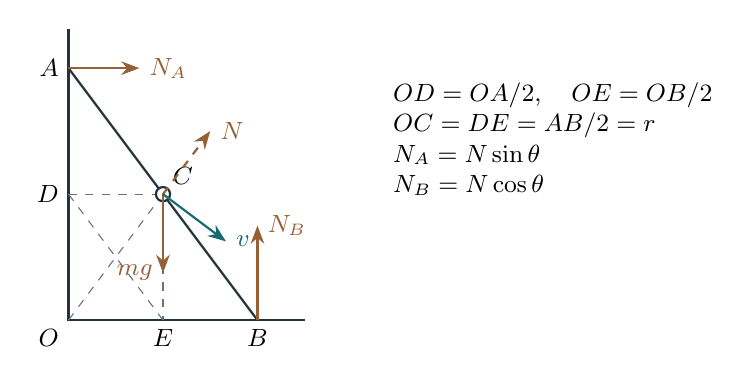
\begin{tikzpicture}
\coordinate(O)at(0,0);\coordinate(A)at(0,3.2);\coordinate(B)at(2.4,0);
\coordinate(C)at(1.2,1.6);\coordinate(D)at(0,1.6);\coordinate(E)at(1.2,0);
\draw[object] (0,3.7)--(O)--(3,0);\draw[object] (A)--(B);
\draw[guide] (D)--(C)--(E);\draw[guide] (D)--(E);\draw[guide] (O)--(C);
\filldraw[object,fill=white] (C) circle(.09);
\foreach \p/\pos in {O/below left,A/left,B/below,C/above right,D/left,E/below}{\node[\pos] at (\p) {$\p$};}
\draw[force] (A)--(.9,3.2) node[right] {$N_A$};
\draw[force] (B)--(2.4,1.2) node[right] {$N_B$};
\draw[force] (C)--(1.2,.6) node[left] {$mg$};
\draw[force,dashed] (C)--(1.8,2.4) node[right] {$N$};
\draw[motion] (C)--(2,1) node[right] {$v$};
\node[align=left,anchor=west] at (4,2.3) {$OD=OA/2,\quad OE=OB/2$\\
$OC=DE=AB/2=r$\\
$N_A=N\sin\theta$\\$N_B=N\cos\theta$};
\end{tikzpicture}
\figcaption{解图3.7B\quad 中点几何决定$C$的轨迹；两支持力的合力可等效移至$C$，并沿$OC$向外。}
\end{minipage}\end{center}

两个支持力的合力方向还可从力矩和分量直接求出。$C$上方的$A$到$C$竖直距离为$r\cos\theta$，
右侧的$B$到$C$水平距离为$r\sin\theta$。
两力的力矩相反，零转动惯量模型要求
$N_A r\cos\theta-N_B r\sin\theta=0$。
因此只要两端仍接触，便有
\[
N_A=N\sin\theta=mg(3\cos\theta-2)\sin\theta,
\quad N_B=N\cos\theta=mg(3\cos\theta-2)\cos\theta.
\]
$0<\theta<\theta_d$内两者非负，在$\theta_d$同时降至零。
若继续强制中心沿圆弧，随后的$3\cos\theta-2<0$就要求墙、地面拉杆，
这与两处只能提供压力的条件不相容。因此圆弧阶段在两支持力共同降为零时结束。脱离瞬间两端仍在接触位置，此后中心沿当时的切线速度进入抛体运动。

图3.7C 说明离位后两端能同时离开接触面。令 $s=OC$，把抛体坐标代入 $s^2=x^2+y^2$。在离位点有 $x_dv_{dx}+y_dv_{dy}=0$ 和 $v_d^2=gy_d$，因此
\[
s^2-r^2=-g v_{dy}\tau^3+\tfrac14g^2\tau^4>0\qquad(\tau>0).
\]
这里 $v_{dy}<0$。在中心触地以前，$x,y$ 均为正，零惯量轻杆可取 $\sin\theta=x/s,\ \cos\theta=y/s$。此时墙端的水平坐标为 $x(1-r/s)>0$，地面端的高度为 $y(1-r/s)>0$，与抛体过程的两个零反力相容。这个取向在离位瞬间接续双接触姿态，因为 $s=r$、$\dot s=0$。有质量的杆还要满足转动方程，其后续姿态和接触力需另求。

\begin{center}\begin{minipage}{.97\linewidth}\centering
\begin{tikzpicture}[scale=.94,transform shape]
\coordinate (O) at (0,0);
\coordinate (C) at (2.07,1.19);
\pgfmathsetmacro{\sC}{sqrt(2.07^2+1.19^2)}
\coordinate (A) at ({2.07*(1-1.56/\sC)},{1.19*(1+1.56/\sC)});
\coordinate (B) at ({2.07*(1+1.56/\sC)},{1.19*(1-1.56/\sC)});
\draw[object](0,2.6)--(O)--(4.45,0);
\draw[guide](0,1.56) arc(90:0:1.56);
\draw[guide](O)--(C) node[pos=.4,below right]{$s$};
\draw[object](A)--(B);
\fill(A)circle(1.6pt)node[above]{$A$};
\fill[accent](C)circle(1.7pt)node[above right]{$C$};
\fill(B)circle(1.6pt)node[above right]{$B$};
\node[below left]at(O){$O$};
\draw[<->] (A)--(0,{1.19*(1+1.56/\sC)});
\draw[<->] (B)--({2.07*(1+1.56/\sC)},0);
\node[align=left,right]at(4.1,1.6){墙端间隙 $x(1-r/s)$\\地面端间隙 $y(1-r/s)$};
\end{tikzpicture}
\figcaption{解图3.7C\quad 离位阶段 $s>r$。图中将两端与墙、地面的间隙放大。}
\end{minipage}\end{center}

\subsubsection*{把落地根式逐步整理}
代入离位竖直速度，有
\[
\begin{aligned}
\tau_{\rm land}
&=\frac{-\sqrt{10gr/27}+\sqrt{46gr/27}}g\\
&=\sqrt{\frac r{27g}}(\sqrt{46}-\sqrt{10})>0.
\end{aligned}
\]
另一根的分子是两个负数之和，对应把抛物线倒推到离位前的数学交点，应舍去。
水平位移中的根式乘法为
\[
\begin{aligned}
v_{dx}\tau_{\rm land}
&=\sqrt{\frac{8gr}{27}}\sqrt{\frac r{27g}}
(\sqrt{46}-\sqrt{10})\\
&=\frac r{27}(\sqrt{368}-\sqrt{80})
=\frac{4r}{27}(\sqrt{23}-\sqrt5).
\end{aligned}
\]
再加上已经走过的$x_d=\sqrt5r/3=9\sqrt5r/27$，
才得到$[5\sqrt5+4\sqrt{23}]r/27$。
最终落点大于离位点的横坐标，却不等于仅有抛体段的水平射程。
全过程中心下降$r$，故碰地前速率平方应为$2gr$；
抛体计算所得$v_x^2=8gr/27$、$v_y^2=46gr/27$的和也为$2gr$，
这与中心从高度 $r$ 降到地面所减少的势能 $mgr$ 一致。


\Needspace{18\baselineskip}

\pdfbookmark[2]{第 8 题 轻杆小球跌落与触地速度}{q8}

\section*{第 8 题\quad 轻杆小球跌落与触地速度}

\tagline{M-03-08}

长 $L$ 的理想轻杆，上端固定一质量为 $m$ 的小球，下端支在粗糙水平地面。由近似竖直位置静止释放，球向右下落。设下端在失去地面支持前不滑动（静摩擦系数足够大），杆的质量可忽略。求球第一次碰地前速度的水平、竖直分量；竖直向上取正。

\begin{center}\begin{minipage}{\linewidth}\centering\begin{tikzpicture}
\draw[object](-.7,0)--(3,0);\draw[object](0,0)--(0,2.7);\filldraw[object,fill=white](0,2.7)circle(.14);\node[left]at(0,1.4){$L$};\node[below]at(0,0){$O$};\draw[motion](.3,2.5)--(1,2.3);\node[right]at(.2,2.7){$m$};
\end{tikzpicture}
\figcaption{图 3.8\quad 初始直立状态取无限小扰动的极限。}
\end{minipage}\end{center}

\Needspace{5\baselineskip}\subsection*{解答}

球在支点固定的阶段沿半径$L$的圆弧下落。解图 3.8A 中，失去支持后水平速度保持不变，竖直速度由重力继续改变。
\begin{center}\begin{minipage}{\linewidth}\centering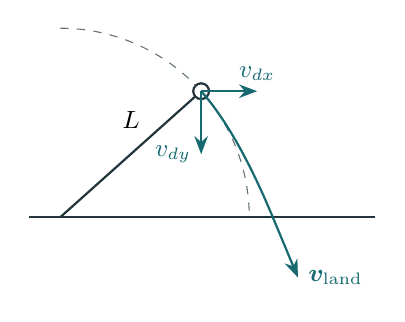
\begin{tikzpicture}
\draw[object](-.4,0)--(4,0);\draw[guide](0,2.4)arc(90:0:2.4);\draw[object](0,0)--(1.789,1.6);\filldraw[object,fill=white](1.789,1.6)circle(.1);\draw[motion](1.789,1.6)--(2.5,1.6)node[above]{$v_{dx}$};\draw[motion](1.789,1.6)--(1.789,.8)node[left]{$v_{dy}$};\draw[traj,domain=0:1,samples=60]plot({1.789+.910*\x},{1.6-1.018*\x-.582*\x^2});
\draw[motion] (2.699,0)--(3.019,-.7673) node[right] {$\vect v_{\mathrm{land}}$};\node[above]at(.9,1){$L$};
\end{tikzpicture}
\figcaption{解图 3.8A\quad 离位时 $\cos\theta_d=2/3$，速度沿切线。}
\end{minipage}\end{center}

\subsubsection*{支点不滑时的圆弧运动}
令杆与竖直方向的夹角为 $\theta$，球位置为 $(L\sin\theta,L\cos\theta)$。支点固定时，杆力沿杆，与球的切线速度垂直，因此不做功。球从高度 $L$ 下降，
\[
v^2=2gL(1-\cos\theta).
\]
设杆对球的作用力 $N$ 沿杆向外为正。径向方程给出
\[
N-mg\cos\theta=-\frac{mv^2}{L},
\qquad N=mg(3\cos\theta-2).
\]
当 $N$ 降为零，地面支持力也降为零。继续沿原圆弧下落会要求地面向下拉杆，故固定支点阶段在这一刻结束，
\[
\cos\theta_d=\frac23,\quad
\sin\theta_d=\frac{\sqrt5}{3},\quad
v_d=\sqrt{\frac{2gL}{3}}.
\]

\subsubsection*{切线分量与自由飞行}
解图 3.8A 中速度指向右下，故
\[
v_{dx}=v_d\cos\theta_d
=\sqrt{\frac{8gL}{27}},\qquad
v_{dy}=-v_d\sin\theta_d
=-\sqrt{\frac{10gL}{27}}.
\]
离位后球仅受重力，水平分量不再变化；竖直方向继续下降 $y_d=2L/3$，所以
\[
v_y^2=v_{dy}^2+2gy_d
=\frac{10gL}{27}+\frac{4gL}{3}
=\frac{46gL}{27}.
\]
碰地前方向向下，应取负根。结果为
\[
\boxed{v_x=\sqrt{\frac8{27}gL},\qquad
v_y=-\sqrt{\frac{46}{27}gL}}.
\]
两分量平方相加得 $v_x^2+v_y^2=2gL$。全过程下降高度 $L$，重力势能减少 $mgL$，正好转为这些动能。

\subsubsection*{不滑动条件}
接触阶段地面所承受的杆力水平、竖直分量分别为 $N\sin\theta,N\cos\theta$，所需静摩擦与支持力之比为 $\tan\theta$。它在这一阶段单调增大，最大值为
\[
\tan\theta_d=\frac{\sqrt5}{2}.
\]
因此题设不滑动可由 $\mu_s\geq\sqrt5/2$ 保证。接触失效时两力同时趋零，以上比值指其左极限。若摩擦不足，支点先滑动，球的圆弧轨迹、离位角和水平速度都需重新求解。
\subsubsection*{把球与支点的受力分别画出}
解图3.8B规定杆力$N$沿杆向外为正。
杆对球的作用力沿右上方；球对杆的反作用力则沿左下方。
无质量杆在接触阶段没有有限的合力与合力矩，
因此地面对杆的向右静摩擦$f_s$与向上支持力$R$分别为
\[
f_s=N\sin\theta,
\qquad R=N\cos\theta.
\]
图3.8B 中，球对杆的水平作用向左，地面对杆的静摩擦因而向右，与该水平分量相抵。
对小球，杆力与切线速度垂直；对杆，地面接触点暂时不动，
所以这两种约束力都不引入额外机械能损失。
\begin{center}\begin{minipage}{\linewidth}\centering
\begin{tikzpicture}
\draw[guide] (0,0)--(1.2,1.2);\filldraw[object,fill=white] (1.2,1.2) circle(.09);
\draw[force] (1.2,1.2)--(1.85,1.85) node[right] {$N$};
\draw[force] (1.2,1.2)--(1.2,-.1) node[right] {$mg$};
\draw[motion] (1.2,1.2)--(1.8,.6) node[right] {$v$};
\node[below] at (.9,-.5) {小球受力};
\draw[object] (4.4,0)--(7,0);\draw[object] (5,0)--(6.2,1.2);
\draw[force] (6.2,1.2)--(5.55,.55) node[above left] {$-N$};
\draw[force] (5,0)--(5,.9) node[left] {$R$};
\draw[force] (5,0)--(5.9,0) node[below] {$f_s$};
\node[below] at (5,-.17) {$O$};\node[below] at (5.7,-.5) {轻杆与地面接触};
\end{tikzpicture}
\figcaption{解图3.8B\quad 作用力与反作用力属于不同物体；支点静摩擦维持的是接触阶段的不滑动。}
\end{minipage}\end{center}

当$N$降到零，$R$与$f_s$同时趋零；继续保持固定支点将需要负的地面支持，因而不再可行。
按理想集中质量轻杆模型，随后小球不受有限的杆力，进入抛体运动。
下端从此随杆移动，$O$ 保留为原支点。理想轻杆采用集中质量极限；若给杆有限质量，杆的转动惯量、动能和接触反力都随之加入运动方程。

\subsubsection*{全程动能与自由飞行中的速度变化}
从初始高度$L$到首次触地，小球的重力势能降低$mgL$，所以
\[
mgL=\frac12m(v_x^2+v_y^2),\qquad v^2=2gL.
\]
离位后没有水平力，故$v_x^2=8gL/27$保持不变；
用全程能量扣除水平动能，直接得到
\[
|v_y|=\sqrt{2gL-\frac{8gL}{27}}
=\sqrt{\frac{46gL}{27}}.
\]
落地时竖直分量向下，按题设正向取$v_y<0$。
全程能量给碰地前的总速率。水平方向的速度由离位前的圆弧速率和切线投影求出；保留这一分量后，剩余的动能才给竖直速度大小。

从离位时的高度和竖直初速度，也可求自由飞行时间：
\[
\tau=\frac{v_{dy}+\sqrt{v_{dy}^2+2g(2L/3)}}g
=\sqrt{\frac L{27g}}(\sqrt{46}-\sqrt{10}).
\]
代入$v_y=v_{dy}-g\tau$，$\sqrt{10gL/27}$两项抵消，
仍得到负的$\sqrt{46gL/27}$。解图3.8A中起点箭头为离位速度分量，
落点的斜箭头为碰地前速度；水平分量相同，竖直分量的绝对值已经增加。


\Needspace{18\baselineskip}

\pdfbookmark[2]{第 9 题 绳绕钉运动与碰钉条件}{q9}

\section*{第 9 题\quad 绳绕钉运动与碰钉条件}

\tagline{M-03-09}

长 $2l$ 的理想细绳，一端固定在钉子 $A$，另一端系小球。小球初始位于 $A$ 右侧同一水平线上，以竖直向下初速度 $v_0$ 运动。钉子 $B$ 位于 $A$ 左侧，$AB=l$。绳转到 $B$ 后，小球绕 $B$ 上行。求小球直接碰到 $A$ 所需的最小初速，允许松绳后以抛体轨迹命中。

\begin{center}\begin{minipage}{\linewidth}\centering\begin{tikzpicture}
\fill(0,0)circle(2pt);\fill(-1.5,0)circle(2pt);\draw[object](0,0)--(3,0);\filldraw[object,fill=white](3,0)circle(.1);\node[above]at(0,0){$A$};\node[above]at(-1.5,0){$B$};\draw[motion](3,0)--(3,-1)node[right]{$v_0$};\draw[guide](3,0)arc(0:-180:3);\draw[<->](-1.5,.65)--(0,.65)node[midway,above]{$l$};
\end{tikzpicture}
\figcaption{图 3.9\quad 先绕 $A$ 经过下半圆，再绕 $B$ 向上运动。}
\end{minipage}\end{center}

\Needspace{5\baselineskip}\subsection*{解答}

小球到 $A$ 左侧 $2l$ 处时速度仍为 $v_0$。改绕 $B$ 后，令松绳点 $D=(-l\cos\theta,l\sin\theta)$（以 $B$ 为原点），如解图 3.9A。
\begin{center}\begin{minipage}{\linewidth}\centering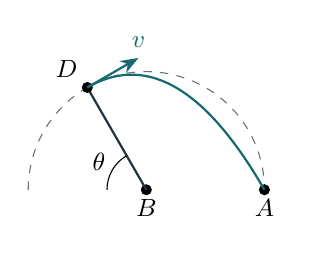
\begin{tikzpicture}
\draw[guide](-1.5,0)arc(180:0:1.5);\fill(0,0)circle(2pt);\fill(1.5,0)circle(2pt);\node[below]at(0,0){$B$};\node[below]at(1.5,0){$A$};\coordinate(D)at(-.75,1.299);\draw[object](0,0)--(D);\fill(D)circle(2pt);\node[above left]at(D){$D$};\draw[motion](D)--(-.1,1.674)node[above]{$v$};\draw[traj,domain=0:2.25,samples=40]plot({-.75+\x},{1.299+.57735*\x-.5132*\x^2});\draw(-.5,0)arc(180:120:.5);\node at(-.6,.35){$\theta$};
\end{tikzpicture}
\figcaption{解图 3.9A\quad 最小初速对应 $\theta=60^\circ$ 时松绳，随后命中 $A$。}
\end{minipage}\end{center}

\subsubsection*{绕钉前后的能量}
小球先绕 $A$ 走下半圆，到达 $A$ 左侧同高位置时，速率又为 $v_0$；这一阶段绳张力为正。绳接触 $B$ 后，有效半径变为 $l$。
以 $B$ 为原点，令球在上行段的位置为
\[
(x,y)=(-l\cos\theta,l\sin\theta),\quad 0<\theta<\pi.
\]
在从左端上升到松绳点的阶段，
\[
v^2=v_0^2-2gl\sin\theta.
\]
指向 $B$ 的重力分量为 $mg\sin\theta$，径向方程是
\[
T+mg\sin\theta=\frac{mv^2}{l}.
\]
因此 $T=0$ 时有 $v^2=gl\sin\theta$，与能量式联立：
\[
v_0^2=3gl\sin\theta.
\]

\subsubsection*{抛体经过目标的条件}
若在上升到最高点之前松绳，$0<\theta<\pi/2$，其切线速度为 $(v\sin\theta,v\cos\theta)$。如解图 3.9A，目标 $A=(l,0)$，故
\[
l=-l\cos\theta+v\sin\theta\,\tau,
\]
\[
0=l\sin\theta+v\cos\theta\,\tau-\frac12g\tau^2.
\]
第一式给出 $\tau=l(1+\cos\theta)/(v\sin\theta)>0$。代入第二式，再代入 $v^2=gl\sin\theta$，约去非零因子后得到
\[
1-3\cos^2\theta-2\cos^3\theta=0.
\]
等价地，
\[
(2\cos\theta-1)(\cos\theta+1)^2=0.
\]
符合上行松绳范围的根只有 $\cos\theta=1/2$，即 $\theta=60^\circ$。于是
\[
\boxed{v_{0,\min}=\sqrt{\frac{3\sqrt3}{2}\,gl}}.
\]

\subsubsection*{两条命中路径与绳长条件}
若全程张紧经过绕 $B$ 的上半圆，最高点要求 $v_{\mathrm{top}}^2\geq gl$，所以 $v_0^2\geq3gl$，所需初速更大。小于抛体命中值的初速又不能满足上述唯一的命中根，因此所得初速是最小值。

松绳后，球到 $B$ 的距离至多为 $l$，因此还要沿这段抛体轨道计算到 $B$ 的距离。令 $z=v\tau/l$，在 $\theta=60^\circ$ 的轨道上，
\[
\frac{x}{l}=-\frac12+\frac{\sqrt3}{2}z,\qquad
\frac{y}{l}=\frac{\sqrt3}{2}+\frac12z-\frac{z^2}{\sqrt3}.
\]
从松绳到命中，$0\leq z\leq\sqrt3$，直接计算
\[
\frac{x^2+y^2}{l^2}-1=\frac{z^3(z-\sqrt3)}3\leq0.
\]
球始终位于以 $B$ 为圆心、半径 $l$ 的圆内，直到目标处才再次达到绳长。因此这段抛体轨道与松绳约束相容。
\subsubsection*{绕钉前后的张力及首次松绳位置}
先写绕$A$下半圆时的速率和张力。以初始水平线为势能零点，
令该段位置角$\gamma$从右端沿顺时针量起，$0\leq\gamma\leq\pi$。
球的高度为$-2l\sin\gamma$，能量与径向方程分别给出
\[
v_A^2=v_0^2+4gl\sin\gamma,
\qquad T_A-mg\sin\gamma=\frac{mv_A^2}{2l},
\]
所以$T_A=mv_0^2/(2l)+3mg\sin\gamma>0$。
该段不会先松绳，到左端时$\sin\gamma=0$，速率确实回到$v_0$，方向竖直向上。
绳的中点在这一刻碰到$B$，速度与新半径仍然垂直，因此不需要切向冲量，也没有动能突失。

绕$B$上行后，张力随位置变化的完整函数是
\[
T_B=\frac m l(v_0^2-2gl\sin\theta)-mg\sin\theta
=\frac{mv_0^2}{l}-3mg\sin\theta.
\]
若$0<v_0^2<3gl$，从$\theta=0$开始张力为正，随上升不断减小，
第一次到零满足$\sin\theta=v_0^2/(3gl)$。
同一圆周公式的速度零点由能量式给出，应有$\sin\theta=v_0^2/(2gl)$，
其值更大，所以球先到张力零点，再转入自由飞行。图B 的圆周公式在张力零点后改用虚线表示延长的数值。
解图3.9B将速度平方与张力同时画出，松绳处的速率仍不为零。
\begin{center}\begin{minipage}{\linewidth}\centering
\begin{tikzpicture}[x=4cm,y=1.05cm]
\draw[axis] (-.05,0)--(1.22,0) node[right] {$u=\sin\theta$};
\draw[axis] (0,-.5)--(0,2.95) node[above] {归一化量};
\draw[traj,domain=0:.866025] plot(\x,{2.598076-2*\x});
\draw[force,domain=0:.866025] plot(\x,{2.598076-3*\x});
\draw[traj,dashed,domain=.866025:1] plot(\x,{2.598076-2*\x});
\draw[force,dashed,domain=.866025:1] plot(\x,{2.598076-3*\x});
\draw[guide] (.866025,0)--(.866025,.866025);
\fill (.866025,0) circle(1.7pt);\fill (.866025,.866025) circle(1.7pt);
\node[above] at (.5,1.598076) {$v^2/(gl)$};
\node[below left] at (.5,1.098076) {$T_B/(mg)$};
\node[below] at (.866025,-.05) {$\sqrt3/2$};
\node[align=left] at (1.8,1.8) {$v_0^2/(gl)=3\sqrt3/2$\\
实线：张紧阶段\\虚线：同一圆周公式的延拓\\松绳时$v^2/(gl)=\sqrt3/2$};
\end{tikzpicture}
\figcaption{解图3.9B\quad 张力为零时转入抛体，实线给出张紧阶段，虚线是圆周公式的延长值。}
\end{minipage}\end{center}

\subsubsection*{以松绳点为原点的目标位移与命中方程}
也可把坐标原点移至松绳点$D$。此时目标位移为
\[
X_A=l(1+\cos\theta),\qquad Y_A=-l\sin\theta.
\]
发射速度与水平正向的夹角为$\alpha=\pi/2-\theta$，
故$\tan\alpha=\cot\theta$、$v\cos\alpha=v\sin\theta$。
从参数式消去时间，得到
\[
Y=X\cot\theta-\frac{gX^2}{2v^2\sin^2\theta}.
\]
将目标坐标和$v^2=gl\sin\theta$全部代入，逐项除以$l$，有
\[
-\sin\theta=\frac{(1+\cos\theta)\cos\theta}{\sin\theta}
-\frac{(1+\cos\theta)^2}{2\sin^3\theta}.
\]
以 $D$ 为原点时，目标在 $D$ 下方，$Y_A=-l\sin\theta$。以 $B$ 为原点时目标高度为零，两者相差的量就是 $D$ 的高度。
令$c=\cos\theta$，乘以$2\sin^3\theta$后整理：
\[
2(1-c^2)^2+2c(1+c)(1-c^2)-(1+c)^2
=1-3c^2-2c^3=0.
\]
等价多项式为$2c^3+3c^2-1$，
把 $(2c-1)(c+1)^2$ 乘开，三次、二次和常数项分别为 $2c^3,3c^2,-1$。
上行段在最高点前松绳，对应 $0<c<1$。其中唯一的根是 $c=1/2$，另一个代数根 $c=-1$ 位于该区间之外，且使消元所除的 $\sin\theta$ 为零。
有效根$c=1/2$使飞行时间为正，与前面以$B$为原点的计算相同。

最后比较两条直接命中路径。全程张紧时，
$T_B$在上半圆最高点最小，要求$v_0^2\geq3gl$；
先松绳再直接命中只需$v_0^2=(3\sqrt3/2)gl$，
二者的初动能比为$\sqrt3/2<1$。
在低于完整半圆阈值的首次上行过程中，松绳点由初速唯一确定，
命中方程又只允许$60^\circ$这一有效角度，故更小的初速不能沿这段自由飞行直接命中$A$。
距离不等式给出整段自由飞行都在可用绳长内，所以这条命中路径实际可达。
在最小初速轨道上，飞行参数还可具体写成
$v=v_0/\sqrt3$、$\tau=\sqrt3l/v=3l/v_0$。
抛体最高点由竖直速度降为零确定，其坐标为
$(-l/8,9\sqrt3l/16)$，最大高度仍小于绕$B$圆周的最高点$l$。
小球保留向右的水平速度，因此不必先升到圆周顶部也能越到目标$A$。
这条轨道保留向右的水平运动，所需初动能较小。图中$D$位于$B$的左上方，对应从左端上行过程中张力第一次降为零的位置。



\Needspace{18\baselineskip}

\pdfbookmark[2]{第 10 题 引力追及中的最大间距}{q10}

\section*{第 10 题\quad 引力追及中的最大间距}

\tagline{M-03-10}

惯性系 $S$ 中，质量分别为 $m_1,m_2$ 的质点 $A,B$ 以万有引力相互吸引。起初 $A$ 静止，间距 $l_0$；$B$ 沿连线远离 $A$，速度 $v_0<\sqrt{2Gm_2/l_0}$。外力 $F$ 始终作用于 $B$，使其速度保持 $v_0$。求两点最大间距及达到该间距前外力在 $S$ 中所做的功。

\begin{center}\begin{minipage}{\linewidth}\centering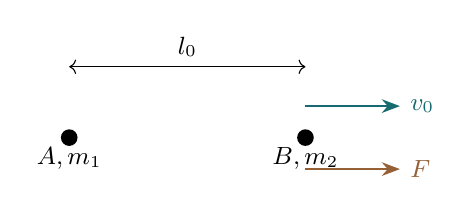
\begin{tikzpicture}
\fill(0,0)circle(3pt);\fill(3,0)circle(3pt);\node[below]at(0,0){$A,m_1$};\node[below]at(3,0){$B,m_2$};\draw[motion](3,.4)--(4.2,.4)node[right]{$v_0$};\draw[force](3,-.4)--(4.2,-.4)node[right]{$F$};\draw[<->](0,.9)--(3,.9)node[midway,above]{$l_0$};
\end{tikzpicture}
\figcaption{图 3.10\quad $F$ 抵消 $B$ 所受引力，$A$ 则不断加速。}
\end{minipage}\end{center}

\Needspace{5\baselineskip}\subsection*{解答}

以匀速运动的 $B$ 为参考系，它仍是惯性系。解图 3.10A 中，$A$ 初速为 $-v_0$；两点最远时 $A$ 的相对速度降到零。
\begin{center}\begin{minipage}{\linewidth}\centering\begin{tikzpicture}
\fill(0,0)circle(3pt);\fill(3,0)circle(3pt);\node[below]at(0,0){$A$};\node[below]at(3,0){$B$（静止）};\draw[motion](0,.4)--(-1.2,.4)node[left]{$-v_0$};\draw[force](0,-.4)--(1.2,-.4)node[right]{引力};\node[align=left]at(5,1){$B$ 系：外力功为零\\$S$ 系：外力功非零};
\end{tikzpicture}
\figcaption{解图 3.10A\quad 能量守恒可在 $B$ 系使用，外力功须回到指定参考系计算。}
\end{minipage}\end{center}

\subsubsection*{最大间距对应相对速度为零}
取 $S$ 系中从 $A$ 指向 $B$ 的方向为正。$B$ 始终以速度 $v_0$ 匀速运动，故可选择随 $B$ 平移的惯性系。在该系中，$B$ 固定，$A$ 的初速为 $-v_0$，先远离 $B$，再在引力下减速。
间距的变化率为 $\dot l=v_0-v_A$。最远时 $\dot l=0$，即 $S$ 系中 $v_A=v_0$；解图 3.10A 对应的 $B$ 系速度则为零。

\subsubsection*{在随动惯性系求距离}
维持 $B$ 匀速的外力作用点在 $B$ 系不移动，因此不做功。两点引力势能为 $-Gm_1m_2/l$，能量守恒为
\[
\frac12m_1v_0^2-\frac{Gm_1m_2}{l_0}
=-\frac{Gm_1m_2}{l_{\max}}.
\]
约去 $m_1$ 后，
\[
\frac1{l_{\max}}=\frac1{l_0}-\frac{v_0^2}{2Gm_2},
\]
\[
\boxed{l_{\max}=\frac{2Gm_2l_0}{2Gm_2-l_0v_0^2}}.
\]
题设的速度上限保证分母为正。它不含 $m_1$，因为在给定 $B$ 运动的条件下，$A$ 的引力加速度与自身质量无关。

\subsubsection*{回到指定参考系求功}
在 $S$ 系中，$B$ 的动能不变，$A$ 的动能从零增至 $m_1v_0^2/2$；势能增加量为
\[
\Delta U=Gm_1m_2\left(\frac1{l_0}-\frac1{l_{\max}}\right)
=\frac12m_1v_0^2.
\]
由系统功能关系，
\[
W=\Delta K+\Delta U
=\frac12m_1v_0^2+\frac12m_1v_0^2,
\qquad \boxed{W=m_1v_0^2}.
\]
作用于 $B$ 的外力与作用于 $A$ 的引力大小相等、方向相同。因而外力冲量也等于 $A$ 的动量增量 $m_1v_0$。其作用点速度恒为 $v_0$，所以 $W=v_0\int F\,\dd t=m_1v_0^2$。

$v_0\to0$ 时 $l_{\max}\to l_0$、功趋零；$v_0$ 趋近给定临界值时，最大间距趋于无穷。外力作用点在 $B$ 系的位移为零，在 $S$ 系随 $B$ 向右运动。力与作用点位移的乘积因此在两系分别给零功和正功。
\subsubsection*{先在指定参考系把两端能量写全}
取解图3.10A中从$A$指向$B$的方向为正。
在$S$系，初态与最大间距状态的机械能分别为
\[
E_i=\frac12m_2v_0^2-\frac{Gm_1m_2}{l_0},\qquad
E_f=\frac12(m_1+m_2)v_0^2-\frac{Gm_1m_2}{l_{\max}}.
\]
外力只作用在$B$上，系统功能关系仍须同时计算两个质点的动能与它们的相互作用势能，故
\[
W=E_f-E_i
=\frac12m_1v_0^2+Gm_1m_2\left(\frac1{l_0}-\frac1{l_{\max}}\right).
\]
$B$ 的动能在两端相同，而 $A$ 的动能和引力势能分别增加。它们的改变量组成这个 $W$。
换到$B$系后，初始只有$A$有动能，最远处二者瞬时均静止；
外力作用点固定，所以才可以用零外力功把这一距离求出，再回到$S$系代入。

\subsubsection*{用相对运动方程证明最大间距唯一}
维持$B$匀速所需的力为$F=Gm_1m_2/l^2$，始终向右。
$A$在$S$系满足$\dot v_A=Gm_2/l^2$，因此
\[
\dot l=v_0-v_A,\qquad
\ddot l=-\frac{Gm_2}{l^2}<0.
\]
间距的变化率严格减小，初始为$v_0>0$，故若有有限零点，它只可能是唯一的最大值点。
将相对方程乘以$\dot l$，积分并代入$l=l_0,\dot l=v_0$，得到
\[
\frac12\dot l^{\,2}-\frac{Gm_2}{l}
=\frac12v_0^2-\frac{Gm_2}{l_0},
\qquad
\dot l^{\,2}=2Gm_2\left(\frac1l-\frac1{l_{\max}}\right).
\]
在向外分离阶段应取$\dot l>0$的根。
题设相对能量为负，故存在有限$l_{\max}>l_0$；
若$v_0^2=2Gm_2/l_0$，零点只能在无穷远达到；再增大初速，间距将一直增长。
解图3.10B显示最大距离时两条位置曲线切线平行，两质点在$S$系仍以同一非零速度前进。
\begin{center}\begin{minipage}{\linewidth}\centering
\begin{tikzpicture}
\draw[axis] (-.2,0)--(4.25,0) node[right] {$x/l_0$};
\draw[axis] (0,-.2)--(0,3.35) node[above] {$v_0t/l_0$};
\draw[traj,domain=0:1,samples=100] plot({1+pi/2*\x-cos(90*\x)-sin(90*\x)},{1+pi/2*\x-cos(90*\x)});
\draw[object] (1,0)--(3.570796,2.570796);
\draw[guide] (0,2.570796)--(3.570796,2.570796);
\fill (1.570796,2.570796) circle(1.7pt);\fill (3.570796,2.570796) circle(1.7pt);
\draw[motion] (1.17,2.17)--(1.97,2.97);
\draw[motion] (3.17,2.17)--(3.97,2.97);
\draw[<->] (1.570796,3.1)--(3.570796,3.1) node[midway,above] {$l_{\max}/l_0=2$};
\node[above left] at (.1,1.1) {$A$};\node[right] at (2.3,1.2) {$B$};
\node[below] at (1,0) {$1$};
\node[align=left,anchor=west] at (4.8,1.6) {示例：$v_0^2=Gm_2/l_0$\\
$B$的位置—时间线为直线\\$A$从静止加速\\最远时两切线平行\\两者在 $S$ 系以同速前进};
\end{tikzpicture}
\figcaption{解图3.10B\quad 位置—时间图中的间距；图中最大距离是同一时刻两点横坐标之差。}
\end{minipage}\end{center}

从相对速度对间距积分，可以求出到达最远处的时刻。
令$\kappa=Gm_2$、$q=l_0/l_{\max}\in(0,1)$，则
\[
t_{\max}=\int_{l_0}^{l_{\max}}
\frac{\dd l}{\sqrt{2\kappa(1/l-1/l_{\max})}}.
\]
作$l=l_{\max}\sin^2\psi$的代换，积分化为
$2\sqrt{l_{\max}^3/(2\kappa)}\int\sin^2\psi\,\dd\psi$，
上下限为$\arcsin\sqrt q$和$\pi/2$，所以
\[
t_{\max}=\sqrt{\frac{l_{\max}^3}{2\kappa}}
\left(\arccos\sqrt q+\sqrt{q(1-q)}\right).
\]
有限距离处虽有$\dot l=0$，积分端点只呈反平方根奇性，所需时间仍有限。

最后，恒速参考系变换中的功也可直接对应。
系统总动量为$P$，伽利略变换给
$E'=E-v_0P+\frac12(m_1+m_2)v_0^2$。
初、终态质量不变，故
\[
\Delta E'=\Delta E-v_0\Delta P,
\qquad 0=W-v_0(m_1v_0).
\]
$B$的动量前后相同，增加的总动量全是$A$的$m_1v_0$。
两参考系的能量改变量不同，恰好相差平移速度乘外力冲量，与所求外力功一致。


\Needspace{18\baselineskip}

\pdfbookmark[2]{第 11 题 地球直通隧道中的运动}{q11}

\section*{第 11 题\quad 地球直通隧道中的运动}

\tagline{M-03-11}

将地球看作半径 $R$、密度均匀且不自转的球体，地表重力加速度为 $g$。在地表两点 $A,B$ 间开一直通光滑隧道，长度为 $L$。小球从 $A$ 静止释放，忽略空气及其他阻力。求最大速率和首次从 $A$ 到 $B$ 的时间。

\begin{center}\begin{minipage}{\linewidth}\centering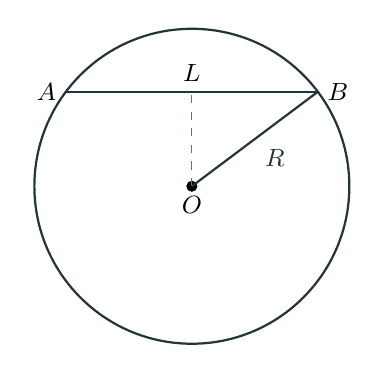
\begin{tikzpicture}
\draw[object](0,0)circle(2);\draw[object](-1.6,1.2)--(1.6,1.2);\fill(0,0)circle(2pt);\node[below]at(0,0){$O$};\node[left]at(-1.6,1.2){$A$};\node[right]at(1.6,1.2){$B$};\draw[guide](0,0)--(0,1.2);\draw[object](0,0)--(1.6,1.2)node[midway,below right]{$R$};\node[above]at(0,1.2){$L$};
\end{tikzpicture}
\figcaption{图 3.11\quad 隧道方向的引力分量指向隧道中点。}
\end{minipage}\end{center}

\Needspace{5\baselineskip}\subsection*{解答}

均匀球内部的引力为 $\vect F=-(mg/R)\vect r$。以隧道中点 $C$ 为原点，沿隧道取坐标 $s$，解图 3.11A 表明只有沿隧道的分量参与运动。
\begin{center}\begin{minipage}{\linewidth}\centering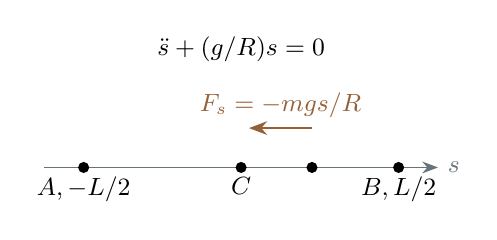
\begin{tikzpicture}
\draw[axis](-2.5,0)--(2.5,0)node[right]{$s$};\fill(-2,0)circle(2pt);\fill(0,0)circle(2pt);\fill(2,0)circle(2pt);\node[below]at(-2,0){$A,-L/2$};\node[below]at(0,0){$C$};\node[below]at(2,0){$B,L/2$};\fill(.9,0)circle(2pt);\draw[force](.9,.5)--(.1,.5)node[midway,above]{$F_s=-mgs/R$};\node at(0,1.5){$\ddot s+(g/R)s=0$};
\end{tikzpicture}
\figcaption{解图 3.11A\quad 幅度为 $L/2$ 的简谐运动，$A$ 到 $B$ 恰为半周期。}
\end{minipage}\end{center}

\subsubsection*{薄球壳对内部点的引力相消}
先证明球壳结论。取面密度为 $\sigma$ 的均匀薄球壳和壳内一点 $P$。如解图 3.11B，从 $P$ 发出一对方向相反、立体角同为 $\dd\Omega$ 的微小锥束，与球面截出面元 $\dd S_1,\dd S_2$。记距离为 $s_1,s_2$，面元外法线与相应视线的锐夹角为 $\beta_1,\beta_2$。
\begin{center}\begin{minipage}{\linewidth}\centering\begin{tikzpicture}
\draw[object] (0,0) circle(2);
\coordinate (P) at (.65,.45);
\fill[accent!13] (P)--(1.9132121,0.5827689)--(1.9757252,0.3106607)--cycle;
\fill[accent!13] (P)--(-1.8679608,0.7146483)--(-1.9925683,0.1722549)--cycle;
\draw[guide] (1.9132121,0.5827689)--(-1.9925683,0.1722549);
\draw[guide] (1.9757252,0.3106607)--(-1.8679608,0.7146483);
\coordinate (S1) at (1.9487175,0.4500000);
\coordinate (S2) at (-1.9487175,0.4500000);
\draw[object] (S2)--(S1);\draw[guide] (0,0)--(S1);\draw[guide] (0,0)--(S2);
\draw[force] (P)--(1.4,.45) node[midway,above] {$\mathrm dF_1$};
\draw[force] (P)--(-.1,.45) node[midway,above] {$\mathrm dF_2$};
\fill (P) circle(2pt) node[below] {$P$};\fill (0,0) circle(1.5pt) node[below] {$O$};
\draw[force] (S1)--(2.5333328,0.5850000) node[right] {$\vect n_1$};
\draw[force] (S2)--(-2.5333328,0.5850000) node[left] {$\vect n_2$};
\draw[very thick,accent] (1.9757252,0.3106607) arc(8.9359551:16.9408603:2);
\draw[very thick,accent] (-1.8679608,0.7146483) arc(159.0640449:175.0591397:2);
\node[above right] at (1.8,1) {$\mathrm dS_1$};\node[above left] at (-1.75,1.2) {$\mathrm dS_2$};
\draw[<->] (.65,-.25)--(1.948717,-.25) node[midway,below] {$s_1$};
\draw[<->] (-1.948717,-.85)--(.65,-.85) node[midway,below] {$s_2$};
\node at (0,2.55) {两锥束的边缘射线均通过 $P$};
\node at (0,-2.5) {$\beta_1=\beta_2$，对应面元的投影与距离平方相消};
\end{tikzpicture}
\figcaption{解图3.11B\quad 反向等立体角锥束截出的两个面元，距离较远的一端截面较大。}
\end{minipage}\end{center}
两面元处在同一条过 $P$ 的弦两端。两条球半径与弦构成等腰三角形，故 $\beta_1=\beta_2=\beta$。面元在视线垂直面上的投影给出
\[
\dd\Omega=\frac{\dd S_1\cos\beta}{s_1^2}
=\frac{\dd S_2\cos\beta}{s_2^2},\qquad
\frac{\dd S_1}{s_1^2}=\frac{\dd S_2}{s_2^2}.
\]
两面元对 $m$ 的引力大小分别为
\[
\dd F_1=\frac{Gm\sigma\dd S_1}{s_1^2},\qquad
\dd F_2=\frac{Gm\sigma\dd S_2}{s_2^2}.
\]
它们大小相等、方向相反。把所有锥束对应的面元配对积分，便得壳内合引力为零。均匀实心球可分解成同心薄壳，因此位于小球半径以外的各壳都不贡献合引力。

\subsubsection*{球内引力为何正比于距离}
设地球总质量为 $M_E$。均匀密度下，半径 $r$ 以内的质量为 $M_Er^3/R^3$；在这一半径以外的球壳对内部点的合引力为零。小球所受引力因而为
\[
F(r)=Gm\frac{M_Er^3/R^3}{r^2}
=\frac{GM_Em}{R^3}r=\frac{mg}{R}r,
\]
方向指向地心，其中使用了地表关系 $g=GM_E/R^2$。球内引力随 $r$ 线性变化，其中的等效质量是半径 $r$ 内包围的 $M_Er^3/R^3$。

\subsubsection*{以无穷远为零点的完整势能}
沿地心径向向外为正，引力分量在球内为 $F_r=-GM_Emr/R^3$，球外为 $F_r=-GM_Em/r^2$。由 $U(\infty)=0$ 和 $F_r=-\dd U/\dd r$，到球内一点的势能由球内、球外两段积分相加，
\[
\begin{aligned}
U(r)&=\int_r^R\left(-\frac{GM_Em}{R^3}\xi\right)\dd\xi
 +\int_R^\infty\left(-\frac{GM_Em}{\xi^2}\right)\dd\xi\\
&=-\frac{GM_Em}{2R^3}(R^2-r^2)-\frac{GM_Em}{R}\\
&=\frac{GM_Em}{2R^3}(r^2-3R^2).
\end{aligned}
\]
在地表 $U(R)=-GM_Em/R$，与外部势能连续。从隧道端点静止释放，到距地心 $r$ 处时，
\[
\frac12mv^2=U(R)-U(r)
=\frac{GM_Em}{2R^3}(R^2-r^2),\qquad
v^2=\frac gR(R^2-r^2).
\]
球外部分的积分确定了常量 $-GM_Em/R$。于是球内和球外势能在地表接上，并共同采用无穷远的零点。

\subsubsection*{投影到任意直隧道}
以隧道中点 $C$ 为原点，$s$ 沿隧道指向 $B$，地心到隧道的垂线向量记为 $\vect d$。任意位置的地心位矢为 $\vect r=\vect d+s\vect e_s$。
引力向量为 $-(mg/R)\vect r$；其中垂直隧道的分量由隧道支持力平衡，沿隧道的分量为
\[
F_s=-\frac{mg}{R}s.
\]
解图3.11A 中，地心在隧道上的垂足是中点 $C$，沿程回复力始终指向 $C$。因此
\[
\ddot s+\omega^2s=0,\qquad \omega=\sqrt{\frac gR}.
\]
初始 $s(0)=-L/2,\dot s(0)=0$，解为
\[
s(t)=-\frac L2\cos\omega t,\qquad
\dot s(t)=\frac{L\omega}{2}\sin\omega t.
\]
到中点时速率最大，到另一端时第一次再静止，故
\[
\boxed{v_{\max}=\frac L2\sqrt{\frac gR}},\qquad
\boxed{t_{AB}=\frac{\pi}{\omega}=\pi\sqrt{\frac Rg}}.
\]

\subsubsection*{沿程势能与通行时间积分}
由解图 3.11A，$r^2=d^2+s^2$、$R^2=d^2+(L/2)^2$，代入完整势能式，固定的 $d^2$ 项在能量差中抵消。略去与位置无关的常量后，有效的一维势能为 $U_s=mgs^2/(2R)$。由两端初态与一般状态的能量关系，
\[
v^2=\frac gR\left[\left(\frac L2\right)^2-s^2\right].
\]
若从 $A$ 起量路程 $x=s+L/2$，则 $v^2=(g/R)x(L-x)$，通行时间为
\[
t_{AB}=\sqrt{\frac Rg}\int_0^L\frac{\dd x}{\sqrt{x(L-x)}}.
\]
令 $x=(L/2)(1-\cos\varphi)$，积分范围变为 $0\leq\varphi\leq\pi$，被积式化为 $\dd\varphi$，仍得到 $\pi\sqrt{R/g}$。
长度 $L$ 改变振幅和最大速率，却不改变半周期；直径隧道和任意弦隧道的通行时间相同，前提是均匀、不自转且无阻力的模型。
\subsubsection*{用端点坐标把几何与积分展开}
记地心到隧道的距离为$d$。题图3.11的直角三角形给出
$d^2=R^2-L^2/4$，故在距$A$为$x$的地方，
\[
r^2=d^2+\left(\frac L2-x\right)^2
=R^2-\frac{L^2}{4}+\frac{L^2}{4}-Lx+x^2
=R^2-Lx+x^2.
\]
代入$v^2=(g/R)(R^2-r^2)$，才得到$v^2=(g/R)x(L-x)$。
$0<x<L$内，
\[
\frac{\dd v}{\dd x}
=\sqrt{\frac gR}\frac{L-2x}{2\sqrt{x(L-x)}}.
\]
它在$x<L/2$为正、$x>L/2$为负，因而中点给出最大速率，
这两个导数符号分别对应前半程加速和后半程减速。

用 $x=L\sin^2\psi$ 作时间积分的代换时，
此时$\dd x=2L\sin\psi\cos\psi\,\dd\psi$，
$\sqrt{x(L-x)}=L\sin\psi\cos\psi$，上下限对应$0$和$\pi/2$，所以
\[
t_{AB}=\sqrt{\frac Rg}\int_0^{\pi/2}2\,\dd\psi
=\pi\sqrt{\frac Rg}.
\]
两端速率虽然为零，被积式只呈$1/\sqrt{x}$或$1/\sqrt{L-x}$型奇性，
积分有限。$
\sqrt{R/g}$具有时间量纲，与$\omega=\sqrt{g/R}$互为倒数，周期中的 $\sqrt{R/g}$ 由这个倒数关系确定。
几何上要求$0<L\leq2R$；短弦极限中振幅、初始沿程加速度和最大速率一起减小，
较短的路程同时对应较小的回复加速度，从静止出发的通行时间保持同一半周期。


\Needspace{18\baselineskip}

\pdfbookmark[2]{第 12 题 旋转杆上双弹簧小球}{q12}

\section*{第 12 题\quad 旋转杆上双弹簧小球}

\tagline{M-03-12}

两个质量均为 $m$ 的小球串在理想光滑轻杆上，杆绕固定点 $O$ 在水平面内转动。两根相同轻弹簧依次连接 $O$、内球、外球，劲度系数均为 $k$，原长均为 $l_0$。角速度由零无限缓慢增加到 $\omega$，径向瞬态振动可忽略。求外力所做的功、两弹簧长度之比，以及这一准静态分支允许的 $\omega$ 范围。

\begin{center}\begin{minipage}{\linewidth}\centering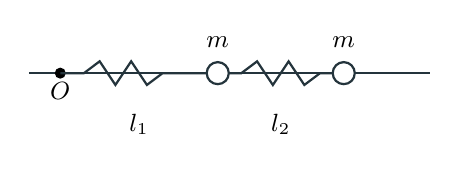
\begin{tikzpicture}
\draw[object](-.4,.2)--(4.7,.2);\fill(0,.2)circle(2pt);\node[below]at(0,.2){$O$};\draw[object](0,.2)--(.3,.2)--(.5,.35)--(.7,.05)--(.9,.35)--(1.1,.05)--(1.3,.2)--(2,.2);\draw[object](2,.2)--(2.3,.2)--(2.5,.35)--(2.7,.05)--(2.9,.35)--(3.1,.05)--(3.3,.2)--(3.6,.2);\filldraw[object,fill=white](2,.2)circle(.14);\filldraw[object,fill=white](3.6,.2)circle(.14);\node[above]at(2,.4){$m$};\node[above]at(3.6,.4){$m$};\node[below]at(1,-.2){$l_1$};\node[below]at(2.8,-.2){$l_2$};
\end{tikzpicture}
\figcaption{图 3.12\quad 外球到转轴的距离为 $l_1+l_2$。}
\end{minipage}\end{center}

\Needspace{5\baselineskip}\subsection*{解答}

令 $q=m\omega^2/k$。解图 3.12A 将两球的径向受力分开；$T_1,T_2$ 分别是内、外弹簧的弹力。
\begin{center}\begin{minipage}{\linewidth}\centering\begin{tikzpicture}
\begin{scope}
\draw[guide](-1.8,0)--(2,0);\filldraw[object,fill=white](0,0)circle(.12);
\draw[force](0,0)--(-1.35,0)node[above,midway]{$T_1$};
\draw[force](0,0)--(1.35,0)node[above,midway]{$T_2$};
\node[below]at(0,-.35){内球 $m$，半径 $l_1$};
\node at(0,-1.1){$T_1-T_2=m\omega^2l_1$};
\end{scope}
\begin{scope}[xshift=5.2cm]
\draw[guide](-1.8,0)--(2,0);\filldraw[object,fill=white](0,0)circle(.12);
\draw[force](0,0)--(-1.35,0)node[above,midway]{$T_2$};
\node[below]at(0,-.35){外球 $m$，半径 $l_1+l_2$};
\node at(0,-1.1){$T_2=m\omega^2(l_1+l_2)$};
\end{scope}
\node at(2.6,1.15){$T_1=k(l_1-l_0),\qquad T_2=k(l_2-l_0)$};
\draw[motion](-2,1.15)--(-3.2,1.15)node[left]{向 $O$};
\end{tikzpicture}
\figcaption{解图 3.12A\quad 分别取内球、外球为对象；力箭头从各自球心出发，向内为径向正向。}
\end{minipage}\end{center}

\subsubsection*{分别列两球的径向方程}
两弹簧长度记为 $l_1,l_2$，内球和外球到轴的距离分别是 $l_1$、$l_1+l_2$。如解图 3.12A，内球受内弹簧向内的力和外弹簧向外的力，外球只受外弹簧向内的力。准静态条件使两球相对杆的径向速度可忽略，故
\[
k(l_1-l_0)-k(l_2-l_0)=m\omega^2l_1,
\]
\[
k(l_2-l_0)=m\omega^2(l_1+l_2).
\]
运动在水平面内，重力由竖直支持力平衡，两条径向方程分别计入沿杆的弹簧力。

令 $q=m\omega^2/k$。第一式给出 $l_2=(1-q)l_1$；代入第二式，
\[
(1-q)l_1-l_0=q(2-q)l_1.
\]
整理得 $D l_1=l_0$，其中 $D=q^2-3q+1$，所以
\[
\boxed{l_1=\frac{l_0}{D},\quad l_2=\frac{(1-q)l_0}{D},
\quad \frac{l_2}{l_1}=1-q}.
\]

\subsubsection*{外力功包括动能与弹性势能}
初态两弹簧都为原长，两球静止，机械能取零。末态实验室系的动能为
\[
K=\frac12m\omega^2\bigl[l_1^2+(l_1+l_2)^2\bigr],
\]
弹性势能为
\[
U=\frac12k(l_1-l_0)^2+\frac12k(l_2-l_0)^2.
\]
径向调速足够缓慢时，两球的径向动能趋于零。转动驱动输入的功积累为实验室系的转动动能与两根弹簧的弹性势能，因而
\[
W=\frac{k}{2}\{q[l_1^2+(l_1+l_2)^2]
+(l_1-l_0)^2+(l_2-l_0)^2\}.
\]
代入长度，完全写成 $\omega$ 的函数为
\[
\boxed{W=\frac{kl_0^2}{2D^2}
\left[q(1+(2-q)^2)+(1-D)^2+(1-q-D)^2\right]}.
\]
若需要多项式形式，展开分子可得
\[
W=\frac{kl_0^2}{2(q^2-3q+1)^2}
\left(2q^4-9q^3+9q^2+5q\right).
\]
小角速度下 $D=1+O(q)$，最低阶 $W=(5/2)kl_0^2q+O(q^2)
=(5/2)m\omega^2l_0^2+O(\omega^4)$，正是近似原长时两球的转动动能。

\subsubsection*{准静态分支的范围}
用 $r_1=l_1,r_2=l_1+l_2$ 表示径向位置，旋转系有效势能为
\[
U_{\mathrm{eff}}=\frac{k}{2}(r_1-l_0)^2
+\frac{k}{2}(r_2-r_1-l_0)^2
-\frac{m\omega^2}{2}(r_1^2+r_2^2).
\]
其二阶矩阵为 $k\begin{pmatrix}2-q&-1\\-1&1-q\end{pmatrix}$。局部极小要求 $2-q>0$ 且行列式 $D>0$。从 $q=0$ 连续增加时，先到达的零点是 $(3-\sqrt5)/2$，故
\[
\boxed{0\leq\omega<
\sqrt{\frac{k}{m}\frac{3-\sqrt5}{2}}}.
\]
在这一范围内两长度均为正。上界处的 $D$ 趋于零，两根平衡长度一起发散。从静止连续增加角速度的准静态过程在这里结束。
\subsubsection*{长度之比、实际伸长与稳定模态}
在允许的分支上$D>0$且$0\leq q<(3-\sqrt5)/2$，
两个弹簧的伸长分别为
\[
l_1-l_0=\frac{q(3-q)}D l_0,
\qquad l_2-l_0=\frac{q(2-q)}D l_0.
\]
$q>0$时两者都为正，内弹簧伸长更多。
因此 $l_2/l_1<1$ 时，两根弹簧都处于拉伸状态，外弹簧的长度和伸长均小于内弹簧。
解图3.12A中$T_1-T_2=m\omega^2l_1>0$也直接给出$T_1>T_2$，
与两伸长之差一致；角速度趋于零时，两伸长都从零连续开始。

对固定角速度下的小径向扰动，二阶矩阵的两个本征值为
\[
\lambda_\pm=\frac k2(3-2q\pm\sqrt5).
\]
由于两球质量相同，扰动方程的两个频率平方为$\lambda_\pm/m$。
最先软化的是负号分支，它在$q=(3-\sqrt5)/2$处降至零。
这与平衡长度分母第一次变零的位置相同，
在同一转速上，径向软模频率归零，平衡长度发散。缓慢调速的物理解支从 $q=0$ 起，到这个首个临界值为止。


\Needspace{18\baselineskip}

\pdfbookmark[2]{第 13 题 旋转圆环中的平衡稳定性}{q13}

\section*{第 13 题\quad 旋转圆环中的平衡稳定性}

\tagline{M-03-13}

半径为 $R$ 的光滑竖直圆环，绕其竖直直径以恒定角速度 $\omega$ 转动。质量为 $m$ 的小球串在环上。用从最低点向右量起的有符号角 $\theta$ 表示位置。求相对圆环的平衡位置并讨论稳定性，包含临界角速度的情形。

\begin{center}\begin{minipage}{\linewidth}\centering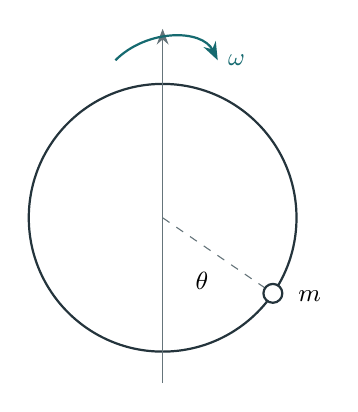
\begin{tikzpicture}
\draw[object](0,0)circle(1.7);\draw[axis](0,-2.1)--(0,2.4);\draw[guide](0,0)--(1.4,-.96);\filldraw[object,fill=white](1.4,-.96)circle(.12);\node[right]at(1.6,-1){$m$};\node at(.5,-.8){$\theta$};\draw[motion](-.6,2)..controls(-.2,2.4)and(.5,2.4)..(.7,2)node[right]{$\omega$};
\end{tikzpicture}
\figcaption{图 3.13\quad 左右对称的非最低点平衡须成对出现。}
\end{minipage}\end{center}

\Needspace{5\baselineskip}\subsection*{解答}

圆环系中，沿环的运动可由有效势能
$U(\theta)=mgR(1-\cos\theta)-m\omega^2R^2\sin^2\theta/2$ 描述。解图 3.13A 示出快转时最低点由势阱变为势垒。
\begin{center}\begin{minipage}{\linewidth}\centering\begin{tikzpicture}
\draw[axis](-2,0)--(2,0)node[right]{$\theta$};\draw[axis](0,-1.2)--(0,1.8)node[above]{$U/(mgR)$};\draw[traj,domain=-1.7:1.7,samples=80]plot(\x,{1-cos(\x r)-.9*sin(\x r)^2});\node[below]at(-.97,-.23){$-\theta_e$};\node[below]at(.97,-.23){$\theta_e$};\node[above left]at(0,0){$0$};\node[align=left]at(4.7,.8){$\omega>\sqrt{g/R}$\\左右出现两个稳定平衡};
\end{tikzpicture}
\figcaption{解图 3.13A\quad 取 $\omega^2R/g=1.8$，有效势能以 $mgR$ 为单位，零点取在环的最低点。}
\end{minipage}\end{center}

\subsubsection*{沿环运动的有效势能}
相对转动圆环，球沿环的速度为 $R\dot\theta$。取环面向右的有符号水平坐标 $\varrho=R\sin\theta$，到转轴的距离为 $|\varrho|$。在随环转动的参考系中，离心力的水平分量为 $m\omega^2\varrho$，随小球处于转轴哪一侧而改变符号。沿环移动 $\dd\theta$ 时，水平位移为 $\dd\varrho=R\cos\theta\dd\theta$。从底点到角度 $\theta$，离心力做功
\[
W_{\rm cf}=\int_0^\theta m\omega^2R^2\sin\xi\cos\xi\,\dd\xi
=\frac12m\omega^2R^2\sin^2\theta.
\]
故取底点为零，离心势能为 $U_{\rm cf}=-W_{\rm cf}$，重力势能为 $U_g=mgR(1-\cos\theta)$。两者相加，
\[
U(\theta)=mgR(1-\cos\theta)
-\frac12m\omega^2R^2\sin^2\theta.
\]
圆环系的沿环运动满足 $mR^2\ddot\theta=-U'(\theta)$，因而 $E_{\rm rot}=mR^2\dot\theta^2/2+U(\theta)$ 为常量。科里奥利力在本题沿环方向没有分量，不进入该一维方程。$E_{\rm rot}$ 是在恒角速度圆环系中得到的守恒量。地面系中，维持圆环匀速转动的装置可以通过环对球做功，因而改变球的机械能。
平衡条件为
\[
U'=mR\sin\theta(g-\omega^2R\cos\theta)=0.
\]
因此底点 $\theta=0$ 和顶点 $\theta=\pi$ 总是平衡；当 $\omega^2R\geq g$ 时，还可能有
\[
\cos\theta_e=\frac{g}{\omega^2R}.
\]
用有符号角表示左右位置，非零平衡须写为 $\theta=\pm\theta_e$。

\subsubsection*{顶点、底点与侧平衡的势能曲率}
二阶导数为
\[
U''=mgR\cos\theta-m\omega^2R^2\cos2\theta.
\]
在顶点，
$U''(\pi)=-mgR-m\omega^2R^2<0$，始终不稳定。
在底点，
\[
U''(0)=mR(g-\omega^2R).
\]
故 $\omega<\sqrt{g/R}$ 时底点稳定，$\omega>\sqrt{g/R}$ 时底点不稳定。
在两个非零平衡处代入 $g=\omega^2R\cos\theta_e$，得到
\[
U''(\pm\theta_e)=m\omega^2R^2\sin^2\theta_e>0,
\]
两处曲率均为正，所以左右侧点都稳定。解图3.13A 中两处势能谷关于 $\theta=0$ 对称，对应这两个位置。

\subsubsection*{临界转速下的四次势阱}
当 $\omega=\sqrt{g/R}$，二阶项恰好相消，底点附近的势能由下一阶决定。展开
\[
1-\cos\theta=\frac{\theta^2}{2}-\frac{\theta^4}{24}+O(\theta^6),
\quad
\sin^2\theta=\theta^2-\frac{\theta^4}{3}+O(\theta^6).
\]
于是
\[
U(\theta)=\frac{mgR}{8}\theta^4+O(\theta^6).
\]
小角度偏离使势能增加，所以底点仍稳定。此时线性恢复项为零，最低阶恢复力矩与 $\theta^3$ 成正比，振动周期随振幅变化。

稳定平衡附近的小振动频率随转速改变。慢转底点的频率为
$\Omega^2=g/R-\omega^2$；快转非零平衡附近为
$\Omega^2=\omega^2\sin^2\theta_e$。无阻尼时，平衡位置附近的微小扰动引起持续的往复运动，振幅由初始位移和速度确定。
\subsubsection*{侧平衡的曲率与临界底点的周期}
平衡位置应按$2\pi$周期理解。慢转时只有底点与顶点两类位置；
当$\omega^2R>g$时，$\cos\theta_e=g/(\omega^2R)$才给出两个不同的侧平衡。
等号时两个侧点并入底点，底部只有一个平衡位置。
将这一余弦逐项代入二阶导数，得到
\[
\begin{aligned}
U''(\theta_e)
&=mR^2\left[\frac gR\frac g{\omega^2R}
-\omega^2\left(\frac{2g^2}{\omega^4R^2}-1\right)\right]\\
&=mR^2\left(\omega^2-\frac{g^2}{\omega^2R^2}\right)
=\frac m{\omega^2}(R^2\omega^4-g^2)>0.
\end{aligned}
\]
侧点存在时 $\omega^2R>g$，故上式为正，局部势能谷的曲率由 $\omega$ 确定。
设$q=\omega^2R/g$、$\widetilde U=U/(mgR)$，解图3.13B将三个转速下的完整势能画在同一角度范围中。
\begin{center}\begin{minipage}{\linewidth}\centering
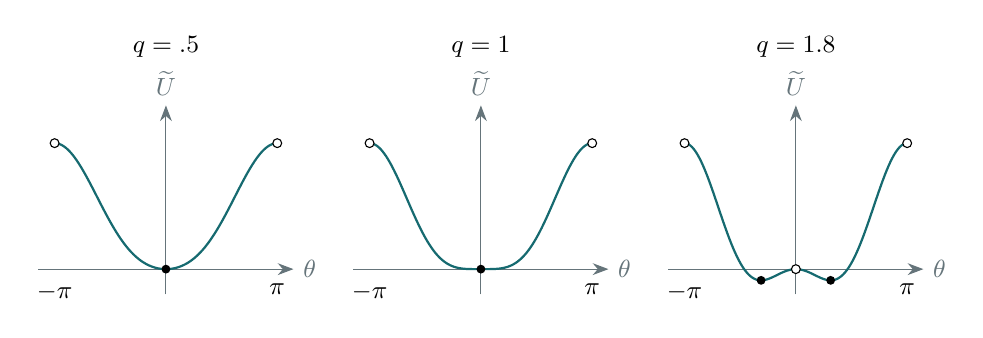
\begin{tikzpicture}
\foreach \q/\xx in {.5/0,1/4,1.8/8}{
\begin{scope}[xshift=\xx cm,x=.45cm,y=.8cm]
\draw[axis] (-3.6,0)--(3.6,0) node[right] {$\theta$};
\draw[axis] (0,-.4)--(0,2.6) node[above] {$\widetilde U$};
\draw[traj,domain=-pi:pi,samples=120] plot(\x,{1-cos(\x r)-\q/2*sin(\x r)^2});
\node[above] at (0,3.2) {$q=\q$};
\node[below] at (-pi,-.08) {$-\pi$};\node[below] at (pi,-.08) {$\pi$};
\draw[fill=white] (-pi,2) circle(1.6pt);\draw[fill=white] (pi,2) circle(1.6pt);
\ifdim\q pt>1pt
 \draw[fill=white] (0,0) circle(1.6pt);
 \pgfmathsetmacro{\te}{acos(1/\q)/180*pi}
 \pgfmathsetmacro{\ue}{1-1/\q-\q/2*(1-1/(\q*\q))}
 \fill (-\te,\ue) circle(1.6pt);\fill (\te,\ue) circle(1.6pt);
\else
 \fill (0,0) circle(1.6pt);
\fi
\end{scope}}
\end{tikzpicture}
\figcaption{解图3.13B\quad 实心点为稳定位置，空心点为不稳定位置；左右端的顶点属于同一周期位置。}
\end{minipage}\end{center}

临界转速下还可以不用截断级数，直接将有效势能化为
\[
U=mgR\left(1-\cos\theta-\frac12\sin^2\theta\right)
=\frac{mgR}{2}(1-\cos\theta)^2\geq0.
\]
底点仍是严格的势能极小点，附近的小扰动局限在这个势阱内。此时势能从四次项开始，回复力矩从三次项开始，线性振动频率为零。

若小摆幅为$A\ll1$，保留四次势能，回复方程为
$\ddot\theta\simeq-g\theta^3/(2R)$。
从$\theta=A$静止出发，用能量积分，
\[
\frac12mR^2\dot\theta^2
=\frac{mgR}{8}(A^4-\theta^4),\qquad
\dot\theta^2=\frac g{4R}(A^4-\theta^4).
\]
四分之一周期是从底点到最大偏角的积分，故最低阶周期为
\[
T(A)\simeq\frac{8}{A}\sqrt{\frac Rg}
\int_0^1\frac{\dd u}{\sqrt{1-u^4}}.
\]
最低阶周期与振幅 $A$ 成反比，振幅趋于零时周期趋于无穷。
这一结论与势能曲线在底点更平坦、线性频率为零相符。


\Needspace{18\baselineskip}

\pdfbookmark[2]{第 14 题 弹性小球与移动墙壁}{q14}

\section*{第 14 题\quad 弹性小球与移动墙壁}

\tagline{M-03-14}

质量为 $m$ 的小球在相距 $l$ 的两平行墙壁间，以垂直于墙壁的初速 $v_0$ 往返。墙质量远大于球，碰撞完全弹性，忽略其他作用。\begin{enumerate}\item 两墙固定时，求每壁所受平均力。\item 左壁以 $V\ll v_0$ 缓慢右移，证明在准静态极限中，外力对左壁所做的功等于小球动能增加量。\end{enumerate}

\begin{center}\begin{minipage}{\linewidth}\centering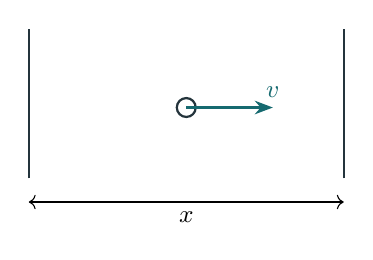
\begin{tikzpicture}
\draw[object](0,-.5)--(0,1.4);\draw[object](4,-.5)--(4,1.4);\filldraw[object,fill=white](2,.4)circle(.12);\draw[motion](2,.4)--(3.1,.4)node[above]{$v$};\draw[<->](0,-.8)--(4,-.8)node[midway,below]{$x$};
\end{tikzpicture}
\figcaption{图 3.14\quad 第二问中，壁距从 $l$ 缩短到 $x$。}
\end{minipage}\end{center}

\Needspace{5\baselineskip}\subsection*{解答}

固定壁每隔 $2l/v_0$ 受到一次大小为 $2mv_0$ 的冲量。移动左壁的碰撞在壁系中反向，解图 3.14A 给出地面系的速度变化。
\begin{center}\begin{minipage}{\linewidth}\centering\begin{tikzpicture}
\draw[object](0,-.5)--(0,1.4);\draw[object](4,-.5)--(4,1.4);\filldraw[object,fill=white](2,.4)circle(.12);\draw[motion](2,.4)--(3.1,.4)node[above]{$v$};\draw[<->](0,-.8)--(4,-.8)node[midway,below]{$x$};\draw[motion](0,1)--(.8,1)node[above]{$V$};\node[align=left]at(6,.6){撞左壁前：$-v$\\撞左壁后：$v+2V$\\一周速度增量：$2V$};
\end{tikzpicture}
\figcaption{解图 3.14A\quad 慢压缩极限中，球速与壁距的乘积保持不变。}
\end{minipage}\end{center}

\subsubsection*{固定墙所受平均力}
一次完全弹性碰撞中，球的动量由 $mv_0$ 变为 $-mv_0$，墙所受冲量大小为 $2mv_0$。
同一面墙的两次碰撞之间，球要去对面再返回，间隔为 $2l/v_0$，故
\[
\boxed{\overline F=\frac{2mv_0}{2l/v_0}=\frac{mv_0^2}{l}}.
\]
这里求完整往返周期内的冲量平均力。单次接触期间的瞬时力还取决于接触持续时间。

\subsubsection*{移动墙的单次速度变化}
左壁向右速度为 $V$，球撞它前向左的地面速度为 $-v$。进入墙系，球速度是 $-v-V$；完全弹性反弹后为 $v+V$；再加上墙速，地面速度变为
\[
v'=v+2V.
\]
解图3.14A 的碰前、碰后速度以墙速 $V$ 为中点。球到达固定的右壁时，反弹速度与入射速度大小相等、方向相反。

\subsubsection*{慢压缩的微分关系}
设这次往返开始时的壁距和球速分别为 $x,v$。在 $V/v\to0$ 的极限，往返中壁距和球速的相对改变量都趋于零，因此可用这两个起始值估计往返时间 $\Delta t\simeq2x/v$。相邻两次碰左壁之间，
\[
\Delta v=2V,\qquad \Delta x=-V\Delta t\simeq-\frac{2Vx}{v}.
\]
因此 $\dd v/\dd x=-v/x$，积分并使用初态，
\[
\ln(v/v_0)=-\ln(x/l),\qquad
\boxed{vx=v_0l}.
\]
每轮传给墙的冲量大小在慢变化极限中为 $2mv$，除以当时的往返时间 $2x/v$，得到慢压缩极限中的平均力，
\[
\overline F(x)=\frac{mv^2}{x}
=\frac{mv_0^2l^2}{x^3}.
\]
球对左壁平均作用向左，维持右移的外力向右；左壁向右的位移为 $-\dd x$，所以
\[
W=-\int_l^x\overline F(\xi)\,\dd\xi
=\frac12mv_0^2\left(\frac{l^2}{x^2}-1\right).
\]
再用 $v=v_0l/x$，
\[
\boxed{W=\frac12mv^2-\frac12mv_0^2}.
\]
两墙固定时，球的速率保持 $v_0$。左壁向右运动时，维持壁速的外力通过每次碰撞向球输送能量。壁距减半时，$vx=v_0l$ 给出球速加倍，动能增至初值的四倍，所需功等于三份初动能。$vx$ 和平均力关系适用于慢变化极限。单次碰撞的速度关系 $v'=v+2V$ 直接来自墙系的弹性反弹。
\subsubsection*{运动墙壁单次碰撞的冲量与能量传递}
在解图3.14A中，球碰左壁前的有符号速度为$-v$，碰后为$v+2V$。
对地面系的球应用冲量关系，动量增加为
\[
J=m[(v+2V)-(-v)]=2m(v+V).
\]
球对墙的冲量为$-J$。若外驱动维持墙速$V$不变，
外驱动在碰撞期间补偿的冲量就是$J$，其功为
\[
W_{\rm drive}=VJ=2mV(v+V)
=\frac12m(v+2V)^2-\frac12mv^2=\Delta K.
\]
固定右壁的作用点位移为零，它对球所做的功为零，碰撞冲量则改变球的动量方向。
将所有碰撞的动能增量相加，中间状态逐项抵消，外驱动总功等于球最终与初始动能之差。
每次碰撞的能量增量均由墙壁位移和冲量给出。采用慢压缩近似后，离散碰撞中的能量增加可进一步写成$v(x)$和平均力的连续函数。

解图3.14B把三个有符号速度放到同一数轴：
碰前、碰后速度相对墙速的距离相等，方向相反。
速度数轴上以墙速$V$为反射中心，两端点分别给出球碰前与碰后的地面速度。
\begin{center}\begin{minipage}{\linewidth}\centering
\begin{tikzpicture}
\draw[axis] (-3,0)--(4.1,0) node[right] {地面系速度};
\foreach \x/\lab in {-2/{-v},.5/{V},3/{v+2V}}{
 \fill (\x,0) circle(1.8pt);\node[below] at (\x,-.05) {$\lab$};}
\draw[guide] (.5,-.5)--(.5,1.4);
\draw[<->] (-2,.8)--(.5,.8) node[midway,above] {$v+V$};
\draw[<->] (.5,.8)--(3,.8) node[midway,above] {$v+V$};
\node[below] at (.5,-.62) {墙速为反射中心};
\end{tikzpicture}
\figcaption{解图3.14B\quad 先减墙速，再把相对速度反号，最后加回墙速；图上两段等长。}
\end{minipage}\end{center}


\Needspace{18\baselineskip}

\pdfbookmark[2]{第 15 题 三质点绳系冲量}{q15}

\section*{第 15 题\quad 三质点绳系冲量}

\tagline{M-03-15}

光滑水平面上，静止质点 $A,B,C$ 的质量分别为 $m_1,m_2,m_3$，用两段拉直的理想细绳相连。$\alpha$ 是 $A\to B$ 与 $B\to C$ 两方向的夹角，$0\leq\alpha<90^\circ$。沿 $B\to C$ 方向对 $C$ 施加冲量 $I$。求 $A$ 刚开始运动的速率。

\begin{center}\begin{minipage}{\linewidth}\centering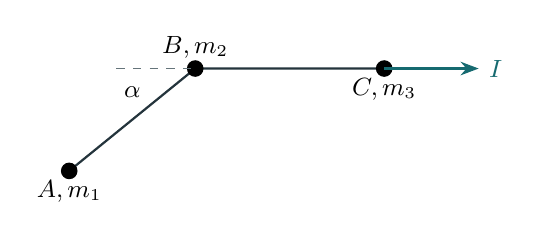
\begin{tikzpicture}
\coordinate(A)at(-1.6,-1.3);\coordinate(B)at(0,0);\coordinate(C)at(2.4,0);\draw[object](A)--(B)--(C);\fill(A)circle(3pt);\fill(B)circle(3pt);\fill(C)circle(3pt);\node[below]at(A){$A,m_1$};\node[above]at(B){$B,m_2$};\node[below]at(C){$C,m_3$};\draw[motion](C)--(3.6,0)node[right]{$I$};\draw[guide](-1,0)--(B);\node at(-.8,-.3){$\alpha$};
\end{tikzpicture}
\figcaption{图 3.15\quad 俯视图；夹角按两条有向绳段的方向定义。}
\end{minipage}\end{center}

\Needspace{5\baselineskip}\subsection*{解答}

解图 3.15A 以 $\vect e$ 沿 $A\to B$、$\vect f$ 沿 $B\to C$，令两绳张力冲量为 $P,Q$。瞬间几何位置不变，绳长约束作用在速度沿绳的投影上。
\begin{center}\begin{minipage}{\linewidth}\centering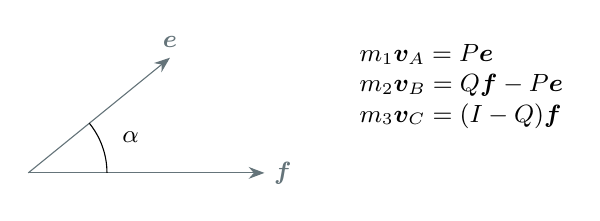
\begin{tikzpicture}
\draw[axis](0,0)--(3,0)node[right]{$\vect f$};\draw[axis](0,0)--(1.8,1.4625)node[above]{$\vect e$};\draw (1,0)arc(0:39.0939:1);\node at(1.3,.45){$\alpha$};\node[align=left]at(5.5,1.1){$m_1\vect v_A=P\vect e$\\$m_2\vect v_B=Q\vect f-P\vect e$\\$m_3\vect v_C=(I-Q)\vect f$};
\end{tikzpicture}
\figcaption{解图 3.15A\quad 两段绳各传递一个张力冲量。}
\end{minipage}\end{center}

\subsubsection*{冲量方程与方向}
定义 $\vect e$ 沿 $A\to B$，$\vect f$ 沿 $B\to C$，有 $\vect e\cdot\vect f=\cos\alpha$。两段绳的张力冲量分别记为 $P,Q$。位置在短冲量过程中来不及改变，故这两个单位方向可视为固定。
解图 3.15A 的三个动量定理为
\[
m_1\vect v_A=P\vect e,\quad
m_2\vect v_B=Q\vect f-P\vect e,\quad
m_3\vect v_C=(I-Q)\vect f.
\]
三式相加时，绳的内冲量成对抵消，系统总动量因而增加 $I\vect f$。

\subsubsection*{绳长约束与速度投影}
对 $AB$ 长度平方求导，得
$(\vect v_B-\vect v_A)\cdot\vect e=0$；对 $BC$ 同理。每条约束给出相邻两球沿这一绳段的速度分量。$B$ 同时受两绳的冲量，完整速度由两条方向的分量共同确定。将冲量式代入，得到
\[
\frac{Q\cos\alpha-P}{m_2}=\frac{P}{m_1},
\qquad
\frac{Q-P\cos\alpha}{m_2}=\frac{I-Q}{m_3}.
\]
由第一式，
\[
P=\frac{m_1Q\cos\alpha}{m_1+m_2}.
\]
代入第二式，乘以 $m_2m_3(m_1+m_2)$ 并整理，
\[
Q\left[m_2(m_1+m_2+m_3)+m_1m_3\sin^2\alpha\right]
=I m_2(m_1+m_2).
\]
因此 $v_A=P/m_1$ 为
\[
\boxed{v_A=
\frac{I m_2\cos\alpha}
{m_2(m_1+m_2+m_3)+m_1m_3\sin^2\alpha}}.
\]

\subsubsection*{两绳绷紧时的拉力冲量及夹角的极限}
题设 $0\leq\alpha<90^\circ$ 内，$Q>0,P>0$，两绳传递的确是拉力冲量。直线排列 $\alpha=0$ 时，式子化为三球同速 $I/(m_1+m_2+m_3)$；夹角趋于直角时，$P$ 趋于零，$A$ 在冲量结束时的速率也趋于零。

两绳绷紧的分支由拉力冲量$P,Q\ge0$确定。夹角扩展到钝角时，形式解的$P<0$对应第一段受压；细绳在这一阶段松弛，第一段拉力冲量取零后另列冲量方程。若第一段改成可受压的轻杆，该形式解对应杆的推力冲量。本题给定外冲量，各球的末速度由冲量方程与绳长约束共同确定，动能的变化则由这些末速度计算。
\subsubsection*{三球速度及沿绳的投影}
记解图3.15A联立式中的公共分母为
$D=m_2(m_1+m_2+m_3)+m_1m_3\sin^2\alpha>0$。
先由消元式求出两绳冲量，
\[
Q=\frac{I m_2(m_1+m_2)}D,
\qquad P=\frac{I m_1m_2\cos\alpha}D.
\]
因此三个速度矢量分别是
\[
\begin{aligned}
\vect v_A&=\frac{I m_2\cos\alpha}D\vect e,\\
\vect v_B&=\frac I D[(m_1+m_2)\vect f-m_1\cos\alpha\,\vect e],\\
\vect v_C&=\frac{I(m_2+m_1\sin^2\alpha)}D\vect f.
\end{aligned}
\]
$\vect v_B\cdot\vect f=I(m_2+m_1\sin^2\alpha)/D$
与$\vect v_C\cdot\vect f$相同；
$\vect v_B\cdot\vect e=I m_2\cos\alpha/D$
也与$\vect v_A\cdot\vect e$相同。
两项投影分别给出 $BC$ 和 $AB$ 两段绳的长度变化率均为零。$B$ 的完整速度由两个非平行的冲量相加得到。
三质量相等、$\alpha=60^\circ$时$D=15m^2/4$，
代入得$v_A=2I/(15m)$。分母 $D$ 的各项都有质量平方的量纲，分子 $I m_2$ 与它相除所得量纲为速度。


\Needspace{18\baselineskip}

\pdfbookmark[2]{第 16 题 炮弹最高点爆炸}{q16}

\section*{第 16 题\quad 炮弹最高点爆炸}

\tagline{M-03-16}

炮弹从地面发射，在最高点炸成质量相等的两块。最高点高 $h=19.6\,\mathrm m$，其正下方距发射点 $S_1=1000\,\mathrm m$。第一块在爆炸后 $1.00\,\mathrm s$ 落到该正下方点。忽略空气阻力，取 $g=9.8\,\mathrm{m/s^2}$，求第二块落地点距发射点的水平距离。

\begin{center}\begin{minipage}{\linewidth}\centering\begin{tikzpicture}
\draw[object](-.3,0)--(6,0);\draw[traj](0,0)..controls(.5,1.8)and(1.5,2.4)..(2.2,2.4);\draw[guide](2.2,2.4)--(2.2,0);\fill(2.2,2.4)circle(3pt);\node[above]at(2.2,2.4){爆炸点};\node[below]at(0,0){$O$};\node[below]at(2.2,0){$S_1$};\draw[<->](3,0)--(3,2.4)node[midway,right]{$h$};
\end{tikzpicture}
\figcaption{图 3.16\quad 图示不按水平与竖直距离的实际比例。}
\end{minipage}\end{center}

\Needspace{5\baselineskip}\subsection*{解答}

上升时间为 $t_a=\sqrt{2h/g}=2\,\mathrm s$，故最高点爆炸前水平速度为 $v=S_1/t_a=500\,\mathrm{m/s}$。解图 3.16A 对两块速度分别列水平、竖直动量。
\begin{center}\begin{minipage}{\linewidth}\centering\begin{tikzpicture}
\fill(0,1)circle(3pt);\draw[motion](0,1)--(1.2,1)node[above]{$v$};\draw[motion](0,1)--(0,-.4)node[below]{$v_{1y}=-14.7$};\draw[motion](0,1)--(2,2)node[right]{$\vect v_2=(1000,14.7)$};\node[align=left]at(5,1){两块质量相等\\$v_{1x}+v_{2x}=2v$\\$v_{1y}+v_{2y}=0$};
\end{tikzpicture}
\figcaption{解图 3.16A\quad 速度数字的单位为 $\mathrm{m/s}$。箭头示意各速度分量的方向。}
\end{minipage}\end{center}

\subsubsection*{最高点的速度}
炮弹到最高点时竖直速度为零。由上升高度，
\[
h=\frac12g t_a^2,\quad
t_a=\sqrt{\frac{2h}{g}}=2.00\,\mathrm s.
\]
水平速度一直不变，最高点水平位置为 $S_1$，所以
\[
v_x=\frac{S_1}{t_a}=500\,\mathrm{m/s}.
\]
爆炸前速度是 $(500,0)\,\mathrm{m/s}$。

\subsubsection*{第一块的落地条件}
以爆炸点正下方为水平坐标原点，竖直向上为正。第一块落在同一竖线上且无水平加速度，因此爆炸后 $v_{1x}=0$。它在 $\tau=1.00\,\mathrm s$ 后从高 $h$ 到达地面，
\[
0=h+v_{1y}\tau-\frac12g\tau^2.
\]
代入数值，得
\[
v_{1y}=\frac{-19.6+4.9}{1.00}
=-14.7\,\mathrm{m/s}.
\]
负号表示第一块在分离瞬间已有向下速度。这一初速度与重力加速度共同决定一秒内的竖直位移。

\subsubsection*{瞬时动量与第二块轨迹}
设炮弹总质量为 $M_p$。爆炸时间很短，外部重力冲量可忽略，两个方向都可用动量守恒。两块质量均为 $M_p/2$，故
\[
M_p(500)=\frac{M_p}{2}(0+v_{2x}),\qquad
0=\frac{M_p}{2}(v_{1y}+v_{2y}).
\]
得到
\[
v_{2x}=1000\,\mathrm{m/s},\qquad v_{2y}=+14.7\,\mathrm{m/s}.
\]
这与解图 3.16A 中向右上的速度箭头一致。第二块先继续上升，再下落，它的落地时间需单独求：
\[
0=19.6+14.7t_2-4.9t_2^2,\qquad
t_2^2-3t_2-4=0.
\]
两个代数根为 $4\,\mathrm s$ 和 $-1\,\mathrm s$。分离后的飞行取 $t_2>0$，故第二块飞行 $4\,\mathrm s$，其间的水平速度恒为 $v_{2x}$。落点距发射点为
\[
\boxed{S_2=1000+1000\times4=5000\,\mathrm m}.
\]
分离过程中，释放的内能使两块的总动能增加。分离后两块分别按各自的初速度运动。第一块触地前，系统合外力是总重力，质心延续未分离时的抛体运动。第一块触地后，地面的作用进入质心方程，后续质心轨迹由新的外力决定。
\subsubsection*{两块的位置与触地前的质心轨迹}
以爆炸瞬间为$\tau=0$，坐标原点仍放在发射点$O$，
解图3.16B中两块自由飞行时的坐标分别为
\[
\begin{aligned}
x_1&=1000,& y_1&=19.6-14.7\tau-4.9\tau^2,\\
x_2&=1000+1000\tau,& y_2&=19.6+14.7\tau-4.9\tau^2.
\end{aligned}
\]
这里长度用米、时间用秒。第一行描述第一块碎片在$0\leq\tau\leq1$的自由飞行，$\tau=1$时它首次触地，这一段抛物线到此结束。
由于质量相等，两块仍在空中时，质心坐标为
\[
x_{\rm cm}=1000+500\tau,
\qquad y_{\rm cm}=19.6-4.9\tau^2,
\quad 0\leq\tau\leq1.
\]
例如$\tau=0.5\,\mathrm s$时，质心位于$(1250,18.375)\,\mathrm m$，
与最高点以水平速度$500\,\mathrm{m/s}$继续飞行的未爆炸炮弹一致。
\begin{center}\begin{minipage}{\linewidth}\centering
\begin{tikzpicture}[x=1.3cm,y=1.5cm]
\draw[axis] (-1.5,0)--(4.65,0) node[right] {$(x-S_1)/(1000\,\mathrm m)$};
\draw[axis] (-1.3,-.1)--(-1.3,1.95) node[above] {$y/h$};
\draw[guide] (-1.3,1)--(0,1);\node[left] at (-1.3,1) {$1$};
\draw[thin,domain=-2:0,samples=50] plot({.5*\x},{1-.25*(\x)^2});
\draw[force,->] (0,1)--(0,0);
\draw[traj,domain=0:4,samples=100] plot(\x,{1+.75*\x-.25*\x^2});
\fill (0,1) circle(1.8pt);\node[above left] at (0,1) {爆炸点};
\fill (4,0) circle(1.8pt);\node[right] at (4.08,.34) {第二块：$\tau=4$};
\node[below] at (.18,-.18) {第一块：$\tau=1$};
\node[below] at (-1,-.05) {$O$};\node[above] at (2,1.5) {第二块先上升再下降};
\end{tikzpicture}
\figcaption{解图3.16B\quad 两碎片的实际飞行段；横、纵轴分别归一化，第一块的曲线在触地处停止。}
\end{minipage}\end{center}
从爆炸前的上升段还可反求发射竖直速度$v_{0y}=gt_a=19.6\,\mathrm{m/s}$。
若物体未分离，从最高点到地面经过 $2$ 秒，落在 $2000$ 米处。两个碎片的最终落点分别是 $1000$ 米和 $5000$ 米，平均值为 $3000$ 米。第一块与第二块分别在分离后 $1$ 秒和 $4$ 秒到达各自落点，质心坐标则须用同一时刻的两个位置求得。


\Needspace{18\baselineskip}

\pdfbookmark[2]{第 17 题 平板车上多人跳离}{q17}

\section*{第 17 题\quad 平板车上多人跳离}

\tagline{M-03-17}

光滑水平地面上，静止平板车质量为 $M$，载有 $N$ 人，每人质量为 $m$。每人向车后跳离，相对于该次跳离后车的速度大小均为 $u$。比较 $N$ 人同时跳离与逐个跳离后，车所得动能的大小。

\begin{center}\begin{minipage}{\linewidth}\centering\begin{tikzpicture}
\draw[object](0,.3)rectangle(4,.6);\draw[object](.6,.15)circle(.15);\draw[object](3.4,.15)circle(.15);\draw[object](-.5,0)--(5,0);\foreach\x in {.8,2,3.2}{\filldraw[object,fill=white](\x,1.1)circle(.15);\draw[object](\x,.95)--(\x,.6);}\node at(2,.43){$M$};\node[above]at(2,1.45){$N$ 人，每人 $m$};
\end{tikzpicture}
\figcaption{图 3.17\quad 向右取车前进的正方向。}
\end{minipage}\end{center}

\Needspace{5\baselineskip}\subsection*{解答}

解图 3.17A 中，向后相对速度为 $-u$，因此人的地面速度是跳后车速减 $u$。两种跳法都以同一个相对速率 $u$ 离开该次跳后的车。人体做功由各次跳前、跳后的总动能之差确定。
\begin{center}\begin{minipage}{\linewidth}\centering\begin{tikzpicture}
\draw[object](0,.3)rectangle(4,.6);\draw[object](.6,.15)circle(.15);\draw[object](3.4,.15)circle(.15);\draw[object](-.5,0)--(5,0);\foreach\x in {.8,2,3.2}{\filldraw[object,fill=white](\x,1.1)circle(.15);\draw[object](\x,.95)--(\x,.6);}\node at(2,.43){$M$};\node[above]at(2,1.45){$N$ 人，每人 $m$};\draw[motion](4,.7)--(5.3,.7)node[right]{$V$};\draw[motion](-.3,1.2)--(-1.6,1.2)node[left]{$u$（相对车）};\node at(2,2.55){人：$V-u$，车：$V$};
\end{tikzpicture}
\figcaption{解图 3.17A\quad 人向后跳离时，地面速度为$V-u$；$u$相对于该次跳离后的车定义。}
\end{minipage}\end{center}

\subsubsection*{同时跳离}
向右取正，车最终速度为 $V_{\mathrm{sim}}$。人相对跳后车向左的速率为 $u$，因此人的地面速度是 $V_{\mathrm{sim}}-u$，由车速与向后的相对速度相加得到。水平无外力，
\[
0=MV_{\mathrm{sim}}+Nm(V_{\mathrm{sim}}-u).
\]
所以
\[
\boxed{V_{\mathrm{sim}}=\frac{Nmu}{M+Nm}},\qquad
K_{\mathrm{sim}}=\frac12M V_{\mathrm{sim}}^2.
\]
解图 3.17A 的速度标注须按这一相对关系读取。

\subsubsection*{逐个跳离的递推}
令第 $j$ 人跳离后车速为 $V_j$，$V_0=0$。该次跳前仍在车上的人数为 $N-j+1$，全都以 $V_{j-1}$ 运动。跳后剩余车人总质量为 $M+(N-j)m$，跳离者地面速度为 $V_j-u$。
只对本次参加相互作用的人和剩余车人系统列动量守恒：
\[
[M+(N-j+1)m]V_{j-1}
=[M+(N-j)m]V_j+m(V_j-u).
\]
合并右侧，
\[
\boxed{V_j-V_{j-1}
=\frac{mu}{M+(N-j+1)m}}.
\]
把 $N$ 次增量相加，再以 $k=N-j+1$ 换指标，得到
\[
\boxed{V_{\mathrm{seq}}=mu\sum_{k=1}^{N}\frac1{M+km}}.
\]
已经离车的人保持各自的地面速度。递推式的两边都只计这一次相互作用的跳离者与剩余车人。

\subsubsection*{比较速度与动能}
和式的每项分母都不大于 $M+Nm$，故
\[
\sum_{k=1}^{N}\frac1{M+km}
\geq\frac{N}{M+Nm}.
\]
$N>1$ 时至少有一个分母严格较小，速度与动能均有严格不等式：
\[
\boxed{V_{\mathrm{seq}}>V_{\mathrm{sim}},\qquad
K_{\mathrm{seq}}>K_{\mathrm{sim}}}.
\]
$N=1$ 时两者相同。以 $N=2$ 为例，两次增量分别为 $mu/(M+2m)$、$mu/(M+m)$；第二个人推动的剩余质量较少，车的速度增量较大。
上述比较以每次相对跳速相同为条件。两种跳法的人和车最终速度不同，总机械功可由各自末态的总动能另算。
\subsubsection*{先把前两次跳离的计算展开}
第一人跳离前总动量为零，故
\[
0=[M+(N-1)m]V_1+m(V_1-u),
\qquad V_1=\frac{mu}{M+Nm}.
\]
第二次只选剩余车人作为本次相互作用系统，其跳前总动量为
$[M+(N-1)m]V_1$，因此
\[
[M+(N-1)m]V_1=[M+(N-2)m]V_2+m(V_2-u).
\]
合并$V_2$的系数，解得
\[
V_2=\frac{mu}{M+Nm}+\frac{mu}{M+(N-1)m}.
\]
从第一步到第二步，参与动量分配的总质量少了 $m$。以后每步再少一个人的质量，把这些速度增量相加即为前面的有限和。

例如$N=2,M=m$，同时跳离给$V_{\rm sim}=2u/3$，
逐个跳离给$V_{\rm seq}=u/3+u/2=5u/6$，车动能之比为$25/16$。
逐个跳时两人的最终地速分别为$-2u/3$、$-u/6$；
连同车速$5u/6$加权相加，总动量仍为零。
三者最终总动能为$7mu^2/12$，同时跳的总动能为$mu^2/3$，
在这个例子中，逐个跳离使车获得的动能增加，同时也需要较大的输入机械功。


\Needspace{18\baselineskip}

\pdfbookmark[2]{第 18 题 下滑木块中支持力做功}{q18}

\section*{第 18 题\quad 下滑木块中支持力做功}

\tagline{M-03-18}

质量 $M$、倾角 $\theta$ 的斜面体放在光滑水平地面上，质量 $m$ 的木块从斜面顶端高 $h$ 处静止滑至底端。块与斜面之间也光滑。以地面为参考系，求斜面支持力对木块做的功。

\begin{center}\begin{minipage}{\linewidth}\centering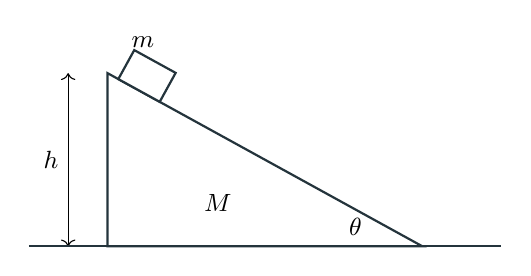
\begin{tikzpicture}
\draw[object](0,0)--(4,0)--(0,2.2)--cycle;\filldraw[object,fill=white,rotate around={-28.81:(.4,1.98)}](.1,1.98)rectangle(.7,2.4);\node at(1.4,.55){$M$};\node[above]at(.45,2.4){$m$};\draw[<->](-.5,0)--(-.5,2.2)node[midway,left]{$h$};\draw[object](-1,0)--(5,0);\node at(3.15,.25){$\theta$};
\end{tikzpicture}
\figcaption{图 3.18\quad 木块相对斜面向右下滑，斜面向左移动。}
\end{minipage}\end{center}

\Needspace{5\baselineskip}\subsection*{解答}

设木块相对斜面的速率为 $w$，斜面向左速率为 $U$。解图 3.18A 分解木块的地面速度；斜面向左的速度分量使木块的实际位移在支持力方向上出现负投影。
\begin{center}\begin{minipage}{\linewidth}\centering\begin{tikzpicture}
\draw[motion](0,0)--(2,-1.1)node[right]{$\vect w$};\draw[motion](0,0)--(-1,0)node[left]{$-U\vect e_x$};\draw[motion](0,0)--(1,-1.1)node[below]{$\vect v$};\draw[guide](-1,0)--(1,-1.1)--(2,-1.1);\draw[force](0,0)--(.7,1.272727)node[above]{$N$};\node[align=left]at(5,0){$v_x=w\cos\theta-U$\\$v_y=-w\sin\theta$};
\end{tikzpicture}
\figcaption{解图 3.18A\quad 木块速度为相对滑动速度与斜面平动速度之和。}
\end{minipage}\end{center}

\subsubsection*{木块的地面速度}
设木块相对斜面向右下的速率为 $w$，斜面向左的速率为 $U>0$。解图 3.18A 的速度三角形给出
\[
v_x=w\cos\theta-U,\qquad v_y=-w\sin\theta.
\]
地面对斜面的支持力竖直，系统水平无外力，因此
\[
mv_x-MU=0,\qquad
\boxed{U=\frac{m}{M+m}w\cos\theta}.
\]
把该式代回，可得 $v_x=Mw\cos\theta/(M+m)$。

\subsubsection*{由整体能量确定速率}
木块下降 $h$，重力势能减小 $mgh$。接触无摩擦，地面的竖直支持力不做功，系统总能量守恒：
\[
mgh=\frac12m\left[(w\cos\theta-U)^2+w^2\sin^2\theta\right]
+\frac12MU^2.
\]
代入动量关系并合并平方项，
\[
mgh=\frac12m w^2
\left[\sin^2\theta+\frac{M}{M+m}\cos^2\theta\right].
\]
括号为 $(M+m\sin^2\theta)/(M+m)$，所以
\[
w^2=\frac{2gh(M+m)}{M+m\sin^2\theta}.
\]

\subsubsection*{支持力对谁做功}
对木块单独用动能定理，$K_m=mgh+W_N$。再与整体能量 $mgh=K_m+MU^2/2$ 比较，立即得到
\[
W_N=-\frac12MU^2.
\]
代入 $U$、$w$，
\[
\boxed{W_N=
-\frac{Mm^2gh\cos^2\theta}
{(M+m)(M+m\sin^2\theta)}}.
\]
负功大小等于斜面所得动能。支持力把一部分重力势能从木块传给斜面。两接触力的功大小相等、符号相反。

也可从瞬时功率解释符号。支持力方向为
$\vect n=(\sin\theta,\cos\theta)$，相对下滑速度垂直于它，所以
\[
N\vect n\cdot\vect v
=N\vect n\cdot(-U\vect e_x)=-NU\sin\theta<0.
\]
\subsubsection*{由支持力和实际位移直接积分}
同一结论还可从牛顿方程与位移求出。设斜面向左的加速度大小为 $a_M$，木块相对斜面的沿坡加速度为 $a_w$。分别投影，
\[
Ma_M=N\sin\theta,\qquad
a_w=g\sin\theta+a_M\cos\theta,
\]
\[
N-mg\cos\theta=-ma_M\sin\theta.
\]
消去 $N$，得到恒定的
\[
a_M=\frac{mg\sin\theta\cos\theta}{M+m\sin^2\theta},\qquad
N=\frac{mMg\cos\theta}{M+m\sin^2\theta}.
\]
木块相对斜面的水平位移为 $h\cot\theta$。设斜面左移距离为 $X>0$，系统水平质心不移动，故
\[
m(h\cot\theta-X)-MX=0,\qquad
X=\frac{mh\cot\theta}{M+m}.
\]
木块的地面位移是 $\Delta\vect r=(h\cot\theta-X,-h)$，于是
\[
\begin{aligned}
W_N&=N\vect n\cdot\Delta\vect r
=N[(h\cot\theta-X)\sin\theta-h\cos\theta]\\
&=-NX\sin\theta=-Ma_MX=-\frac12MU^2,
\end{aligned}
\]
其中最后一步使用从静止开始的 $U^2=2a_MX$。相对位移与支持力垂直，而地面位移多出斜面的平移，使支持力对滑块做负功。斜面固定的极限 $M\to\infty$ 中 $U\to0$，支持力功也趋零。
\subsubsection*{在位移图上直接看支持力负功}
解图3.18B用$AB$表示把斜面固定时的相对下滑路径，
用$AB'$表示木块在地面系中的实际路径。
末态斜面向左移$X$，因此$B'$在$B$左侧，
实际位移少了向右的$X\vect e_x$。
由于本题初态静止，且加速度的两个分量恒定，木块的地面轨迹也是直线。相比 $AB$，$AB^{\prime}$ 在相同下降高度下的水平跨度较小，向下的倾角较大。
\begin{center}\begin{minipage}{\linewidth}\centering
\begin{tikzpicture}
\coordinate(A)at(0,2.2);\coordinate(B)at(4,0);\coordinate(Ap)at(-.8,2.2);\coordinate(Bp)at(3.2,0);
\draw[object] (-1.2,0)--(4.6,0);
\draw[guide] (A)--(B)--(0,0)--cycle;
\draw[object] (Ap)--(Bp)--(-.8,0)--cycle;
\draw[traj] (A)--(B);
\draw[motion,line width=1.1pt] (A)--(Bp);
\draw[force] (1,1.5125)--(1.5,2.4216) node[above] {$N$};
\fill (A) circle(1.6pt);\fill (Bp) circle(1.6pt);
\node[above left] at (A) {$A$};\node[above left] at (Ap) {$A'$};
\node[below] at (B) {$B$};\node[below] at (Bp) {$B'$};
\draw[<->] (3.2,-.5)--(4,-.5) node[midway,below] {$X$};
\node[align=left,anchor=west] at (5,1.8) {$AB$：相对下滑位移\\$AB'$：地面位移\\
$\Delta\vect r=h(\cot\theta,-1)-X\vect e_x$\\
$\vect n\cdot\Delta\vect r=-X\sin\theta$};
\end{tikzpicture}
\figcaption{解图3.18B\quad 两末端相差斜面的平移；支持力垂直$AB$，却对$AB'$有负的位移投影。}
\end{minipage}\end{center}
两接触力的功相抵，还可逐时刻证明。
令斜面速度为$\vect V_M=-U\vect e_x$，木块对斜面的力为$-N\vect n$。
两力总功率为
\[
P_m+P_M=N\vect n\cdot\vect v-N\vect n\cdot\vect V_M
=N\vect n\cdot(\vect v-\vect V_M)
=N\vect n\cdot\vect w=0.
\]
接触双方沿法线的速度相同，所以相对速度只沿坡面。地面系中，两接触力分别对木块做负功、对斜面做等量正功，合起来没有能量耗散。若改用随斜面加速的参考系，木块位移沿坡面，支持力的功为零。该参考系的动能定理同时包含水平惯性力的功。


\Needspace{18\baselineskip}

\pdfbookmark[2]{第 19 题 半圆槽中小球与木块}{q19}

\section*{第 19 题\quad 半圆槽中小球与木块}

\tagline{M-03-19}

质量 $M$ 的木块放在光滑水平地面上，其上部有半径 $R$ 的光滑半圆凹槽。质量 $m$ 的小球从凹槽右侧最高边缘静止下滑。$\theta$ 为槽心到球的半径与向下竖直方向的夹角，$0\leq\theta\leq\pi/2$。求球的地面速率 $v$、木块向右速率 $V$、球相对槽速率 $w$ 的位置函数；再求球在最低点对槽的压力。

\begin{center}\begin{minipage}{\linewidth}\centering\begin{tikzpicture}
\draw[object](-2,1.7)--(-2,-.35)--(2,-.35)--(2,1.7);\draw[object](-1.7,1.7)arc(180:360:1.7);\draw[object](-2,1.7)--(-1.7,1.7);\draw[object](1.7,1.7)--(2,1.7);\filldraw[object,fill=white](1.7,1.7)circle(.1);\node[right]at(1.9,1.8){$m$};\node at(0,-.2){$M$};\draw[guide](0,1.7)--(0,0);\node[left]at(0,.9){$R$};
\end{tikzpicture}
\figcaption{图 3.19\quad 球从右缘沿凹槽向左下滑。}
\end{minipage}\end{center}

\Needspace{5\baselineskip}\subsection*{解答}

如解图 3.19A，球的相对速度向左下方，分量为 $(-w\cos\theta,-w\sin\theta)$；槽以速度 $V$ 向右。
\begin{center}\begin{minipage}{\linewidth}\centering\begin{tikzpicture}
\draw[object](-2,1.7)--(-2,-.35)--(2,-.35)--(2,1.7);\draw[object](-1.7,1.7)arc(180:360:1.7);\draw[object](-2,1.7)--(-1.7,1.7);\draw[object](1.7,1.7)--(2,1.7);\draw[guide](1.7,1.7)circle(.1);\node[above right]at(1.8,1.8){初态};\node at(0,-.2){$M$};\draw[guide](0,1.7)--(0,0);\node[left]at(0,.9){$R$};\draw[guide](0,1.7)--(1.2,.5);\filldraw[object,fill=white](1.2,.5)circle(.1);\node[above right] at(1.3,.6){$m$};\draw[motion](1.2,.5)--(.6,-.1)node[midway,above left]{$w$};\draw[motion](1.2,.5)--(2.1,.5)node[right]{$V$};\node at(.38,1){$\theta$};
\end{tikzpicture}
\figcaption{解图 3.19A\quad 小球的相对速度$\boldsymbol w$沿槽切线，车速$\boldsymbol V$沿水平，地面速度由两者相加。}
\end{minipage}\end{center}

\subsubsection*{分量关系和水平动量}
球从右缘向左下滑，球心相对槽心的位置是
$(R\sin\theta,-R\cos\theta)$。上图中的 $\theta$ 从 $\pi/2$ 减至零，相对速率 $w=-R\dot\theta>0$，其分量为
\[
v_{x,\mathrm{rel}}=-w\cos\theta,\quad
v_{y,\mathrm{rel}}=-w\sin\theta.
\]
木块向右速度为 $V$，故地面分量为
$v_x=V-w\cos\theta,v_y=-w\sin\theta$。系统初始水平动量为零，
\[
m(V-w\cos\theta)+MV=0,
\qquad \boxed{V=\frac{m\cos\theta}{M+m}w}.
\]
因此 $v_x=-Mw\cos\theta/(M+m)$，球在地面系也向左运动。

\subsubsection*{势能如何分给两物体}
球从边缘下降 $R\cos\theta$，故
\[
mgR\cos\theta=\frac12m(v_x^2+v_y^2)+\frac12MV^2.
\]
消去 $V$ 后，
\[
mgR\cos\theta
=\frac12m w^2\left(1-\frac{m}{M+m}\cos^2\theta\right).
\]
记 $D=1-m\cos^2\theta/(M+m)>0$，得到
\[
\boxed{w=\sqrt{\frac{2gR\cos\theta}{D}}},\qquad
\boxed{V=\frac{m\cos\theta}{M+m}w},
\]
\[
\boxed{v=w\sqrt{\sin^2\theta+
\left(\frac{M}{M+m}\right)^2\cos^2\theta}}.
\]
能量式中，两项平动动能分别取球和槽的地面速率。相对速率 $w$ 通过解图3.19A 的速度分解进入两项。

\subsubsection*{最低点压力使用相对曲率速度}
最低点 $\theta=0$ 时，
\[
w_b^2=\frac{2gR(M+m)}{M},\quad
V_b=\frac{m}{M+m}w_b,\quad
v_b=\frac{M}{M+m}w_b.
\]
槽只作水平平移，不具有竖直加速度；球在最低点的相对切向速度水平，竖直曲率加速度向上，大小为 $w_b^2/R$。
由球的竖直坐标 $y=-R\cos\theta$ 连续求两次时间导数，得到
$\ddot y=R\cos\theta\,\dot\theta^2+R\sin\theta\,\ddot\theta$，在最低点恰为 $w_b^2/R$。
于是
\[
N-mg=\frac{mw_b^2}{R},\qquad
\boxed{N=mg\left(3+\frac{2m}{M}\right)}.
\]
按第三定律，这也是球对槽的向下压力大小。槽分得一部分动能，所以球在地面系的速率小于固定槽时的值。到最低点时球与槽水平反向运动，球的相对速率因而较大，压力也大于固定槽的 $3mg$。令 $M\to\infty$，三个速度式与压力均退化为固定槽结果。
\subsubsection*{把三个速度写成独立的显式函数}
令$c=\cos\theta$，用有质量量纲的分母
$D_0=M+m-mc^2=M+m\sin^2\theta>0$。
从前面的速度与动量关系可依次写成
\[
\begin{aligned}
w^2&=\frac{2gRc(M+m)}{D_0},\\
V^2&=\frac{m^2c^2}{(M+m)^2}w^2
=\frac{2gRm^2c^3}{(M+m)D_0},\\
v^2&=\left[1-\frac{m(2M+m)}{(M+m)^2}c^2\right]w^2\\
&=\frac{2gRc[(M+m)^2-m(2M+m)c^2]}{(M+m)D_0}.
\end{aligned}
\]
题目所求三个速率取以上非负平方根。
由于$0\leq c\leq1$，第三式的方括号分子不小于$M^2>0$，
分母又不小于$M(M+m)>0$，所以整个下滑区间没有速度表达式的奇点。
在初始边缘$c=0$，三个速率都为零；到最低点$c=1$，
所得式子分别退回前面的$w_b,V_b,v_b$。

\subsubsection*{一般位置的径向方程与最低点的特殊性}
令槽向右加速度为$A_M$。解图3.19B采用随槽平移的参考系，
球除重力与支持力外还要计入水平向左的惯性力$-mA_M\vect e_x$。
指向槽心的单位向量为$(-\sin\theta,\cos\theta)$，故
\[
N-mg\cos\theta+mA_M\sin\theta=\frac{mw^2}{R}.
\]
槽受球的水平反作用力向右，$MA_M=N\sin\theta$。
消去加速度，得到
\[
N=\frac{mM(g\cos\theta+w^2/R)}{M+m\sin^2\theta}\geq0.
\]
释放处 $\theta=\pi/2$ 时支持力为零，随后 $\cos\theta>0$，支持力为正，小球沿槽面下滑。
最低点时$\sin\theta=0$，所以槽的水平加速度为零，
惯性力也为零，径向式便化为$N-mg=mw_b^2/R$。槽此时仍以 $V_b$ 向右运动，因接触力在这一瞬间竖直，水平速度的瞬时变化率为零。
\begin{center}\begin{minipage}{\linewidth}\centering
\begin{tikzpicture}
\filldraw[object,fill=white] (0,0) circle(.09);
\draw[force] (0,0)--(-.9,.9) node[above] {$N$};
\draw[force] (0,0)--(0,-1.2) node[right] {$mg$};
\draw[force,dashed] (0,0)--(-1.5,0) node[left] {$-mA_M\vect e_x$};
\draw[motion] (0,0)--(-.7,-.7) node[below left] {$w$};
\node at (-.3,1.6) {一般位置，随槽系};
\filldraw[object,fill=white] (5,0) circle(.09);
\draw[force] (5,0)--(5,1.2) node[right] {$N$};
\draw[force] (5,0)--(5,-1.2) node[right] {$mg$};
\draw[motion] (5,0)--(3.7,0) node[left] {$w_b$};
\node at (5,1.6) {最低点：$A_M=0$};
\node at (2.2,-1.8) {随槽系的径向加速度用$w^2/R$，不是地面速率$v^2/R$};
\end{tikzpicture}
\figcaption{解图3.19B\quad 一般位置须保留槽加速带来的惯性力；最低点该项恰好消失。}
\end{minipage}\end{center}


\Needspace{18\baselineskip}

\pdfbookmark[2]{第 20 题 非弹性碰撞后弹簧带起木块}{q20}

\section*{第 20 题\quad 非弹性碰撞后弹簧带起木块}

\tagline{M-03-20}

地面上的木块 $m_3$ 通过劲度系数 $k$ 的竖直轻弹簧连接上方木块 $m_2$，初始静止平衡。小球 $m_1$ 从距 $m_2$ 高 $h$ 处静止落下，与 $m_2$ 完全非弹性碰撞并粘住。求使反弹过程中弹簧拉力恰好达到 $m_3g$（离地临界）的最小 $h$。

\begin{center}\begin{minipage}{\linewidth}\centering\begin{tikzpicture}
\draw[object](-1,0)--(1,0);\filldraw[object,fill=white](-.5,0)rectangle(.5,.5);\node at(0,.25){$m_3$};\draw[object](0,.5)--(0,.7)--(-.2,.85)--(.2,1.05)--(-.2,1.25)--(.2,1.45)--(0,1.6);\filldraw[object,fill=white](-.5,1.6)rectangle(.5,2.1);\node at(0,1.85){$m_2$};\filldraw[object,fill=white](0,3.2)circle(.12);\node[right]at(.2,3.2){$m_1$};\draw[<->](1,2.1)--(1,3.2)node[midway,right]{$h$};
\end{tikzpicture}
\figcaption{图 3.20\quad 初始弹簧压缩量为 $m_2g/k$。}
\end{minipage}\end{center}

\Needspace{5\baselineskip}\subsection*{解答}

碰撞很短，只对 $m_1,m_2$ 用动量守恒。反弹阶段，在到达离地临界之前 $m_3$ 不动；解图 3.20A 用弹簧原长位置统一描述压缩和伸长。
\begin{center}\begin{minipage}{\linewidth}\centering\begin{tikzpicture}
\draw[axis](0,-1.6)--(0,2)node[above]{$y$};\draw[guide](-.8,0)--(3,0);\draw[guide](-.8,-1)--(3,-1);\draw[guide](-.8,1.3)--(3,1.3);\node[right]at(3,0){原长};\node[right]at(3,-1){$y_i=-m_2g/k$};\node[right]at(3,1.3){$y_c=m_3g/k$};\draw[motion](1,-.8)--(1,1.1)node[midway,left]{反弹};
\end{tikzpicture}
\figcaption{解图 3.20A\quad 临界状态在上方转折点，粘连体的速度为零。}
\end{minipage}\end{center}

\subsubsection*{碰撞前速率与碰后共同速率}
初始上木块的重力由弹簧支持，因此压缩量为
$x_0=m_2g/k$。小球自由下落至碰撞前，速率为 $u=\sqrt{2gh}$。
碰撞时间很短，弹簧长度尚未改变，有限的弹簧力与重力的冲量可忽略。只对小球与上木块列竖直动量守恒：
\[
m_1u=(m_1+m_2)v.
\]
记 $s=m_1+m_2$，碰后向下共同速率为
\[
v=\frac{m_1}{s}\sqrt{2gh}.
\]
完全非弹性碰撞使小球和上木块的一部分动能转化为内能。后续弹簧运动从刚求出的共同速度开始。

\subsubsection*{下木块离地的条件}
在下木块还静止时，若弹簧伸长 $y>0$，它对下木块向上拉力为 $ky$。地面支持力为 $N_g=m_3g-ky$，所以离地阈值伸长
\[
y_c=\frac{m_3g}{k}=x_c.
\]
解图 3.20A 中，粘连体从碰后位置 $y_i=-x_0$ 到临界位置 $y_c=x_c$，实际上升高度为 $x_0+x_c$。这段高度从弹簧压缩时的位置量到伸长 $x_c$ 的位置。

\subsubsection*{最小落高对应上转折点}
在 $y\geq0$ 区间，粘连体势能
$U(y)=ky^2/2+sgy$ 单调增加。恰能到达 $x_c$ 的最小能量，对应到达时速率为零；在达到阈值之前，下木块不动，约束力不做功。因此碰后机械能守恒给出
\[
\frac12sv^2+\frac12kx_0^2
=\frac12kx_c^2+sg(x_0+x_c).
\]
代入 $v,x_0,x_c$，
\[
\frac{m_1^2gh}{s}
=\frac{(m_3^2-m_2^2)g^2}{2k}
+\frac{s(m_2+m_3)g^2}{k}.
\]
右边提取 $(m_2+m_3)g^2/(2k)$，剩余因子为
$m_3-m_2+2s=2m_1+m_2+m_3$。故
\[
\boxed{h_c=
\frac{(m_1+m_2)(m_2+m_3)(2m_1+m_2+m_3)g}
{2km_1^2}}.
\]
等号时，零地面支持力只在上转折点出现，系统随即回落；它给出离地临界。当 $h>h_c$ 时，上部粘连体以正的向上速度到达这一伸长，弹簧拉力继续增大，下木块随之离地。到达阈值前，地面为下木块提供竖直支持。
\subsubsection*{新平衡位置、振幅与临界上转折点}
碰后粘连质量为$s=m_1+m_2$，下木块尚未移动。
仍用解图3.20A的向上坐标$y$，粘连体的新平衡位置为
$y_e=-sg/k$，角频率$\omega=\sqrt{k/s}$。
碰撞瞬间位置没有改变，所以
\[
\xi_i=y_i-y_e=-\frac{m_2g}{k}+\frac{sg}{k}
=\frac{m_1g}{k},\qquad \dot\xi_i=-v.
\]
碰撞发生在新平衡点上方。小球下落带来的动量使粘连体从这个位置向下运动。
振动能量给出
\[
A^2=\xi_i^2+\frac{v^2}{\omega^2}
=\frac{m_1^2g^2}{k^2}+\frac{2m_1^2gh}{sk}.
\]
上转折点为$y_{\max}=y_e+A$。
恰到离地阈值$y_c=m_3g/k$时，所需振幅为
$A_c=(s+m_3)g/k$，于是
\[
h_c=\frac{sg}{2km_1^2}[(s+m_3)^2-m_1^2].
\]
将平方差分解，
$(s+m_3-m_1)(s+m_3+m_1)
=(m_2+m_3)(2m_1+m_2+m_3)$，
便恢复前面的临界落高。振幅法和直接比较两个位置的能量使用了同一碰后初态。

碰撞时弹簧长度来不及改变。碰前小球的动能与碰后粘连体的动能之差，就是碰撞损失。
碰前小球动能为$m_1gh$，碰后可用动能为$m_1^2gh/s$，差值
\[
\Delta E_{\rm loss}=m_1gh-\frac{m_1^2gh}{s}
=\frac{m_1m_2}{m_1+m_2}gh>0.
\]
碰撞期间弹簧位置不变，所以它的势能没有参与这一步损失。
随后弹簧阶段以剩余的碰后动能为初值，才能同时保留碰撞的动量条件与振动的机械能守恒。


\Needspace{18\baselineskip}

\pdfbookmark[2]{第 21 题 滑块弹簧与断绳条件}{q21}

\section*{第 21 题\quad 滑块弹簧与断绳条件}

\tagline{M-03-21}

质量 $M$ 的长滑块静置于光滑水平面，右端用最大承受拉力为 $T_0$ 的理想绳系在墙上，左端固定劲度系数 $k$ 的轻弹簧。质量 $m$ 的小物以向左初速 $v_0$ 在滑块上无摩擦运动，压缩弹簧。约定绳张力达到 $T_0$ 即断裂，断裂本身不消耗能量。求：\begin{enumerate}\item 断绳的最小 $v_0$；\item 断绳后滑块的最大加速度；\item 小物脱离弹簧后，相对桌面的速度为零的条件。\end{enumerate}

\begin{center}\begin{minipage}{\linewidth}\centering\begin{tikzpicture}
\draw[object](0,0)rectangle(4,.35);\draw[object](0,.35)--(0,1.1);\draw[object](0,.7)--(.3,.7)--(.5,.85)--(.7,.55)--(.9,.85)--(1.1,.55)--(1.3,.7)--(1.8,.7);\filldraw[object,fill=white](2.8,.35)rectangle(3.4,.9);\node at(3.1,.62){$m$};\node at(2,.17){$M$};\draw[object](4,.17)--(5.2,.17);\draw[object](5.2,-.2)--(5.2,1.2);\node[above]at(4.6,.17){$T_0$};\draw[motion](3.4,1.3)--(2.3,1.3)node[left]{$v_0$};
\end{tikzpicture}
\figcaption{图 3.21\quad 弹簧接触只在压缩阶段存在，小物反弹到原长后离开。}
\end{minipage}\end{center}

\Needspace{5\baselineskip}\subsection*{解答}

断绳前滑块固定；断绳后水平动量才守恒。解图 3.21A 将这两个阶段分开，取向左为正方向。
\begin{center}\begin{minipage}{\linewidth}\centering\begin{tikzpicture}
\node[draw,rounded corners,align=left,text width=4.1cm]at(0,0){断绳瞬间\\$x_0=T_0/k$\\滑块速度 $0$\\小物速度 $v_1$};\draw[motion](2.3,0)--(3.4,0);\node[draw,rounded corners,align=left,text width=4.4cm]at(5.9,0){最大压缩\\两物体同速 $V$\\$m v_1=(M+m)V$\\最大力 $kx_{\max}$};
\end{tikzpicture}
\figcaption{解图 3.21A\quad 最大弹簧力出现在相对速度为零时。}
\end{minipage}\end{center}

\subsubsection*{断绳前：滑块固定}
取小物向左运动为正，弹簧压缩量为 $x$。绳把长滑块固定，故绳张力等于弹簧对滑块的力 $kx$。断绳条件是 $kx_0=T_0$，即 $x_0=T_0/k$。
断绳前，小物与弹簧的机械能守恒：
\[
\frac12mv_0^2=\frac12mv_1^2+\frac12kx_0^2.
\]
达到 $x_0$ 时，小物的动能为初动能减去 $kx_0^2/2$；取这份动能恰为零给出临界初速：
\[
\boxed{v_{0,\min}=\frac{T_0}{\sqrt{mk}}},\qquad
v_1=\sqrt{v_0^2-\frac{T_0^2}{mk}}.
\]
固定绳在这一阶段改变系统的水平动量。绳在滑块上的系点静止，绳力的功为零。

\subsubsection*{断绳后：最大压缩和最大加速度}
断绳后，系统水平无外力，总动量固定为 $mv_1$。最大压缩对应相对速度零，即两物体同速
\[
V=\frac{mv_1}{M+m}.
\]
如解图 3.21A，弹簧力随压缩增加，故滑块最大加速度出现在这一时刻。断裂不损失能量，全程可用
\[
\frac12mv_0^2=\frac12(M+m)V^2+\frac12kx_{\max}^2.
\]
代入 $V,v_1$，
\[
kx_{\max}^2
=mv_0^2-\frac{m^2}{M+m}
\left(v_0^2-\frac{T_0^2}{mk}\right)
=\frac{mM}{M+m}v_0^2+\frac{mT_0^2}{k(M+m)}.
\]
于是
\[
\boxed{a_{M,\max}=\frac{kx_{\max}}M
=\frac1M\sqrt{\frac{m}{M+m}(kMv_0^2+T_0^2)}}.
\]
初速恰为断绳阈值时，小物在断绳瞬间也静止，但弹簧仍压缩，之后仍会反弹；此时最大力就是 $T_0$，上式给 $a_{M,\max}=T_0/M$。

\subsubsection*{原长脱离时小物恰好静止}
小物反弹到弹簧原长后脱离，此时弹性势能为零。若小物地面速度为零、滑块速度为 $V_f$，则
\[
mv_1=MV_f,\qquad
\frac12mv_0^2=\frac12MV_f^2.
\]
第一式给 $V_f=mv_1/M$，代入第二式并使用 $v_1^2$，
\[
Mv_0^2=m\left(v_0^2-\frac{T_0^2}{mk}\right),
\quad (m-M)v_0^2=\frac{T_0^2}{k}.
\]
因此
\[
\boxed{m>M,\qquad v_0=\frac{T_0}{\sqrt{(m-M)k}}}.
\]
质量条件保证初速实数，且高于断绳阈值。此时滑块继续向左，小物在地面系静止、相对滑块向右离开，符合反弹脱离的过程。
\subsubsection*{断绳后的完整相对运动}
解图3.21B分别标出弹簧对两物体的力。
仍取向左为正，断绳后滑块加速度为$kx/M$，
小物加速度为$-kx/m$。
弹簧压缩量的变化率是两物体的速度差，故
\[
\ddot x=-k\left(\frac1m+\frac1M\right)x
=-\Omega^2x,
\qquad \Omega=\sqrt{\frac{k(M+m)}{mM}}.
\]
两体都可运动，相对加速度含两项；断绳前滑块固定，频率由小物的单项加速度给出，为$\sqrt{k/m}$。
以断绳为$t=0$，初值为$x(0)=x_0=T_0/k$、$\dot x(0)=v_1$，因此
\[
x(t)=x_0\cos\Omega t+\frac{v_1}{\Omega}\sin\Omega t
=A\cos(\Omega t-\phi),
\]
\[
A=\sqrt{x_0^2+\frac{v_1^2}{\Omega^2}},\qquad
\phi=\arctan\frac{v_1}{\Omega x_0}\in[0,\pi/2).
\]
$x$先从$x_0$增到$A$，再减到零；$v_1=0$时一开始就从最大压缩量反弹。
最大压缩时$\dot x=0$，两物体在地面系以同一速度$V$运动。
将初值代入$A^2$，可独立得到
\[
A^2=\frac{T_0^2}{k^2}
+\frac{mM}{k(M+m)}\left(v_0^2-\frac{T_0^2}{mk}\right),
\]
与前面总能量法的$x_{\max}^2$完全相同。
\begin{center}\begin{minipage}{\linewidth}\centering
\begin{tikzpicture}
\draw[object] (0,0) rectangle (3,.35);\draw[object] (0,.35)--(0,1);
\draw[object] (0,.7)--(.2,.7)--(.4,.85)--(.6,.55)--(.8,.85)--(1,.55)--(1.2,.7)--(1.5,.7);
\filldraw[object,fill=white] (1.5,.35) rectangle (2.1,1);
\node at (1.8,.675) {$m$};\node at (1.5,.15) {$M$};
\draw[force] (2.1,.7)--(3.25,.7) node[right] {$-kx$};
\draw[force] (0,.15)--(-1.1,.15) node[left] {$+kx$};
\draw[axis] (2.5,1.6)--(-.4,1.6) node[left] {向左为正};
\begin{scope}[xshift=5.8cm,x=1.4cm,y=1.4cm]
\draw[axis] (-.1,0)--(2.65,0) node[right] {$\Omega t$};
\draw[axis] (0,-.1)--(0,1.35) node[above] {$x/A$};
\draw[traj,domain=0:2.094395,samples=80] plot(\x,{cos((\x-pi/6) r)});
\draw[guide] (.523599,0)--(.523599,1);
\fill (.523599,1) circle(1.6pt);\fill (2.094395,0) circle(1.6pt);
\node[above right] at (.523599,1) {$1$};
\node[below] at (.523599,-.08) {$\Omega t_{\max}$};
\node[below] at (2.094395,-.08) {$\Omega t_{\rm sep}$};
\end{scope}
\end{tikzpicture}
\figcaption{解图3.21B\quad 左：两物体受力；右：示例相位$\phi=\pi/6$的压缩量，实线截止首次脱离。}
\end{minipage}\end{center}

\subsubsection*{首次脱离时间与一般末速度}
第一次最大压缩发生在$t_{\max}=\phi/\Omega$。
接触只在弹簧受压时存在，首次$x=0$且$\dot x<0$的时刻为
\[
t_{\rm sep}=\frac{\pi/2+\phi}{\Omega},\qquad
\dot x(t_{\rm sep})=-\Omega A=-w_f.
\]
所以原长脱离时两物体的相对分离速率满足
\[
w_f^2=\Omega^2x_0^2+v_1^2
=v_0^2+\frac{T_0^2}{Mk}.
\]
$w_f$由原长处两物体相对速度给出，$v_0$则是断绳前小物在地面系的速率。
用动量和相对速度两式，
\[
mv_{m,f}+MV_{M,f}=mv_1,
\qquad v_{m,f}-V_{M,f}=-w_f,
\]
解出
\[
v_{m,f}=\frac{mv_1-Mw_f}{M+m},\qquad
V_{M,f}=\frac{m(v_1+w_f)}{M+m}.
\]
令第一式为零，要求$mv_1=Mw_f$；两边均非负，可以平方。
将$v_1^2,w_f^2$代入并约去正的$M+m$，仍得
$(m-M)v_0^2=T_0^2/k$。
此解取解图3.21B中压缩曲线第一次下降到零的时刻，此时小物已经离开弹簧。
在这个末态之后小物不再受弹簧作用，滑块继续向左，
小物即使在地面系静止，也会相对滑块向右离开。
在$T_0\to0$的极限下，绳的断裂阈值趋于零，滑块几乎从初始时刻即开始运动。
此时断前约束的动量交换趋零，$v_1\to v_0$、$w_f\to v_0$，
两末速度分别退为$(m-M)v_0/(m+M)$和$2mv_0/(m+M)$，
正是两物体借理想弹簧完成一维弹性相互作用的结果。
小物末速度为负表示它向右反弹，仍与接触结束时相对速度向右一致。



\Needspace{18\baselineskip}

\pdfbookmark[2]{第 22 题 两球与墙的碰撞次数}{q22}

\section*{第 22 题\quad 两球与墙的碰撞次数}

\tagline{M-03-22}

两小球在光滑水平面上沿同一直线运动，质量为 $m_1,m_2$。球 1 以初速 $u>0$ 向右，球 2 起初静止，球 2 右侧有固定弹性墙。球间、球墙的碰撞均完全弹性。求使两球彼此恰好碰撞两次的质量比范围；球墙碰撞不计入“两次”。

\begin{center}\begin{minipage}{\linewidth}\centering\begin{tikzpicture}
\draw[object](4,-.5)--(4,1.4);\filldraw[object,fill=white](0,.3)circle(.2);\filldraw[object,fill=white](2,.3)circle(.28);\node[below]at(0,0){$1,m_1$};\node[below]at(2,-.1){$2,m_2$};\draw[motion](0,.8)--(1.2,.8)node[above]{$u$};
\end{tikzpicture}
\figcaption{图 3.22\quad 球 2 始终位于球 1 与右墙之间。}
\end{minipage}\end{center}

\Needspace{5\baselineskip}\subsection*{解答}

令 $r=m_1/m_2$，向右为正。解图 3.22A 按事件顺序列出两次球间碰撞后的有符号速度，用追及条件判断次数。
\begin{center}\begin{minipage}{\linewidth}\centering\begin{tikzpicture}
\node[draw,align=left,text width=4.3cm]at(0,0){第一次球间碰撞\\$a=(r-1)u/(r+1)$\\$b=2ru/(r+1)$};\draw[motion](2.4,0)--(3.4,0);\node[above]at(2.9,.75){球 2 撞墙};\node[draw,align=left,text width=4.8cm]at(6,0){第二次球间碰撞\\$a_2=(r^2-6r+1)u/(r+1)^2$\\$b_2=4r(r-1)u/(r+1)^2$};
\end{tikzpicture}
\figcaption{解图 3.22A\quad 球 2 撞墙后速度由 $b$ 变为 $-b$。}
\end{minipage}\end{center}

\subsubsection*{先由两个守恒式推出弹性碰撞通式}
沿同一数轴，碰前速度记为 $u_1,u_2$，碰后为 $v_1,v_2$。两球碰撞的短时间内，系统沿水平方向的外力冲量为零。完全弹性碰撞给出
\[
m_1(u_1-v_1)=m_2(v_2-u_2),\qquad
m_1(u_1^2-v_1^2)=m_2(v_2^2-u_2^2).
\]
第二式分解平方差，再除以非零的碰撞动量交换量，得到 $u_1+v_1=u_2+v_2$，即相对速度反向：$v_2-v_1=u_1-u_2$。两球间距缩小至接触时，由接触冲量使相对速度反向。与动量式联立，
\[
v_1=\frac{(m_1-m_2)u_1+2m_2u_2}{m_1+m_2},\qquad
v_2=\frac{2m_1u_1+(m_2-m_1)u_2}{m_1+m_2}.
\]
下面每次球间碰撞都代入这两式，撞固定墙则只将相应速度反号。

\subsubsection*{第一次碰撞及再次追及}
令 $r=m_1/m_2$，向右为正。第一次球间碰撞前速度为 $(u,0)$；完全弹性碰撞满足动量守恒与相对速度反向：
\[
r u=r a+b,\qquad b-a=u.
\]
解得
\[
a=\frac{r-1}{r+1}u,\qquad b=\frac{2r}{r+1}u>0.
\]
球 2 向右撞墙后速度变为 $-b$。若 $r\geq1$，球 1 向右或静止，必有第二次碰撞；若 $r<1$，球 1 也向左，球 2 必须追上它，要求 $-b<a$，即
\[
b>-a,\quad \frac{2r}{r+1}>\frac{1-r}{r+1},\quad r>\frac13.
\]
等号时两球向左同速但保持间距，第二次碰撞不发生。

\subsubsection*{第二次碰撞后的有符号速度}
第二次碰前速度为 $(a,-b)$。再次联立动量与恢复条件，或代入一维弹性碰撞式：
\[
a_2=\frac{r-1}{r+1}a-\frac{2}{r+1}b,\qquad
b_2=\frac{2r}{r+1}a+\frac{r-1}{r+1}b.
\]
代入 $a,b$，合并分子分别得到 $(r-1)^2-4r=r^2-6r+1$ 和 $2r(r-1)+2r(r-1)=4r(r-1)$，所以解图 3.22A 的结果为
\[
a_2=\frac{r^2-6r+1}{(r+1)^2}u,\qquad
b_2=\frac{4r(r-1)}{(r+1)^2}u.
\]
碰后两球当即分离，所以 $b_2-a_2>0$；是否还有第三次，取决于球 2 会不会再撞墙。

\subsubsection*{第二次碰撞后的分离与追及}
若 $1/3<r\leq1$，$b_2\leq0$，球 2 不再去右墙。且
\[
b_2-a_2=\frac{3r-1}{r+1}u>0,
\]
右边球的速度大于左边球，间距继续增大，不再相撞。

若 $r>1$，球 2 又向右去墙，随后速度变为 $-b_2$。要使两球此后不再相撞，球 1 必须向左且球 2 不能追上它：
\[
a_2<0,\qquad -b_2\geq a_2.
\]
第二个条件等价于 $a_2+b_2\leq0$，即
\[
5r^2-10r+1\leq0.
\]
在 $r>1$ 中，得到 $r\leq1+2/\sqrt5$。这一范围也有
$r^2-6r+1<0$，所以第一个条件自动满足。综合两段，
\[
\boxed{\frac13<\frac{m_1}{m_2}\leq1+\frac2{\sqrt5}}.
\]
上界等号时最后两球向左同速，不发生第三次；下界等号时第一次撞墙后同速，连第二次都没有。因此两个端点必须分别判断。计数对象始终是球间碰撞，墙的反弹只负责改变球 2 的方向。
\subsubsection*{不同质量比下的第二次碰撞}
先看$1/3<r<1$。在这个区间内
$r^2-6r+1<0$，所以第二次后$a_2<0$；
又因$r-1<0$而有$b_2<0$。两球都向左，但
$b_2-a_2=(3r-1)u/(r+1)>0$，
说明左球1向左更快，右球2不能再追上它。
由于球2已经向左，后面也没有再次墙反弹来改变这个比较。

$r=1$须单独读出过程：第一次碰后速度为$(0,u)$，
球2碰墙后变为$(0,-u)$，第二次碰后为$(-u,0)$。
球1向左离开，球2停在第二次相撞的位置；墙碰不计入球间的两次。
因此质量相等时恰有两次球间碰撞，对应最终区间中的$r=1$。

再看$r>1$。第二次后$b_2>0$，球2必去右墙。
先要求球1已经向左，代入$a_2<0$，得到
\[
r^2-6r+1<0,
\qquad 3-2\sqrt2<r<3+2\sqrt2.
\]
墙反弹后球2向左的速率还不能大于球1向左的速率，
即$b_2\leq-a_2$，展开为
\[
4r(r-1)\leq4r-(r-1)^2,
\qquad5r^2-10r+1\leq0.
\]
后一不等式的两根为$1\pm2/\sqrt5$，故范围为
$1-2/\sqrt5\leq r\leq1+2/\sqrt5$。
与前一范围及$r>1$相交，才得到
$1<r\leq1+2/\sqrt5$。
在这个交集内，$a_2+b_2\leq0$且$b_2>0$，所以$a_2<0$，球1已经向左。

\subsubsection*{从墙面反弹后的相对运动确定第三次碰撞}
对于$r>1$，令第二次球间碰撞的位置为$x_c$，右墙在$x_w>x_c$。
球2此后去墙的时间为$\tau_w=(x_w-x_c)/b_2>0$。
当它刚从墙反弹时，两球已经拉开间距
\[
d_0=(b_2-a_2)\tau_w>0.
\]
从这次墙反弹起重新计时为$\tau$，两球间距是
\[
d(\tau)=d_0+(-b_2-a_2)\tau
=d_0-(a_2+b_2)\tau.
\]
若$a_2+b_2>0$，存在正时间$\tau_3=d_0/(a_2+b_2)$使间距变零，
第三次碰撞一定发生；等于零时保持正间距；小于零时则继续分开。
第二次球间碰撞后，球2先向右墙运动，再反弹向左；第三次碰撞由这次墙反弹后的间距和相对速度共同决定。
\begin{center}\begin{minipage}{\linewidth}\centering
\begin{tikzpicture}[x=.55cm,y=.65cm]
\draw[axis] (-.2,0)--(11,0) node[right] {$u\tau/d_0$};
\draw[axis] (0,-.2)--(0,5.9) node[above] {$d/d_0$};
\foreach \y in {1,3,5}{\draw (-.1,\y)--(.1,\y);\node[left] at (-.1,\y) {$\y$};}
\draw[traj,domain=0:10] plot(\x,{1+.44*\x});
\draw[guide] (0,1)--(10,1);
\draw[force,domain=0:9] plot(\x,{1-\x/9});
\fill (9,0) circle(1.7pt);\node[below] at (9,-.05) {$9$};
\node[align=left,anchor=west] at (12.5,4.5) {$r=1.5$：间距增大\\
$r=1+2/\sqrt5$：间距不变\\
$r=2$：间距在正时间归零};
\end{tikzpicture}
\figcaption{解图3.22B\quad 从第二次球间碰撞后的再次墙反弹起算；三条线分别对应不追上、临界等速和第三次相撞。}
\end{minipage}\end{center}

在下端点$r=1/3$，第一次球间碰撞后球1速度为$-u/2$，球2向右速度为$u/2$。球2撞墙后也以$-u/2$向左运动，两球间距保持，球间碰撞次数停留在一次。上端点对应第二次球间碰撞之后出现同速，故上端点计入恰好两次的范围。


\Needspace{18\baselineskip}

\pdfbookmark[2]{第 23 题 三球铰链杆释放}{q23}

\section*{第 23 题\quad 三球铰链杆释放}

\tagline{M-03-23}

两根长度均为 $l$ 的理想轻杆，在一端用质量 $m$ 的球形铰链连接，另一端分别装质量 $m$ 和 $2m$ 的小球。两端球在光滑水平桌面上，初始两杆近似并拢且竖直，铰链在上，从静止释放后两端球向两侧分开。三球和两杆始终在同一竖直平面。求铰链球碰桌前的速率，以及两杆夹角为 $90^\circ$ 时 $2m$ 球的速率。

\begin{center}\begin{minipage}{\linewidth}\centering\begin{tikzpicture}
\coordinate(A)at(-1.7,0);\coordinate(B)at(1.7,0);\coordinate(C)at(0,1.7);\draw[object](A)--(C)--(B);\foreach\p in {A,B,C}{\filldraw[object,fill=white](\p)circle(.12);}\draw[object](-2.5,0)--(2.5,0);\node[below]at(A){$m$};\node[below]at(B){$2m$};\node[above]at(C){$m$};\node[left]at(-.9,.9){$l$};\node[right]at(.9,.9){$l$};
\end{tikzpicture}
\figcaption{图 3.23\quad 图示中间状态；两端等高，两杆始终关于铰链所在竖直线几何对称。}
\end{minipage}\end{center}

\Needspace{5\baselineskip}\subsection*{解答}

解图 3.23A 用 $s$ 表示杆相对竖直方向的倾角，$q$ 为两下球间距的一半，铰链高度 $y=\sqrt{l^2-q^2}$。以 $U$ 为铰链有符号水平速度，$u_y>0$ 为其下降速率。
\begin{center}\begin{minipage}{\linewidth}\centering\begin{tikzpicture}
\coordinate(A)at(-1.7,0);\coordinate(B)at(1.7,0);\coordinate(C)at(0,1.7);\draw[object](A)--(C)--(B);\foreach\p in {A,B,C}{\filldraw[object,fill=white](\p)circle(.12);}\draw[object](-2.5,0)--(2.5,0);\node[below]at(A){$m$};\node[below]at(B){$2m$};\node[above]at(C){$m$};\node[left]at(-.9,.9){$l$};\node[right]at(.9,.9){$l$};\draw[motion](-1.7,.5)--(-2.6,.5)node[left]{$v_1$};\draw[motion](1.7,.5)--(2.6,.5)node[right]{$v_2$};\draw[motion](0,1.7)--(-.7,1.7)node[left]{$U$};\draw[motion](0,1.7)--(0,.9)node[left]{$u_y$};
\end{tikzpicture}
\figcaption{解图 3.23A\quad $90^\circ$ 夹角时两杆各与竖直方向成 $45^\circ$。}
\end{minipage}\end{center}

\subsubsection*{用一个开合变量描述几何}
设铰链的水平坐标为 $X$，两下球的水平坐标为 $X-q$、$X+q$，铰链高度为
\[
y=\sqrt{l^2-q^2}.
\]
令 $w=\dot q>0$，铰链水平速度为 $U=\dot X$，下降速率为 $u_y=-\dot y=qw/y$。两端球的有符号水平速度分别为 $U-w$、$U+w$。
全系统水平无外力，初始动量为零，故
\[
m(U-w)+mU+2m(U+w)=0,
\qquad \boxed{U=-\frac w4}.
\]
铰链向左移动，即向质量较轻的端球一侧移动。两端向外的速率为
\[
v_1=w-U=\frac54w,\qquad
v_2=w+U=\frac34w.
\]

\subsubsection*{碰桌前的极限状态}
两杆趋于水平时 $q\to l,y\to0$。由 $w=(y/q)u_y$，若动能有限，$u_y$ 有限，从而 $w\to0$；于是 $U,v_1,v_2$ 都趋零。
全系统只有铰链球降低重力势能，最初高度取近似 $l$。能量守恒为
\[
m g(l-y)=\frac12m\bigl[v_1^2+U^2+u_y^2+2v_2^2\bigr].
\]
在 $y\to0$ 时全部水平动能趋零，只留下铰链的竖直动能，
\[
mgl=\frac12mu_y^2,\qquad
\boxed{u_{\mathrm{hinge}}=\sqrt{2gl}}.
\]
碰桌前，两端球与铰链的水平动能都趋于零，铰链竖直动能恰等于势能降幅，因此得到与同高度自由落体相同的末速。

\subsubsection*{两杆夹角为直角时}
解图 3.23A 中两杆各偏离竖直方向 $45^\circ$，故 $q=y=l/\sqrt2$，$u_y=w$。以 $v_2=3w/4$ 表示其余速度：
\[
v_1=\frac53v_2,\qquad U=-\frac13v_2,\qquad
u_y=\frac43v_2.
\]
代入完整动能，
\[
\frac12m\left[\frac{25}{9}+\frac19+\frac{16}{9}+2\right]v_2^2
=mgl\left(1-\frac1{\sqrt2}\right).
\]
括号内为 $20/3$，于是
\[
\boxed{v_2=\sqrt{\frac3{10}
\left(1-\frac1{\sqrt2}\right)gl}}.
\]
两端的几何位置对称，质量则不同。较轻端球的速率较大，铰链随之水平移动，使系统质心的水平位置保持不变；总动能包含铰链的水平动能。
\subsubsection*{一般位置的速度与末态极限}
解图3.23A的半间距$q$与高度$y$满足$q^2+y^2=l^2$。
将$v_1=5w/4$、$U=-w/4$、$v_2=3w/4$逐项代入动能，
所有水平项合并为
\[
\frac12m\left(\frac{25}{16}+\frac1{16}+\frac{18}{16}\right)w^2
=\frac12m\frac{11}{4}w^2.
\]
铰链竖直动能还须另加$mu_y^2/2=mq^2w^2/(2y^2)$，故
\[
mg(l-y)=\frac m2\left(\frac{11}{4}+\frac{q^2}{y^2}\right)w^2.
\]
解出完整位置函数，
\[
w^2=\frac{8g(l-y)y^2}{4l^2+7y^2},\qquad
u_y^2=\frac{q^2}{y^2}w^2
=\frac{8g(l-y)(l^2-y^2)}{4l^2+7y^2}.
\]
当$y\to0$时，$w^2$与$y^2$同阶趋零，
$u_y^2$却趋于$2gl$。从$y>0$沿运动趋向桌面时，$w$按$y$的一次量降到零，$qw/y$趋向有限的竖直速率。

在直角状态$y=q=l/\sqrt2$，上式给出
\[
u_y^2=w^2=\frac8{15}gl\left(1-\frac1{\sqrt2}\right),
\quad v_2^2=\frac9{16}w^2
=\frac3{10}gl\left(1-\frac1{\sqrt2}\right).
\]
若铰链从静止自由下降到同一高度，其竖直速度平方应为
$2gl(1-1/\sqrt2)$，实际仅为它的$4/15$。
所以中途杆力对铰链有作用，并将部分势能转给两端球的动能。
两端球在中途获得水平动能。继续下落时，这些动能和铰链的水平动能逐渐回落到零，到碰桌前只剩铰链的竖直动能。

同样可以在直角瞬间直接从杆长投影重建约束。
左杆两端速度沿杆方向相同，给$v_1=u_y-U$；
右杆给$v_2=u_y+U$。
把它们与$-mv_1+mU+2mv_2=0$的等价水平动量关系联立，
仍得到$U=-u_y/4$、$v_1=5u_y/4$、$v_2=3u_y/4$。
从位置对时间求导也得到同一速度关系。左右端的质量不同，水平动量约束因而使两端球具有不同速率。


\Needspace{18\baselineskip}

\pdfbookmark[2]{第 24 题 小球反复弹跳总时间}{q24}

\section*{第 24 题\quad 小球反复弹跳总时间}

\tagline{M-03-24}

小球从高 $h$ 处静止下落，与水平地面的恢复系数为 $e$。忽略空气阻力及每次碰撞的持续时间。求从释放到无限次弹跳时间累积终点的总时间，并讨论 $0\leq e\leq1$。

\begin{center}\begin{minipage}{\linewidth}\centering\begin{tikzpicture}
\draw[object](-.5,0)--(5,0);\filldraw[object,fill=white](0,2.6)circle(.1);\draw[motion](0,2.4)--(0,1.5);\draw[<->](-.6,0)--(-.6,2.6)node[midway,left]{$h$};\draw[traj](0,0)..controls(.4,2.3)and(.9,2.3)..(1.3,0)..controls(1.6,1.3)and(2,1.3)..(2.4,0)..controls(2.6,.65)and(2.9,.65)..(3.2,0);
\end{tikzpicture}
\figcaption{图 3.24\quad 弹跳次数以展开示意表示，小球实际始终竖直运动。}
\end{minipage}\end{center}

\Needspace{5\baselineskip}\subsection*{解答}

首次落地用时 $t_0=\sqrt{2h/g}$。解图 3.24A 按次序列出碰后速率和下一段飞行时间，它们都以 $e$ 为公比递减。
\begin{center}\begin{minipage}{\linewidth}\centering\begin{tikzpicture}
\draw[axis](0,0)--(5,0)node[right]{$n$};\draw[axis](0,0)--(0,2.5)node[above]{$t_n/t_0$};\foreach\x/\y in {1/1.4,2/.98,3/.686,4/.4802}{\draw[traj](\x,0)--(\x,\y);\fill(\x,\y)circle(2pt);\node[below]at(\x,0){$\x$};}\node[align=left]at(7,1.3){第 $n$ 次碰后速率 $e^n\sqrt{2gh}$\\下一次往返用时 $t_n=2e^n t_0$};
\end{tikzpicture}
\figcaption{解图 3.24A\quad 柱图用 $e=0.7$ 举例，首次下落另计。}
\end{minipage}\end{center}

\subsubsection*{区分首次下落和后续弹跳}
首次从静止下落 $h$，
\[
t_0=\sqrt{\frac{2h}{g}},\qquad u_0=\sqrt{2gh}=gt_0.
\]
第一次碰后向上速率为 $eu_0$。球上升到最高点再回到同一高度，回到地面前速率大小仍为 $eu_0$；第二次碰后为 $e^2u_0$。由此，第 $n$ 次碰后向上速率为 $e^nu_0$。

一次完整弹跳的上升、下降时间各为 $e^nu_0/g$，所以解图 3.24A 中第 $n$ 段的时间
\[
t_n=2e^nt_0,\qquad n\geq1.
\]
首次下落只有下降段，用时$t_0$；从第一次反弹起，每段飞行都有上升和下降。

\subsubsection*{有限次数后再取极限}
从释放到第 $N+1$ 次碰地前的累计飞行时间为
\[
T_N=t_0+2t_0\sum_{n=1}^{N}e^n.
\]
当 $0\leq e<1$ 时，有限几何和为 $e(1-e^N)/(1-e)$，故
\[
T_N=t_0\left[1+\frac{2e(1-e^N)}{1-e}\right].
\]
取 $N\to\infty$，得到
\[
\boxed{T=\frac{1+e}{1-e}\sqrt{\frac{2h}{g}}}.
\]
每次飞行时间正比于反弹速度，所以时间公比为$e$。最大高度正比于速度的平方，公比为$e^2$。

若只保留有限次弹跳，剩余时间也可定量估计：
\[T-T_N=\frac{2t_0e^{N+1}}{1-e}.\]
解图3.24A中，从第$N+1$段完整弹跳起，所有未计入的飞行时间相加得到这一余量。要求截断误差不超过$\varepsilon$时，需
\[e^{N+1}\le\frac{\varepsilon(1-e)}{2t_0},\qquad0<e<1.\]
取对数时$\ln e<0$，故解不等式要反向。随着$N$增加，时间余量按$e$缩小并趋于零。任意有限编号$n$的反弹仍以正速率$e^nu_0$起跳。

\subsubsection*{端点和模型含义}
$e=0$ 时首次碰地后不反弹，$T=t_0$。$e=1$ 时所有弹跳时间相同，级数不收敛，$T=\infty$。对 $0<e<1$，任意有限次碰撞后反弹速率仍大于零，但无限序列的时间可以收敛。
瞬时碰撞模型的各次落地时刻趋于同一个累积时刻。若每次接触另占相同的正时长，接触时间的总和发散；飞行时间仍可按原来的级数计算。

\Needspace{18\baselineskip}

\pdfbookmark[2]{第 25 题 台阶逐级弹跳}{q25}

\section*{第 25 题\quad 台阶逐级弹跳}

\tagline{M-03-25}

台阶每级宽、高均为 $l$，水平踏面光滑。小球逐级向下弹跳，每次反弹后相对本级踏面的最大高度均为 $H$，落点在各级踏面的相同相对位置。小球与踏面的恢复系数为 $0<e<1$，不碰立面。求小球的水平速率及 $H$。

\begin{center}\begin{minipage}{\linewidth}\centering\begin{tikzpicture}
\draw[object] (-.3,3.6)--(1.2,3.6)--(1.2,2.4)--(2.4,2.4)--(2.4,1.2)--(3.6,1.2)--(3.6,0)--(4.8,0);
\foreach \xA/\yA in {.5/3.6,1.7/2.4,2.9/1.2}{
 \draw[traj,domain=0:1,samples=60] plot({\xA+1.2*\x},{\yA+1.2*(2*\x-3*\x^2)});
 \fill (\xA,\yA) circle(1.6pt);}
\draw[<->] (-.65,2.4)--(-.65,3.6) node[midway,left] {$l$};
\draw[<->] (1.2,2.12)--(2.4,2.12) node[midway,below] {$l$};
\end{tikzpicture}
\figcaption{图3.25\quad 等宽等高台阶；示意取$e=1/2$，相邻落点水平、竖直距离均为$l$。}
\end{minipage}\end{center}

\Needspace{5\baselineskip}\subsection*{解答}

如解图 3.25A，记碰前竖直向下速率为 $b$、碰后向上速率为 $a$。恒定弹跳形态要求每级使用相同的 $a,b$。
\begin{center}\begin{minipage}{\linewidth}\centering\begin{tikzpicture}
\draw[object] (-.8,0)--(1.2,0)--(1.2,-2)--(3.2,-2);
\draw[traj,domain=0:2,samples=70] plot(\x,{2*\x-1.5*\x^2});
\draw[motion] (0,0)--(.5,1) node[above] {$(v_x,a)$};
\draw[motion] (2,-2)--(2.4,-3.6) node[right] {$(v_x,-b)$};
\draw[<->] (-.65,0)--(-.65,.666667) node[midway,left] {$H$};
\fill (0,0) circle(1.6pt);\node[below left] at (0,0) {$O$};
\fill (2,-2) circle(1.6pt);\node[above right] at (2,-2) {$P$};
\draw[guide] (0,0)--(2,0);\draw[guide] (2,0)--(2,-2);
\node[align=left,anchor=west] at (4,.35) {$a=eb,\quad b^2-a^2=2gl$\\
$\Delta x=l,\quad\Delta y=-l$\\例：$e=1/2,\ H=l/3$};
\end{tikzpicture}
\figcaption{解图3.25A\quad 法向反弹、水平速度不变；图中两个速度箭头分别与出射及入射切线一致。}
\end{minipage}\end{center}

\subsubsection*{定常形态给出相同的碰前、碰后速率}
踏面光滑，碰撞冲量只在竖直方向，故水平速率 $v_x$ 逐次不变。每次反弹的最高点相对本级踏面都是 $H$，因此碰后竖直向上速率 $a=\sqrt{2gH}$ 相同。
恢复系数令 $a=eb$，其中 $b$ 为碰前竖直向下速率，所以每级的 $b$ 也相同。
在相邻碰撞之间，球竖直下降 $l$，竖直运动满足
\[
b^2=a^2+2gl.
\]
联立两式，
\[
\boxed{b=\sqrt{\frac{2gl}{1-e^2}},\quad
a=e\sqrt{\frac{2gl}{1-e^2}}}.
\]

\subsubsection*{跨一级需要多长时间}
两次碰撞之间，竖直速度从 $+a$ 变到 $-b$，故
\[
-b=a-gt,\qquad t=\frac{a+b}{g}.
\]
解图 3.25A 中相邻落点竖直降低 $l$，也可用
$-l=at-gt^2/2$ 求得同一段飞行时间。
两次落点在踏面上的相对位置相同，水平位移正好为一级宽 $l$，所以
\[
v_x=\frac{l}{t}=\frac{gl}{(1+e)b},
\]
\[
\boxed{v_x=\sqrt{\frac{(1-e)gl}{2(1+e)}}},\qquad
\boxed{H=\frac{a^2}{2g}=\frac{e^2l}{1-e^2}}.
\]

\subsubsection*{每级能量损失与恢复系数的两个极限}
每次碰撞损失的动能是
\[
\Delta K=\frac12m(b^2-a^2)=mgl.
\]
这恰好由下一段下降一级所释放的势能补偿，所以每级重复相同的碰前、碰后状态，尽管每次碰撞都有耗散。

$e\to0^+$ 时 $H\to0$，水平速率趋于 $\sqrt{gl/2}$。此时回到本级踏面高度的水平距离也趋于零，落点要向前缘靠近才能跨级。$e\to1^-$ 时，每次碰撞保留的竖直动能比例趋于 $1$，定常射高 $H$ 趋于无穷大。
\subsubsection*{相邻两级最高点的能量与同位落点的条件}
解图3.25A的碰撞点取作该次势能零点。
碰前下落过程从上一级的最高点到本级，下降高度为$H+l$，
而碰后到本级最高点只上升$H$，因此
\[
\frac12m(v_x^2+b^2)=\frac12mv_x^2+mg(H+l),\qquad
\frac12m(v_x^2+a^2)=\frac12mv_x^2+mgH.
\]
两式中的水平动能逐项相消，得到$b^2-a^2=2gl$。
它与恢复关系$a=eb$共同决定竖直状态，
水平速度由相邻同位落点的距离$l$除以两次反弹之间的飞行时间确定。

逐级反弹还要求球在下降回本级踏面高度之前飞过台阶前缘。设从某次落点到本级前方边缘的水平距离为$\delta$，
$0<\delta<l$。以落点为原点，飞行轨迹是
\[
y(x)=\frac{a}{v_x}x-\frac{g}{2v_x^2}x^2,
\qquad y(l)=-l.
\]
回到本级踏面高度$y=0$的非零位置为
\[
x_r=\frac{2av_x}{g}=\frac{2e}{1+e}l.
\]
当$\delta<x_r$时，球从前缘上方越过。当$\delta>x_r$时，球先落回本级。等号对应撞到前缘棱角，碰撞位置在踏面与立面的交线上。
只要选同一相对落点并使$0<\delta<2el/(1+e)$，
球经过边缘时还在旧踏面上方，而到下一落点前始终在下一踏面上方，
因而可以实现所求轨迹。解图3.25A用$e=1/2$、$\delta/l=0.6$举例，
满足$0.6<2/3$，所以球飞过前缘时仍在旧踏面上方，随后到达下一级的同位落点。


\Needspace{18\baselineskip}

\pdfbookmark[2]{第 26 题 固定斜面碰撞反弹}{q26}

\section*{第 26 题\quad 固定斜面碰撞反弹}

\tagline{M-03-26}

小球在固定光滑斜面上 $O$ 点正上方 $h=1.60\,\mathrm m$ 处静止释放。斜面向右下方倾斜，倾角 $\theta=15^\circ$，恢复系数 $e=0.60$。忽略空气阻力。求碰后最大上升高度（相对 $O$）、再次撞到斜面的点 $P$ 与 $O$ 的沿面距离，以及碰撞造成的机械能损失百分数。取 $g=9.8\,\mathrm{m/s^2}$。

\begin{center}\begin{minipage}{\linewidth}\centering\begin{tikzpicture}
\draw[object](-1,.267949)--(4,-1.071797);\coordinate(O)at(0,0);\filldraw[object,fill=white](0,2.4)circle(.1);\draw[motion](0,2.2)--(0,1.3)node[right]{$u$};\node[below left]at(O){$O$};\draw[guide](-.5,0)--(1.6,0);\draw (.8,0) arc(0:-15:.8);\node at(.95,-.12){$\theta$};\draw[<->](-.6,0)--(-.6,2.4)node[midway,left]{$h$};
\end{tikzpicture}
\figcaption{图 3.26\quad 碰撞瞬间法向反弹、切向速度不变。}
\end{minipage}\end{center}

\Needspace{5\baselineskip}\subsection*{解答}

解图 3.26A 取沿斜面向下的单位矢量 $\vect t=(\cos\theta,-\sin\theta)$，法向 $\vect n=(\sin\theta,\cos\theta)$。碰前速率 $u=\sqrt{2gh}$。
\begin{center}\begin{minipage}{\linewidth}\centering\begin{tikzpicture}
\draw[object](-1,.267949)--(4,-1.071797);\draw[axis](0,0)--(2.028444,-.543519)node[right]{$\vect t$};\draw[axis](0,0)--(.543519,2.028444)node[above]{$\vect n$};\draw[motion](0,0)--(1,1.232051)node[right]{$\vect v$};\node[align=left]at(5,1){$v_t=u\sin\theta$\\$v_n=eu\cos\theta$};
\end{tikzpicture}
\figcaption{解图 3.26A\quad 应先在切、法方向应用碰撞规律，再回到水平、竖直坐标。}
\end{minipage}\end{center}

\subsubsection*{碰撞前后的切向与法向速度}
碰前速率为 $u=\sqrt{2gh}=5.60\,\mathrm{m/s}$，速度向量为 $(0,-u)$。
取解图 3.26A 的切向、外法向单位矢量
\[
\vect t=(\cos\theta,-\sin\theta),\qquad
\vect n=(\sin\theta,\cos\theta).
\]
碰前分量为 $u_t=u\sin\theta$、$u_n=-u\cos\theta$。光滑面没有切向冲量，故碰后
\[
v_t=u\sin\theta,\qquad v_n=eu\cos\theta.
\]
切向分量保持入射值，法向分量反号且大小变为入射时的 $e$ 倍。

碰后速率与方向也可直接从这两个分量求出：
\[
v=u\sqrt{\sin^2\theta+e^2\cos^2\theta}\approx3.55\,\mathrm{m/s},\qquad
\theta'=\arctan\frac{v_t}{v_n}=\arctan\frac{\tan\theta}{e}\approx24.06^\circ.
\]
图中外法线相对水平线的角度为 $90^\circ-\theta$，故碰后速度仰角为 $\alpha=90^\circ-\theta-\theta'\approx50.94^\circ$。下面合成地面分量与这个几何判断一致。

\subsubsection*{最高点用竖直分量}
由 $\vect v=v_t\vect t+v_n\vect n$，
\[
v_x=(1+e)u\sin\theta\cos\theta,\qquad
v_y=u(e\cos^2\theta-\sin^2\theta).
\]
代入 $\theta=15^\circ,e=0.60$，得 $v_x=2.24\,\mathrm{m/s}$、
$v_y\approx2.760\,\mathrm{m/s}>0$。相对碰撞点的最大上升高度为
\[
\boxed{h_{\max}=\frac{v_y^2}{2g}
=h(e\cos^2\theta-\sin^2\theta)^2
\approx0.389\,\mathrm m}.
\]
球碰后先上升的条件为 $v_y>0$，即 $e>\tan^2\theta$。本题的 $e=0.60$ 大于 $\tan^2 15^\circ$。

\subsubsection*{下一次斜面交点}
从 $O$ 起取沿面坐标 $s$、法向坐标 $n$，碰后初位移均为零。重力分量为 $g\sin\theta$ 沿面向下、$-g\cos\theta$ 沿法线，故
\[
n(t)=eu\cos\theta\,t-\frac12g\cos\theta\,t^2.
\]
下一次碰面由 $n=0$ 的非零根确定，
\[
t_c=\frac{2eu}{g}.
\]
再代入沿面运动，
\[
S=u\sin\theta\,t_c+\frac12g\sin\theta\,t_c^2
=\frac{2e(1+e)u^2}{g}\sin\theta.
\]
使用 $u^2=2gh$，
\[
\boxed{S=4e(1+e)h\sin\theta\approx1.59\,\mathrm m}.
\]
在水平、竖直坐标中，把抛体轨迹与斜面直线联立，也得到同一接触时刻和交点。轨迹为 $x=v_xt$、$y=v_yt-gt^2/2$，坡线为 $y=-x\tan\theta$。除去 $t=0$，有
\[
t_c=\frac{2(v_y+v_x\tan\theta)}g
=\frac{2eu}g,\qquad
S=\frac{x(t_c)}{\cos\theta}
=\frac{2e(1+e)u^2\sin\theta}g.
\]
这里 $x(t_c)$ 是水平距离，需除以 $\cos\theta$ 才是题问的沿面距离。

\subsubsection*{碰撞中的机械能损失}
取碰撞点 $O$ 为重力势能零点，碰撞前后的机械能就是各自动能。切向动能保持，法向动能由
$mu^2\cos^2\theta/2$ 变为其 $e^2$ 倍。因此
\[
\boxed{\frac{\Delta E}{E_{\mathrm{before}}}
=(1-e^2)\cos^2\theta\approx59.7\%}.
\]
$e=1$ 时碰撞无能量损失；$\theta=0$ 时回到竖直地面弹跳，$h_{\max}=e^2h$，两个极限均与公式一致。
\subsubsection*{在真实斜面方向上读出最高点和落点}
解图3.26B按题设$15^\circ$画出坡线，碰后轨迹在最高点处水平相切，
落点$P$在$O$的右下方。
沿面距离 $OP=S$ 的水平投影为 $S\cos\theta$，落点比 $O$ 低 $S\sin\theta$。最高点比 $O$ 高的距离沿竖直方向量取。
\begin{center}\begin{minipage}{\linewidth}\centering
\begin{tikzpicture}[x=3cm,y=3cm]
\draw[axis] (-.3,0)--(1.95,0) node[right] {$x$};
\draw[axis] (0,-.7)--(0,.7) node[above] {$y$};
\draw[object] (-.3,.080385)--(1.8,-.482309);
\draw[traj,domain=0:.685714286,samples=100] plot({2.24*\x},{2.759793808*\x-4.9*\x^2});
\fill (0,0) circle(1.6pt);\node[below left] at (0,0) {$O$};
\fill (1.536,-.41157) circle(1.6pt);\node[above right] at (1.536,-.41157) {$P$};
\fill (.63081,.388595) circle(1.6pt);\node[above] at (.63081,.388595) {最高点};
\draw[guide] (-.15,.388595)--(.63081,.388595)--(.63081,0);
\draw[<->] (-.15,0)--(-.15,.388595) node[midway,left] {$h_{\max}$};
\draw[<->] (-.038823,-.144889)--(1.497177,-.556459) node[midway,below] {$S$};
\node[align=left,anchor=west] at (2.3,.35) {$v_x=2.24\,\mathrm{m/s}$\\
$v_y\approx2.760\,\mathrm{m/s}$\\
$P$满足$y=-x\tan15^\circ$};
\end{tikzpicture}
\figcaption{解图3.26B\quad 相同坐标比例下的反弹抛物线；最高点高度与沿面距离分别标出。}
\end{minipage}\end{center}
一般参数下，若$v_y\leq0$，球碰后立即下降，最大高度就在$O$，相对上升高度为零。
完整的写法为
\[
h_{\max}=h\left[\max\{0,e\cos^2\theta-\sin^2\theta\}\right]^2.
\]
当 $v_y<0$ 时，令竖直速度为零得到的时刻 $v_y/g$ 位于 $t=0$ 之前。因此求碰后最高点只取 $t\geq0$ 的轨迹。


\Needspace{18\baselineskip}

\pdfbookmark[2]{第 27 题 可动斜面上的斜碰}{q27}

\section*{第 27 题\quad 可动斜面上的斜碰}

\tagline{M-03-27}

质量 $M=2m$ 的斜面体静止在光滑水平桌面上，斜面向右下倾 $\theta=15^\circ$。小球质量为 $m$，从原碰撞点正上方 $h=1.60\,\mathrm m$ 处静止落下，碰撞点距桌面 $H=1.00\,\mathrm m$。斜面光滑，法向相对速度的恢复系数 $e=0.60$，斜面从该点向右延伸至桌面。求碰后两物体的地面速度、小球最高点相对原碰撞点的高度，并判断下一次落在斜面还是桌面。取 $g=9.8\,\mathrm{m/s^2}$。

\begin{center}\begin{minipage}{\linewidth}\centering\begin{tikzpicture}[scale=1.3]
\draw[object](-.8,0)--(3.732051,0)--(-.8,1.214359)--cycle;
\draw[object](-1.5,0)--(4.3,0);\node at(1,.3){$M=2m$};
\filldraw[object,fill=white](0,2.6)circle(.09);\node[left]at(-.13,2.6){$m$};
\draw[motion](0,2.35)--(0,1.6)node[right]{$u$};
\fill(0,1)circle(2pt);\node[above left]at(0,1){$O$};
\draw[guide](0,1)--(1,1);\draw[guide](0,2.6)--(.6,2.6);
\draw[<->](-1.25,0)--(-1.25,1)node[midway,left]{$H$};
\draw[<->](.55,1)--(.55,2.6)node[midway,right]{$h$};
\draw (3.032051,0) arc(180:165:.7);\node at(2.9,.12){$\theta$};
\end{tikzpicture}
\figcaption{图3.27\quad 按$15^\circ$绘制斜面；$O$距桌面$H$，球从$O$上方$h$处释放。}
\end{minipage}\end{center}

\Needspace{5\baselineskip}\subsection*{解答}

令法向冲量为 $J$，$u=\sqrt{2gh}$，仍取 $\vect n=(\sin\theta,\cos\theta)$。解图 3.27A 中，球获得 $J\vect n$，斜面获得反向的水平冲量。
\begin{center}\begin{minipage}{\linewidth}\centering\begin{tikzpicture}
\draw[object](-1,.267949)--(3,-.803848);\fill(0,0)circle(3pt);
\draw[force](0,0)--(.5,1.866025)node[above]{$J\vect n$};
\draw[motion](0,0)--(.9,1.03324)node[right]{$\vect v$};
\draw[axis](0,0)--(1.931852,-.517638)node[right]{$\vect t$};
\draw[motion](1,-1.25)--(-.2,-1.25)node[left]{$U$};
\node[align=left,anchor=west]at(3.7,.6){球：$(v_x,v_y)$\\斜面：$(U,0)$，$U<0$\\相对速度：$\vect v-U\vect e_x$};
\end{tikzpicture}
\figcaption{解图3.27A\quad 法向冲量与沿面投影；斜面受桌面竖直冲量，系统只在水平方向守恒动量。}
\end{minipage}\end{center}

\subsubsection*{一个法向冲量表示三个速度}
球碰前速度为 $(0,-u)$，$u=\sqrt{2gh}=5.60\,\mathrm{m/s}$。令球受到斜面的法向冲量为 $J\vect n$，$\vect n=(\sin\theta,\cos\theta)$。
斜面可水平平移，竖直运动被桌面限制，解图 3.27A 对应
\[
v_x=\frac{J}{m}\sin\theta,\quad
v_y=-u+\frac{J}{m}\cos\theta,\quad
U=-\frac{J}{M}\sin\theta.
\]
三式满足 $mv_x+MU=0$，因为桌面只提供竖直外冲量。该外冲量同时使球与斜面系统的竖直动量改变。

\subsubsection*{恢复系数作用于相对法向速度}
碰前斜面静止，相对法向速度为 $-u\cos\theta$；碰后球相对斜面的速度为 $(v_x-U,v_y)$。因此
\[
(v_x-U)\sin\theta+v_y\cos\theta=eu\cos\theta.
\]
代入冲量表示，
\[
-u\cos\theta+\frac{J}{m}
\left[1+\frac mM\sin^2\theta\right]=eu\cos\theta,
\]
\[
\boxed{\frac{J}{m}
=\frac{(1+e)u\cos\theta}{1+(m/M)\sin^2\theta}}.
\]
代入 $M=2m,\theta=15^\circ,e=0.60$，
\[
\boxed{v_x\approx2.17,\quad v_y\approx2.49,\quad
U\approx-1.08\quad(\mathrm{m/s})}.
\]
球地面速率约 $3.30\,\mathrm{m/s}$，斜面向左。因 $v_y>0$，
\[
\boxed{h_{\max}=\frac{v_y^2}{2g}\approx0.316\,\mathrm m}.
\]
斜面向左退让，恢复条件中有一部分相对速度来自 $-U$。在相同的恢复系数下，球受到的冲量 $J$ 比固定斜面时小，竖直初速与射高也随之减小。

\subsubsection*{随斜面观察下一次接触}
碰后球在空中飞行，斜面匀速平移。以随斜面匀速移动的坐标描述，球相对初碰点的水平位移为
$x_{\mathrm{rel}}=(v_x-U)t$，竖直位移为 $y=v_yt-gt^2/2$。
斜面直线是 $y=-x_{\mathrm{rel}}\tan\theta$，所以
\[
0=[v_y+(v_x-U)\tan\theta]t-\frac12gt^2.
\]
恢复关系恰给 $v_y+(v_x-U)\tan\theta=eu$，于是正根
\[
t_c=\frac{2eu}{g}\approx0.686\,\mathrm s.
\]
此时
\[
x_{\mathrm{rel}}\approx2.23\,\mathrm m,\qquad
H\cot\theta\approx3.73\,\mathrm m.
\]
前者小于从初碰点到斜面底端的水平距离，故交点还在斜面上。交点距桌面高
\[
H-x_{\mathrm{rel}}\tan\theta\approx0.403\,\mathrm m>0.
\]
因此下一次碰撞先发生在斜面。斜面作水平平移，坡底与碰点的横坐标都要在随斜面移动的坐标中比较。
\subsubsection*{再用沿面分量求反弹方向}
解图3.27A取沿坡向右下的单位矢量
$\vect t=(\cos\theta,-\sin\theta)$，法向仍为$\vect n$。
光滑接触使球所受冲量在$\vect t$方向投影为零，所以球的地面切向分量
\[
v_t=u\sin\theta.
\]
球在地面系的切向投影保持入射值。要得到相对切向分量，再减去斜面速度的切向投影 $U\cos\theta$。
令$r=m/M$，用前述冲量结果计算另一投影，得
\[
v_n=\vect v\cdot\vect n=-u\cos\theta+\frac Jm
=u\cos\theta\frac{e-r\sin^2\theta}{1+r\sin^2\theta}.
\]
将沿坡与法向的两个速度分量投影到水平、竖直方向：
\[
v_x=v_t\cos\theta+v_n\sin\theta,\qquad
v_y=-v_t\sin\theta+v_n\cos\theta.
\]
本题$v_t\approx1.449\,\mathrm{m/s}$、$v_n\approx2.965\,\mathrm{m/s}$，
故速度与外法线的夹角
\[
\beta=\arctan\frac{v_t}{v_n}\approx26.1^\circ,
\qquad \alpha=90^\circ-\theta-\beta\approx48.9^\circ.
\]
$\alpha$ 从水平线量起。计算射高和落点时，用沿水平、竖直方向重新投影得到的 $v_x,v_y$。

\subsubsection*{相对抛物线与坡面、桌面的接触先后}
解图3.27B在随斜面匀速移动的坐标中作图，坡线与抛物线的第二个交点为$P$。
在$0<t<t_c$内，球高于坡线的竖直距离为
\[
F(t)=eu\,t-\frac12gt^2=\frac g2t(t_c-t)>0.
\]
因此球先离开坡面，再在$P$接触，中途没有遗漏的接触。
\begin{center}\begin{minipage}{\linewidth}\centering
\begin{tikzpicture}[scale=1.35]
\draw[object](-.3,.080385)--(3.732051,-1);
\draw[object](-.7,-1)--(4.1,-1) node[right]{桌面};
\draw[traj,domain=0:.685714286,samples=80]
 plot({3.251108512*\x},{2.488868100*\x-4.9*\x^2});
\fill (0,0) circle(1.6pt);\node[above left]at(0,0){$O$};
\fill (2.22933155,-.59734759) circle(1.6pt);\node[above right]at(2.22933155,-.59734759){$P$};
\fill (3.732051,-1) circle(1.6pt);\node[below]at(3.732051,-1){底端};
\draw[<->](-.45,0)--(-.45,-1)node[midway,left]{$H$};
\node[align=left,anchor=west]at(4.4,.15){$x_{\rm rel}=(v_x-U)t$\\$F(t)>0\quad(0<t<t_c)$\\$P$距桌面约$0.403\,\mathrm m$};
\end{tikzpicture}
\figcaption{解图3.27B\quad 球与移动坡面的相对轨迹；实线只画到实际发生的下一次接触。}
\end{minipage}\end{center}
若暂时忽略坡面的阻挡，球飞到桌面的候选时间为
\[
t_T=\frac{v_y+\sqrt{v_y^2+2gH}}g\approx0.772\,\mathrm s.
\]
相应球的地面横移约$1.67\,\mathrm m$，斜面向左横移约$0.837\,\mathrm m$，
相对横移约$2.51\,\mathrm m$，仍小于底端的相对横坐标$3.73\,\mathrm m$。
候选桌面点位于斜面实体下方。第一次自由飞行在较早的 $t_c$ 已结束，此后应从第二次碰撞的速度开始求运动。
坡面在$t_c$时先截住小球，因此下一次碰撞发生于坡面上的$P$点，第一次自由飞行的持续时间为$t_c$。


\Needspace{18\baselineskip}

\pdfbookmark[2]{第 28 题 相对平板的反射定律}{q28}

\section*{第 28 题\quad 相对平板的反射定律}

\tagline{M-03-28}

光滑水平桌面上，小球与光滑平板作完全弹性碰撞。平板允许自由平移，不发生转动；碰前可处于任意匀速平移状态。证明：分别用碰前、碰后小球相对平板的速度定义入射角和反射角时，两角相等。角度均从接触面法线量起。

\begin{center}\begin{minipage}{\linewidth}\centering\begin{tikzpicture}
\draw[object](-2,0)--(2,0);\draw[guide](0,-1.6)--(0,1.8);\draw[motion](-1.3,1.3)--(0,0)node[midway,left]{$\vect w_{\mathrm{in}}$};\draw[motion](0,0)--(1.3,1.3)node[midway,right]{$\vect w_{\mathrm{out}}$};\node[below]at(1.7,0){平板};
\end{tikzpicture}
\figcaption{图 3.28\quad 俯视图；两箭头代表相对平板的速度。}
\end{minipage}\end{center}

\Needspace{5\baselineskip}\subsection*{解答}

在解图 3.28A 中取平板切向 $\vect t$、法向 $\vect n$。记球和平板速度为 $\vect v,\vect V$，相对速度 $\vect w=\vect v-\vect V$。
\begin{center}\begin{minipage}{\linewidth}\centering\begin{tikzpicture}
\draw[object](-2,0)--(2,0);\draw[guide](0,-1.6)--(0,1.8);\draw[motion](-1.3,1.3)--(0,0)node[midway,left]{$\vect w_{\mathrm{in}}$};\draw[motion](0,0)--(1.3,1.3)node[midway,right]{$\vect w_{\mathrm{out}}$};\node[below]at(1.7,0){平板};\draw[axis](0,0)--(2.5,0)node[right]{$\vect t$};\draw[axis](0,0)--(0,2.1)node[above]{$\vect n$};\node[align=left]at(4.7,1){$w_{t,\mathrm{out}}=w_{t,\mathrm{in}}$\\$w_{n,\mathrm{out}}=-w_{n,\mathrm{in}}$};
\end{tikzpicture}
\figcaption{解图 3.28A\quad 相对切向速度不变、相对法向速度反向，构成镜面反射。}
\end{minipage}\end{center}

\subsubsection*{切向速度分别不变}
记球质量为 $m$、板质量为 $M$，碰前速度为 $\vect v,\vect V$，碰后为 $\vect v',\vect V'$。平板不转动，所以整个接触面有同一平动速度。
取固定切、法单位矢量 $\vect t,\vect n$。光滑接触的冲量 $J\vect n$ 没有切向分量，
\[
m(\vect v'-\vect v)=J\vect n,\qquad
M(\vect V'-\vect V)=-J\vect n.
\]
分别点乘 $\vect t$，得 $v'_t=v_t,V'_t=V_t$。因此相对速度
$\vect w=\vect v-\vect V$ 的切向分量满足 $w'_t=w_t$。

\subsubsection*{由能量和动量推出相对法向反向}
法向系统总动量守恒。将法向动能分成质心平动与相对动能：
\[
K_n=\frac12(m+M)V_{c,n}^2
+\frac12\frac{mM}{m+M}(v_n-V_n)^2.
\]
完全弹性碰撞使总动能不变，切向动能也不变，质心法向速度固定，故 $w_n'^2=w_n^2$。
碰撞前两物体沿法向接近，碰后沿法向分离。由法向速度平方相等和符号相反，得到
\[
w'_n=-w_n.
\]
解图 3.28A中，入射和出射路径关于法线对称；相对速度的切向分量相同、法向分量相反。

\subsubsection*{角度相等与参考系含义}
入射角 $i$、反射角 $r$ 都从法线量起，在 $0\leq i,r<\pi/2$ 内，
\[
\tan i=\frac{|w_t|}{|w_n|},\qquad
\tan r=\frac{|w'_t|}{|w'_n|}.
\]
代入刚才的两分量关系，
\[
\tan r=\tan i,\qquad\boxed{r=i}.
\]
板的碰前平动速度可以有任意切向、法向分量。两支相对速度分别取碰前差 $\vect v-\vect V$ 与碰后差 $\vect v'-\vect V'$，其中碰后板速包含反冲。

\subsubsection*{初始静止平板的反冲示例}
为具体比较地面角与相对角，令板初始静止，并把法向正方向取为入射球朝向板的方向。球的碰前分量记为 $u_t,u_n$，其中 $u_n>0$。由法向动量与弹性碰撞关系，
\[
v'_t=u_t,\quad V'_t=0,\qquad
v'_n=\frac{m-M}{m+M}u_n,\quad
V'_n=\frac{2m}{m+M}u_n.
\]
相减得到 $v'_n-V'_n=-u_n$，相对法向速度反向。若改取球相对地面的速度，所得角度的正切为
\[
\frac{|v'_t|}{|v'_n|}
=\frac{m+M}{|m-M|}\frac{|u_t|}{u_n},\qquad m\ne M,
\]
通常不等于入射角正切。若 $m=M$，球碰后法向分量为零；当 $u_t\ne0$ 时地面速度沿板切线，而相对板仍在分离。$M\to\infty$ 时板的反冲趋零，地面等角才作为固定壁极限恢复。

若法向恢复系数改为 $0<e<1$，同样有 $w'_t=w_t,w'_n=-ew_n$，于是 $\tan r=\tan i/e$。完全弹性条件决定等角，光滑条件决定切向不变。若板允许转动，应使用接触点速度并另列角动量方程。
\subsubsection*{任意初板速下的碰后速度与相对反射方向}
仍用解图3.28A指向球所在一侧的外法线$\vect n$。
碰前接近要求$w_n=(\vect v-\vect V)\cdot\vect n<0$。
由两条冲量方程相减，记约化质量$\mu=mM/(m+M)$，有
\[
\vect w'=\vect w+\frac J\mu\vect n,\qquad
J=-2\mu w_n>0,
\]
\[
\boxed{\vect v'=\vect v-\frac{2M}{m+M}w_n\vect n},\qquad
\boxed{\vect V'=\vect V+\frac{2m}{m+M}w_n\vect n}.
\]
于是$\vect w'=\vect w-2w_n\vect n$，切向保留、法向反号。
若把两支速度都移到同一矢量起点，它们关于切向轴对称；
图上入射路径从球的一侧指向接触点，出射路径从接触点向外，两条路径则关于法线对称。
将速度移到同一起点时，其切向分量同向且等长；沿实际路径画入射段时，线段的几何位置随入射箭头的起点而改变。

例如取$m=M$，用$(\vect t,\vect n)$分量表示，单位均为$\mathrm{m/s}$，
令球碰前速度为$(2,-1)$，板碰前速度为$(0.5,0.4)$。
两者初始相对速度为$(1.5,-1.4)$，实际处于接近状态。
由上式，碰后球速为$(2,0.4)$，板速为$(0.5,-1)$，
相对速度恰为$(1.5,1.4)$，所以两个相对角均为
$\arctan(1.5/1.4)\approx47.0^\circ$。
地面入射角却为$\arctan2\approx63.4^\circ$，
地面出射角为$\arctan5\approx78.7^\circ$。
两物体法向速度在等质量弹性碰撞中交换，球的地面速度方向也随之改变，
相对板的入射角与出射角仍均为$47.0^\circ$，地面系中的两个角则随板速而改变。

也可以先选取以碰前板速$\vect V$匀速运动的惯性系，在该系中板碰前静止。
碰后板在这个系中以 $\vect V'-\vect V$ 运动，从球速减去这支反冲速度，便得到用于求出射角的相对速度。
若碰后再选以$\vect V'$匀速运动的惯性系，这已是另一个参考系，
两个坐标变换分别对应碰前板速$\vect V$与碰后板速$\vect V'$，将各状态的地面速度减去相应板速，即得该状态的相对速度。
这说明证明既可用同一地面系的冲量和能量完成，也可用前后两次明确的速度变换完成。


\Needspace{18\baselineskip}

\pdfbookmark[2]{第 29 题 小球在可动圆环内反射}{q29}

\section*{第 29 题\quad 小球在可动圆环内反射}

\tagline{M-03-29}

质量 $M$、半径 $R$ 的均匀光滑圆环静止放在光滑水平桌面上。质点小球质量为 $m$，以地面速度 $v$ 从环上小孔 $H$ 入内，与环内壁完全弹性碰撞 $N\geq1$ 次后，在相对圆环的轨迹上绕一周，再恰好经 $H$ 离开。求入射方向及球、环的出射后地面速度。

\begin{center}\begin{minipage}{\linewidth}\centering\begin{tikzpicture}
\draw[object](0,0)circle(1.8);
\coordinate(H)at(1.8,0);\fill(H)circle(2pt)node[above right]{$H$};
\draw[guide](0,0)--(H);\node[below]at(0,0){$O$};
\draw[motion](2.8,-.5)--(H)node[midway,below]{$v$};
\draw[guide](H)--(.7,.55);
\draw(1.2,0)arc[start angle=180,end angle=153.43495,radius=.6];
\node at(.95,.20){$\theta$};\node at(-.4,2.2){俯视图};
\end{tikzpicture}
\figcaption{图 3.29\quad 入射角 $\theta$ 从 $H\to O$ 的内法线量起。}
\end{minipage}\end{center}

\Needspace{5\baselineskip}\subsection*{解答}

环壁冲量沿半径，关于环心的力矩为零，均匀环保持不转动。因而可用第 28 题的相对反射规律；解图 3.29A 中的相对轨迹为正多边形。
\begin{center}\begin{minipage}{\linewidth}\centering\begin{tikzpicture}
\draw[object](0,0)circle(1.8);\draw[traj](1.8,0)--(.556,1.712)--(-1.456,1.058)--(-1.456,-1.058)--(.556,-1.712)--cycle;\fill(1.8,0)circle(2pt);\node[right]at(1.8,0){$H$};\draw[guide](0,0)--(1.8,0);\draw[guide](0,0)--(.556,1.712);\node at(.6,.45){$\varphi$};\node[align=left]at(4.6,.4){示例：$N=4$，正五边形\\$\varphi=2\pi/(N+1)$};
\end{tikzpicture}
\figcaption{解图 3.29A\quad 连续 $N+1$ 条相对弦段完成一周。}
\end{minipage}\end{center}

\subsubsection*{为什么可在相对圆环的图上反射}
圆环均匀，壁对球的碰撞冲量沿接触点半径，其对环心的力矩为零；环从不转动，只作平移。每次光滑弹性碰撞满足相对切向不变、相对法向反号，故相对速度大小不变。
碰撞之间球与环都匀速，相对轨迹是一条直弦。因此解图 3.29A 可按圆内镜面反射的几何求轨迹，即使环心在地面系并不固定。

\subsubsection*{弦段数、圆心角与入射方向}
入射角 $\theta$ 从 $H$ 处的内法线量起，邻接反射点的圆心角为
\[
\varphi=\pi-2\theta.
\]
在 $H$ 出发后碰壁 $N$ 次，再返回 $H$，共走 $N+1$ 条弦。相对轨迹首次绕一周，故
\[
(N+1)\varphi=2\pi,\qquad
\boxed{\theta=\frac\pi2-\frac\pi{N+1}}.
\]
相对轨迹为正 $N+1$ 边形；$N=1$ 时退化为沿直径去返，$\theta=0$。孔处的出入不额外计为撞壁。

\subsubsection*{用入出相对速度恢复地面速度}
在孔处取内法线 $\vect n$ 指向 $H\to O$，切向 $\vect t$ 与入射的切向分量同向。初始环静止，球地面速度为
\[
\vect v_{\mathrm{in}}=v\cos\theta\,\vect n+
v\sin\theta\,\vect t.
\]
完成一周回到孔处时，相对环的速度法向反向、切向相同：
\[
\vect w_{\mathrm{out}}=-v\cos\theta\,\vect n+
v\sin\theta\,\vect t.
\]
设最终环速度为 $\vect V$，球地面速度为
$\vect v_{\mathrm{out}}=\vect V+\vect w_{\mathrm{out}}$。全过程水平面内无外力，总动量守恒，
\[
m\vect v_{\mathrm{in}}=m(\vect V+\vect w_{\mathrm{out}})+M\vect V.
\]
相减后切向项消失，故
\[
\boxed{\vect V=\frac{2mv\cos\theta}{M+m}\,\vect n},
\]
\[
\boxed{\vect v_{\mathrm{out}}=
\frac{m-M}{M+m}v\cos\theta\,\vect n
+v\sin\theta\,\vect t}.
\]
环最终沿孔的内法线运动。球的地面速度投影在内法线上，投影的正负由 $m-M$ 决定，等质量时投影为零。

用 $\cos\theta=\sin[\pi/(N+1)]$，相应速率为
\[
\boxed{V=\frac{2mv}{M+m}\sin\frac\pi{N+1}},
\]
\[
\boxed{v_{\mathrm{out}}=
v\sqrt{1-\frac{4mM}{(M+m)^2}\sin^2\frac\pi{N+1}}}.
\]
$M\to\infty$ 时环速趋零、球速仍为 $v$；$m=M,N=1$ 时球最终静止、环以 $v$ 运动，动量和能量均与结果相符。
\subsubsection*{相邻反射点为何保持相同的圆心角}
在解图3.29A中，从任一接触点连到环心，取这一段弦为等腰三角形的底边。
相对弦速与两端半径的锐夹角相同；到达下一接触点后，光滑弹性碰撞使法向反号、切向保留，
故下一条弦与当地内法线的夹角仍为$\theta$。
逐次重复，每条弦都对应圆心角$\varphi=\pi-2\theta$。沿环的一次次角度推进由这同一个圆心角确定。
相同的角度关系也可从相对位矢$\vect r$与相对速度$\vect w$的叉积得到：
自由段中$\vect r\times\vect w$不变，碰撞的相对速度增量沿半径，其叉积也不变。
所以$R|\vect w|\sin\theta$逐段相同，而$|\vect w|=v$，入射角必逐次相同。

每条弦长均为$2R\cos\theta$，因此从进孔到出孔的总时间为
\[
T=\frac{2(N+1)R\cos\theta}{v}
=\frac{2(N+1)R}{v}\sin\frac\pi{N+1}.
\]
圆环每次受到冲量就更新一次平移速度。求它的地面位移时，要把各段的环速分别乘该段飞行时间再相加。求球在地面系中的各段位移，同样先将该段环速加到相对弦速上。两物体在每个自由段都匀速，弦长除以相对速率就给出这一段的飞行时间。

\subsubsection*{环和球的末态速度合成及法向、切向分量}
解图3.29B以$N=2$、$m=M$为例，$\theta=30^\circ$。
左图把两支速度移到同一起点，可以直接读出
$\vect v_{\rm in}-\vect w_{\rm out}=2v\cos\theta\,\vect n$；
右图按首尾相接合成$\vect v_{\rm out}=\vect V+\vect w_{\rm out}$。
\begin{center}\begin{minipage}{\linewidth}\centering
\begin{tikzpicture}
\draw[axis](2.1,0)--(-2.2,0)node[left]{$\vect n$};
\draw[motion](0,0)--(-1.732051,1)node[above left]{$\vect v_{\rm in}$};
\draw[motion](0,0)--(1.732051,1)node[above right]{$\vect w_{\rm out}$};
\node[below]at(0,-.25){同起点比较};
\begin{scope}[xshift=6cm]
\draw[motion](0,0)--(-1.732051,0)node[midway,below]{$\vect V$};
\draw[motion](-1.732051,0)--(0,1)node[midway,above left]{$\vect w_{\rm out}$};
\draw[force](0,0)--(0,1)node[right]{$\vect v_{\rm out}$};
\node[below]at(-.8,-.65){$m=M,\quad N=2$};
\end{scope}
\end{tikzpicture}
\figcaption{解图3.29B\quad 内法线向左；等质量三角形轨道的速度差与末态速度合成。}
\end{minipage}\end{center}
本例环速为$\sqrt3v/2$，球末速为$v/2$且沿孔处切线，
球相对环沿弦方向穿出，地面系中的末速度则由这支相对速度与环的平动速度合成。
一般情形把两末态代回总动能，可逐项得到
\[
\begin{aligned}
\frac12MV^2+\frac12m v_{\rm out}^2
&=\frac12mv^2\left[
\frac{4mM}{(m+M)^2}\cos^2\theta
+1-\frac{4mM}{(m+M)^2}\cos^2\theta\right]\\
&=\frac12mv^2.
\end{aligned}
\]
环的平动动能与球的末态动能中，含$\cos^2\theta$的两项相消，合计保留球最初的全部动能。


\Needspace{18\baselineskip}

\pdfbookmark[2]{第 30 题 三质点万有引力相对平衡}{q30}

\section*{第 30 题\quad 三质点万有引力相对平衡}

\tagline{M-03-30}

质量分别为 $m_1,m_2,m_3$ 的三质点，只通过万有引力相互作用，以共同角速度 $\omega$ 绕通过质心、垂直于它们所在平面的轴转动。求保持相对位置不变的条件。先讨论三点不共线的情形，再说明共线情形是否可能。

\begin{center}\begin{minipage}{\linewidth}\centering\begin{tikzpicture}
\coordinate(A)at(0,0);\coordinate(B)at(3,0);\coordinate(D)at(1.5,2.598);\draw[object](A)--(B)--(D)--cycle;\foreach\p/\lab in {A/1,B/2,D/3}{\fill(\p)circle(3pt);\node[above right]at(\p){$m_\lab$};}\fill(1.2,.8)circle(2pt);\node[right]at(1.2,.8){$C$};\node[below]at(1.5,0){$a$};
\end{tikzpicture}
\figcaption{图 3.30\quad 质心一般不在几何中心；等边图示对应非共线解。}
\end{minipage}\end{center}

\Needspace{5\baselineskip}\subsection*{解答}

以质心为原点，位矢为 $\vect r_i$，$\sum_i m_i\vect r_i=0$。解图 3.30A 分别画出非共线和共线的形状。前者有两支独立的边向量，后者沿同一条直线列动力学方程。
\begin{center}\begin{minipage}{\linewidth}\centering\begin{tikzpicture}
\draw[object](0,0)--(2,0)--(1,1.732)--cycle;\node at(1,-.6){非共线：等边};\draw[object](4,0)--(8,0);\foreach\x/\lab in {4/1,5.5/2,8/3}{\fill(\x,0)circle(3pt);\node[above]at(\x,0){$m_\lab$};}\node[below]at(4.75,0){$a$};\node[below]at(6.75,0){$b$};\node at(6,-.7){共线：间距比须满足方程};
\end{tikzpicture}
\figcaption{解图 3.30A\quad 共同角速度要求各质点加速度都等于 $-\omega^2\vect r_i$。}
\end{minipage}\end{center}

\subsubsection*{共同角速度的动力学条件}
以质心为原点，位矢为 $\vect r_i$，总质量为 $M_T=m_1+m_2+m_3$。保持构形意味着所有距离不变，初速度为 $\vect v_i=\vect\omega\times\vect r_i$，加速度为 $-\omega^2\vect r_i$。将引力合加速度与它相等，得
\[
G\sum_{j\ne i}m_j
\frac{\vect r_j-\vect r_i}{a_{ij}^3}
=-\omega^2\vect r_i,\quad i=1,2,3.
\]
解图 3.30A 把非共线与共线形状分开，是因为以下独立矢量比较只适用于非共线三点。

\subsubsection*{非共线构形的边长和角速度}
设 $\vect a=\vect r_2-\vect r_1$、
$\vect b=\vect r_3-\vect r_1$。质心关系给出
\[
\vect r_1=-\frac{m_2\vect a+m_3\vect b}{M_T}.
\]
第一个质点的动力学方程于是为
\[
G\frac{m_2}{a_{12}^3}\vect a+
G\frac{m_3}{a_{13}^3}\vect b
=\frac{\omega^2}{M_T}(m_2\vect a+m_3\vect b).
\]
非共线时 $\vect a,\vect b$ 独立，各自系数相等，得到
$G/a_{12}^3=G/a_{13}^3=\omega^2/M_T$。再对第二个质点作同样比较，得 $a_{23}=a_{12}$。所以必要条件是
\[
\boxed{a_{12}=a_{23}=a_{31}=a,\qquad
\omega^2=\frac{GM_T}{a^3}}.
\]
它也充分：若三边均为 $a$，引力加速度为
\[
\frac G{a^3}\sum_{j\ne i}m_j(\vect r_j-\vect r_i)
=-\frac{GM_T}{a^3}\vect r_i,
\]
恰为所需向心加速度。这些等式适用于任意正质量。质心按各质量加权确定，每个质点的线速度大小为 $\omega|\vect r_i|$。

\subsubsection*{共线：使用相邻加速度之差}
取顺序 $1,2,3$，相邻距离 $a,b=qa$，$q>0$。向右为正，三点引力加速度分别为
\[
A_1=\frac G{a^2}\left(m_2+\frac{m_3}{(1+q)^2}\right),
\quad
A_2=\frac G{a^2}\left(-m_1+\frac{m_3}{q^2}\right),
\]
\[
A_3=-\frac G{a^2}\left(\frac{m_1}{(1+q)^2}
+\frac{m_2}{q^2}\right).
\]
刚性旋转要求 $A_2-A_1=-\omega^2a$、
$A_3-A_2=-\omega^2qa$。消去 $\omega^2$，
\[
q\left[m_1+m_2+\frac{m_3}{(1+q)^2}
-\frac{m_3}{q^2}\right]
=-m_1+\frac{m_1}{(1+q)^2}+\frac{m_2+m_3}{q^2}.
\]
取满足方程的正根，并使
\[
\omega^2=\frac G{a^3}\left[m_1+m_2+
\frac{m_3}{(1+q)^2}-\frac{m_3}{q^2}\right]>0,
\]
便得到对应共线构形。三质量相等时 $q=1$，中球位于质心静止，两外球半径均为 $a$，外球的向心加速度为 $Gm/a^2+Gm/(2a)^2$，所以
$\omega^2=5Gm/(4a^3)$，直接证明共线解确实存在。


\subsubsection*{匀速共转与初速度的要求}
构形不变使所有相互引力势能不变，质心作匀速直线运动。
在质心系内，转动惯量$I=\sum m_i|\vect r_i|^2$固定，
由能量守恒，$I\omega^2/2$也固定，因而连续的旋转运动有恒定角速度。
给定三点初始位置后，令质心系初速度为 $\vect\omega\times\vect r_i$，它沿各自绕质心圆周的切线，三者具有同一角速度。若质心还作匀速平移，再给三个质点同时加上质心速度。

解图3.30B用质量比$1:2:3$说明，等边三角形的质心虽不在几何中心，
各顶点的引力合力仍沿指向质心的方向。
对左下顶点，两支沿边的引力之比为 $2:3$，矢量和沿该顶点指向 $C$。取 $C$ 为原点，该顶点的位矢指向外侧，与合力反向。
\begin{center}\begin{minipage}{\linewidth}\centering
\begin{tikzpicture}
\draw[object](0,0)--(3,0)--(1.5,2.598076)--cycle;
\fill(0,0)circle(2pt);\node[below left]at(0,0){$m_1=m$};
\fill(3,0)circle(2pt);\node[below right]at(3,0){$m_2=2m$};
\fill(1.5,2.598076)circle(2pt);\node[above]at(1.5,2.598076){$m_3=3m$};
\fill(1.75,1.299038)circle(2pt);\node[right]at(1.75,1.299038){$C$};
\draw[guide](0,0)--(1.75,1.299038);
\draw[force](0,0)--(.72,0)node[midway,below]{$F_{21}$};
\draw[force](0,0)--(.54,.935307)node[midway,left]{$F_{31}$};
\draw[motion](0,0)--(1.26,.935307)node[right]{$\vect F_1$};
\node[align=left,anchor=west]at(4,1.6){边长为$a$\\$C=(7a/12,\sqrt3a/4)$\\$\vect F_1\parallel-\vect r_1$};
\end{tikzpicture}
\figcaption{解图3.30B\quad 不等质量的等边构形；坐标以左下顶点为原点、下边向右为横轴。}
\end{minipage}\end{center}

\subsubsection*{共线方程的正根与充分性}
将前面的间距比方程乘以$q^2(1+q)^2$，展开得
\[
\begin{aligned}
0={}&(m_1+m_2)q^5+(3m_1+2m_2)q^4+(3m_1+m_2)q^3\\
&-(m_2+3m_3)q^2-(2m_2+3m_3)q-(m_2+m_3).
\end{aligned}
\]
三质量为正时，多项式系数按降幂排列只有一次符号变化，故至多有一个正实根；
其在$q=0$处为负，$q\to+\infty$时趋正无穷，故又至少有一个正实根。
因此对已指定的左右顺序，存在唯一的正间距比，不必要求相邻两段等长。

由相邻加速度之差恢复各质点的向心条件时，用质心位置和引力的质量加权关系确定共同的加速度常数。
取该正根后，两条相邻关系使$A_i+\omega^2x_i$三者相同；
以质心为坐标原点，有$\sum m_ix_i=0$，内部引力又使$\sum m_iA_i=0$，
所以这个共同值只能为零，得到每个质点都满足$A_i=-\omega^2x_i$。
并且
\[
\omega^2=\frac{A_1-A_3}{(1+q)a}>0,
\]
因为左端球只受向右的引力，右端球只受向左的引力。
由这个正的 $\omega^2$ 取共同角速度，并按 $\vect\omega\times\vect r_i$ 赋予各质点初速度，即得到共线匀速转动。


\Needspace{18\baselineskip}

\pdfbookmark[2]{第 31 题 等功跳车的动能比较}{q31}

\section*{第 31 题\quad 等功跳车的动能比较}

\tagline{M-03-31}

静止平板车质量为 $M$，光滑地面上的车载 $N$ 人，每人质量为 $m$。每人以相同的功 $w$ 向车后跳离，假设这些功都转化为车和人的平动动能，不计耗散及转动。怎样安排跳法能使车最终动能最大？求该最大值。

\begin{center}\begin{minipage}{\linewidth}\centering\begin{tikzpicture}
\draw[object](0,.3)rectangle(4,.6);\draw[object](.6,.15)circle(.15);\draw[object](3.4,.15)circle(.15);\draw[object](-.5,0)--(5,0);\foreach\x in {.8,2,3.2}{\filldraw[object,fill=white](\x,1.1)circle(.15);\draw[object](\x,.95)--(\x,.6);}\node at(2,.43){$M$};\node[above]at(2,1.45){$N$ 人，每人 $m$};
\end{tikzpicture}
\figcaption{图 3.31\quad 本题固定每人的功，区别于第 17 题固定相对跳速。}
\end{minipage}\end{center}

\Needspace{5\baselineskip}\subsection*{解答}

总输入机械能为 $W=Nw$。将跳离后的全部人看作质量 $Nm$ 的系统，解图 3.31A 将人的动能分成其质心动能和相对质心的动能。
\begin{center}\begin{minipage}{\linewidth}\centering\begin{tikzpicture}
\node[draw,align=center,text width=3cm]at(0,0){车\\$K_M=MV^2/2$};\node[draw,align=center,text width=5cm]at(5,0){全部人\\$K_{\mathrm{people}}=NmV_c^2/2+K_{\mathrm{rel}}$};\node at(2.5,1.5){$MV+NmV_c=0,\quad K_{\mathrm{rel}}\geq0$};
\end{tikzpicture}
\figcaption{解图 3.31A\quad 人之间最终速度越不一致，越多能量留在相对运动中。}
\end{minipage}\end{center}

\subsubsection*{先固定总功和总动量}
各人作功 $w$，没有耗散和转动，系统初始静止，最终总平动动能为
$W=Nw$。向车前进方向取正，设车最终速度为 $V$，各人地面速度为 $u_i$。水平动量守恒：
\[
MV+m\sum_{i=1}^N u_i=0.
\]
定义全部人的质心速度 $\bar u=N^{-1}\sum_i u_i$，便有
\[
\bar u=-\frac{MV}{Nm}.
\]
这一关系只规定人的平均速度，尚未规定各人是否同速。

\subsubsection*{人的相对运动占用能量}
将人的动能配方：
\[
\frac12m\sum_i u_i^2
=\frac12Nm\bar u^2+\frac12m\sum_i(u_i-\bar u)^2.
\]
交叉项消失，因为 $\sum_i(u_i-\bar u)=0$。记后一项为 $K_{\mathrm{rel}}\geq0$。解图 3.31A 正是这种分解：质心平动是携带反向动量所必需的能量，彼此速度有差异时，输入功还有一部分成为相对动能。
于是
\[
W=\frac12MV^2+\frac12Nm\bar u^2+K_{\mathrm{rel}}
=\left(1+\frac{M}{Nm}\right)K_M+K_{\mathrm{rel}}.
\]
因为 $W$ 固定，
\[
\boxed{K_M\leq\frac{Nm}{M+Nm}W
=\frac{Nm}{M+Nm}Nw}.
\]

\subsubsection*{等号条件和可实现跳法}
等号要求 $K_{\mathrm{rel}}=0$，即所有人最终地面速度相同。让所有人同时以相同方式向后跳，质量、作功相同，能实现这一对称终态。所以
\[
\boxed{K_{M,\max}=\frac{Nm}{M+Nm}\,Nw}.
\]
对应车速与人的共同速度为
\[
V_*=\sqrt{\frac{2N^2mw}{M(M+Nm)}},\qquad
u_*=-\frac{M}{Nm}V_*.
\]
人的共同速度为负，沿车的后方离开。这组速度同时满足总动量为零和总动能等于输入功$Nw$。

每人做正功 $w$ 且逐个跳离时，后跳者的地面末速度比刚刚离车的人更大。设一次跳离后，仍在车上的总质量为 $R$，车组在本次跳离前的地速为 $V$。在该次小系统的质心系，新增相对动能恰为 $w$。由动量和能量可得这次车组增速
\[
b(R)=\sqrt{\frac{2wm}{R(R+m)}},
\]
离车者的地速为 $u=V-Rb(R)/m$。下一次的跳前地速是 $V+b(R)$，跳后剩余质量为 $R-m$。两个离车速度之差为
\[
u_{\rm next}-u
=\sqrt{\frac{2w}{m}}\left(\sqrt{\frac{R+m}{R}}-\sqrt{\frac{R-m}{R}}\right)>0 .
\]
所以当 $N\ge2$ 时，逐个跳离会出现图3.31A 中的相对动能，车所得动能严格小于上界。若给定的是相对跳速，每步车速增量改由该步的固定相对速率和剩余质量共同决定，本题的等功条件随之改变。
\subsubsection*{由离车者的速度差求车的动能差额}
由平均速度的定义，还可把相对动能写成
\[
K_{\rm rel}=\frac{m}{2N}\sum_{i<j}(u_i-u_j)^2,
\]
因为$\sum_{i<j}(u_i-u_j)^2=N\sum_i u_i^2-(\sum_i u_i)^2$。
于是任一可行跳法与最优终态的车动能差为
\[
K_{M,\max}-K_M=\frac{Nm}{M+Nm}K_{\rm rel}.
\]
解图3.31A右框的相对动能来自各人的末速度差。输入的功都变为平动动能；图中的比例因子给出这份相对动能使车少分得的能量。

以$N=2$为例，真正按每人作功$w$逐个跳。
第一人离开时，另一人与车仍一起运动，剩余质量为$M+m$。
该次内力做功等于两部分相对运动动能的增加，
结合该小系统初始动量为零，剩余车人的共同速度为
\[
a=\sqrt{\frac{2wm}{(M+m)(M+2m)}}.
\]
第二人跳离前，车与该人均有速度$a$。
他们的共同平动动能在这次内部相互作用中不变，新增相对动能仍为$w$，
所以车在原速度基础上再增加
\[
b=\sqrt{\frac{2wm}{M(M+m)}},\qquad V_{\rm seq}=a+b.
\]
两个离车者的地面末速度则分别为
\[
u_1=-\frac{M+m}{m}a,\qquad
u_2=a-\frac Mm b.
\]
第二人跳离前，人车组合以$a$整体平动。第二次做功$w$等于这对物体的总动能增加，分别包含人的动能变化与车的动能变化；共同平动项不变，增加的是相对动能。

再取$M=m$，令$s=\sqrt{w/m}$，便有
\[
a=\frac{s}{\sqrt3},\quad b=s,\quad
u_1=-\frac{2s}{\sqrt3},\quad
u_2=\left(\frac1{\sqrt3}-1\right)s,
\]
\[
K_{M,\rm seq}=\left(\frac23+\frac1{\sqrt3}\right)w
\approx1.244w
<\frac43w=K_{M,\max}.
\]
由$u_2-u_1=(\sqrt3-1)s$算出的相对动能，再代回上面的差额式，
恰好得到$K_{M,\max}-K_{M,\rm seq}=(2/3-1/\sqrt3)w$。
这一具体逐次跳法把一部分动能留在离车者之间的相对运动中；前面的整体上界则由末态总动量和总动能直接确定。


\Needspace{18\baselineskip}

\pdfbookmark[2]{第 32 题 子弹射入弹簧连接木块}{q32}

\section*{第 32 题\quad 子弹射入弹簧连接木块}

\tagline{M-03-32}

光滑水平面上，质量 $m_1,m_2$ 的木块用劲度系数 $k$ 的轻弹簧相连，起初静止且弹簧为原长。子弹质量 $m$，以水平向右初速 $v_0$ 射入 $m_1$ 并嵌住，射入时间极短。求随后弹簧的最大压缩量，以及 $m_2$ 相对地面的最大、最小速度。

\begin{center}\begin{minipage}{\linewidth}\centering\begin{tikzpicture}
\filldraw[object,fill=white](0,0)rectangle(.8,.7);\filldraw[object,fill=white](3,0)rectangle(3.8,.7);\node at(.4,.35){$m_1$};\node at(3.4,.35){$m_2$};\draw[object](.8,.35)--(1.2,.35)--(1.4,.5)--(1.6,.2)--(1.8,.5)--(2,.2)--(2.2,.5)--(2.4,.2)--(2.6,.35)--(3,.35);\fill(-1.4,.35)circle(2pt);\draw[motion](-1.4,.35)--(-.3,.35)node[midway,above]{$m,v_0$};
\end{tikzpicture}
\figcaption{图 3.32\quad 碰撞瞬间弹簧长度来不及改变，第二块尚无速度。}
\end{minipage}\end{center}

\Needspace{5\baselineskip}\subsection*{解答}

令 $A=m+m_1$、$B=m_2$。碰后左块速度 $u=mv_0/A$，系统质心速度 $V_c=mv_0/(A+B)$。解图 3.32A 将质心平动与相对振动分开。
\begin{center}\begin{minipage}{\linewidth}\centering\begin{tikzpicture}
\draw[axis](0,0)--(4,0)node[right]{$t$};\draw[axis](0,-.2)--(0,2.5)node[above]{$v_2$};\draw[traj,domain=0:3.6,samples=80]plot(\x,{1-cos(180*\x/1.8)});\draw[guide](0,1)--(3.8,1);\node[left]at(0,1){$V_c$};\node[left]at(0,2){$2V_c$};\node[below]at(1.8,0){$\pi/\Omega$};\node[below left]at(.9,0){$\pi/(2\Omega)$};\fill(.9,1)circle(1.8pt);\fill(1.8,2)circle(1.8pt);\draw[guide](.9,0)--(.9,1);\draw[guide](1.8,0)--(1.8,2);\node[align=left]at(6,1.5){$\Omega=\sqrt{k(1/A+1/B)}$\\$v_2=V_c(1-\cos\Omega t)$};
\end{tikzpicture}
\figcaption{解图 3.32A\quad 右块速度在 $0$ 与 $2V_c$ 之间振动。}
\end{minipage}\end{center}

\subsubsection*{极短嵌入碰撞}
设粘连后左侧质量 $A=m+m_1$，右块质量 $B=m_2$。射入时间极短，弹簧长度尚为原长，对两木块的弹簧冲量可忽略，右块仍静止。只对子弹与左块列动量：
\[
mv_0=A u,\qquad u=\frac{mv_0}{A}.
\]
碰后动能为 $Au^2/2$，小于子弹初动能，差值在嵌入过程中耗散。此后才进入机械能守恒的弹簧运动。

\subsubsection*{最大压缩只消去相对速度}
碰后整个二体系统的质心速度为
\[
V_c=\frac{Au}{A+B}=\frac{mv_0}{A+B}.
\]
最大压缩时两块速度同为 $V_c$，总动能只剩恒定的质心平动项；其余碰后动能成为弹性势能。因此
\[
\frac12kx_{\max}^2
=\frac12Au^2-\frac12(A+B)V_c^2
=\frac12\frac{AB}{A+B}u^2.
\]
约化质量为 $\mu_r=AB/(A+B)$，所以
\[
\boxed{x_{\max}=mv_0
\sqrt{\frac{m_2}{k(m+m_1)(m+m_1+m_2)}}}.
\]

\subsubsection*{右木块的速度范围}
设弹簧压缩为 $x$，有 $\dot x=v_1-v_2$。两块动力学相减给出
\[
\ddot x+k\left(\frac1A+\frac1B\right)x=0.
\]
令 $\Omega=\sqrt{k(1/A+1/B)}$，初始 $x(0)=0,\dot x(0)=u$，所以
\[
x=\frac u\Omega\sin\Omega t,\qquad
v_1-v_2=u\cos\Omega t.
\]
再与 $Av_1+Bv_2=(A+B)V_c$ 联立，
\[
v_2=V_c-\frac{A}{A+B}u\cos\Omega t
=V_c(1-\cos\Omega t).
\]
解图 3.32A 中速度围绕 $V_c$ 变化，因此
\[
\boxed{v_{2,\min}=0,\qquad
v_{2,\max}=2V_c=\frac{2mv_0}{m+m_1+m_2}}.
\]
首次最大压缩在 $\Omega t=\pi/2$，此时右块以 $V_c$ 向右运动并继续加速。再经过四分之一周期，弹簧恢复原长，右块在 $\Omega t=\pi$ 首次达到最大速度。

\subsubsection*{在地面系直接求速度端点}
右块的加速度由弹簧形变量决定，因此速度极值在弹簧恢复原长、弹力过零时取得。此时动量与机械能分别为
\[
Au=Av_1+Bv_2,\qquad Au^2=Av_1^2+Bv_2^2.
\]
由第一式 $v_1=u-(B/A)v_2$，代入第二式并展开：
\[
0=-2Buv_2+\left(\frac{B^2}{A}+B\right)v_2^2,
\qquad v_2[(A+B)v_2-2Au]=0.
\]
两根为 $0$ 和 $2Au/(A+B)=2V_c$。第一次最大压缩时，两块速度同为 $V_c$；图3.32A中右块在弹簧再次达到原长时才取上限。

\subsubsection*{在质心系逐项分解能量}
碰撞结束后，两块的初始质心系速度为
\[
u'_1=u-V_c=\frac{B}{A+B}u,\qquad
u'_2=-V_c=-\frac{A}{A+B}u.
\]
对应动能
\[
\frac12A{u'_1}^2+\frac12B{u'_2}^2
=\frac12\frac{AB}{A+B}u^2
=\frac12kx_{\max}^2.
\]
原长处这份动能又全部恢复，右块质心系速度为 $\pm Au/(A+B)=\pm V_c$；加回 $V_c$，地面速度便是 $0$ 或 $2V_c$。质心系中的动能在嵌入结束后开始计算，在一个振动周期内与弹性势能交替转换。
\subsubsection*{将两个阶段的能量逐项分开}
子弹嵌入时损失的动能为
\[
Q=\frac12mv_0^2-\frac12(m+m_1)u^2
=\frac{mm_1}{2(m+m_1)}v_0^2.
\]
碰撞之后，剩余能量再分成不会改变的质心平动能和能够转化为弹性势能的相对运动能：
\[
\frac12Au^2=\frac12(A+B)V_c^2+\frac12\mu_r u^2.
\]
从子弹的初动能减去嵌入时耗散的$Q$和碰后保持的质心动能，余下的相对动能才是最大弹性势能。
在质心系中直接把初始速度写回质量与子弹速度，得到
\[
u'_1=\frac{mm_2}{(m+m_1)(m+m_1+m_2)}v_0,
\qquad u'_2=-\frac{m}{m+m_1+m_2}v_0.
\]
两式分子中的$m$是子弹质量，乘$v_0$给出系统的输入动量。
两式满足$Au'_1+Bu'_2=0$，对应质心系中的总动量为零；各速度的质量系数由这一关系联系。

解图3.32A标出的两个相位应与实际弹力方向对应。
从$t=0$开始，弹簧先压缩，右块所受弹力向右，速度从零增大；
达到最大压缩时弹力最大、相对速度为零，但右块仍有正加速度。
再到$t=\pi/\Omega$时，弹簧第一次恢复原长，右块弹力才为零，速度达到$2V_c$。
此后弹簧伸长，右块受力向左、开始减速；到$t=2\pi/\Omega$时速度回到零。
所求最小值零包含碰撞刚结束和以后每一完整周期的原长状态，
右块在这套理想模型中始终不向左运动，左块却可能在部分相位向左运动。


\Needspace{18\baselineskip}

\pdfbookmark[2]{第 33 题 箱中滑块多次碰撞}{q33}

\section*{第 33 题\quad 箱中滑块多次碰撞}

\tagline{M-03-33}

质量为 $m$ 的箱子起初静止于光滑水平地面，箱内底面光滑，有质量同为 $m$ 的质点滑块。滑块以水平初速 $v_0$ 向右运动，与两内壁反复碰撞，恢复系数 $e=2^{-1/4}$，碰撞时间可略。\begin{enumerate}\item 最多碰撞几次，系统总动能损失仍不大于初始动能的 $40\%$？\item 箱内宽度为 $L$，滑块初始距左壁 $x_0$，求从开始到完成上述次数的碰撞时箱子的平均速度，并给出 $x_0=0$ 的结果。\end{enumerate}

\begin{center}\begin{minipage}{\linewidth}\centering\begin{tikzpicture}
\draw[object](0,0)rectangle(4,1.3);\filldraw[object,fill=white](.1,.1)rectangle(.7,.7);\node at(.4,.4){$m$};\node[above]at(2,1.3){箱子质量 $m$};\draw[motion](.8,.6)--(1.9,.6)node[above]{$v_0$};\draw[<->](0,-.4)--(4,-.4)node[midway,below]{$L$};
\end{tikzpicture}
\figcaption{图 3.33\quad 图示滑块从左壁附近向右；第二问保留一般初始位置。}
\end{minipage}\end{center}

\Needspace{5\baselineskip}\subsection*{解答}

系统质心速度始终为 $V_c=v_0/2$。解图 3.33A 中，相对速率每撞一次乘 $e$；质心平动动能不参与碰撞耗散。
\begin{center}\begin{minipage}{\linewidth}\centering\begin{tikzpicture}
\draw[axis](0,0)--(5.8,0)node[right]{$n$};\draw[axis](0,0)--(0,2.5)node[above]{$K_n/K_0$};
\foreach\x/\y in {0/2,1/1.7071,2/1.5,3/1.3536,4/1.25,5/1.176777}{\fill(\x,\y)circle(2pt);}
\draw[guide](0,1)--(5.4,1);\node[left]at(0,1){$0.5$};\node[left]at(0,2){$1$};
\draw[guide](0,1.2)--(5.4,1.2);\node[right]at(5.4,1.2){$0.6$};
\node[align=left,anchor=west]at(6.7,2){$K_n/K_0=(1+e^{2n})/2$\\$n=4$：损失$37.5\%$\\$n=5$：损失约$41.16\%$};
\end{tikzpicture}
\figcaption{解图3.33A\quad 离散碰撞后的动能；$0.6$为允许的动能下限，$0.5$为无限次极限。}
\end{minipage}\end{center}

\subsubsection*{固定的质心动能与衰减的相对动能}
箱子和滑块质量相等，总动量为 $mv_0$，故质心速度
$V_c=v_0/2$ 恒定。系统初动能为 $K_0=mv_0^2/2$，质心平动动能为
\[
K_c=\frac12(2m)V_c^2=\frac14mv_0^2.
\]
相对速度在每次碰撞后反号并乘 $e$，第 $n$ 次后其大小为 $e^nv_0$。约化质量为 $m/2$，相对动能为
\[
K_{\mathrm{rel},n}=\frac12\frac m2(e^nv_0)^2.
\]
所以
\[
K_n=\frac14mv_0^2(1+e^{2n}),\qquad
\frac{K_0-K_n}{K_0}=\frac{1-e^{2n}}2.
\]
解图 3.33A 的水平线是始终保留的质心平动动能，占初动能的 $1/2$。

\subsubsection*{取允许碰撞次数的整数}
损失不大于 $40\%$ 要求 $e^{2n}\geq0.2$。代入
$e=2^{-1/4}$，有 $2^{-n/2}\geq1/5$，故
\[
n\leq2\log_2 5\approx4.644,\qquad
\boxed{n_{\max}=4}.
\]
第四次后损失 $(1-1/4)/2=37.5\%$，第五次后约为 $41.16\%$。允许的最后一次碰撞是图中高于 $0.6K_0$ 的第四个碰撞点。

\subsubsection*{相对路程给时间，质心关系给箱子位移}
设箱左壁地面坐标为 $X$，滑块相对左壁坐标为 $\xi$，初始 $\xi=x_0$。第一次去右壁的相对路程为 $L-x_0$，以后每一段均为 $L$。前四段时间为
\[
\frac{L-x_0}{v_0},\quad\frac{L}{ev_0},\quad
\frac{L}{e^2v_0},\quad\frac{L}{e^3v_0},
\]
\[
t_4=\frac{L-x_0+L(e^{-1}+e^{-2}+e^{-3})}{v_0}.
\]
设箱子的质心与左壁相差固定常量 $d_B$；左右对称时才有 $d_B=L/2$。系统质心坐标为
$X_c=X+d_B/2+\xi/2$。因此
\[
\Delta X_c=\Delta X+\frac{\xi_4-x_0}{2}.
\]
第四次碰撞发生在左壁，$\xi_4=0$，且 $\Delta X_c=V_ct_4$，所以
\[
\Delta X=\frac{v_0}{2}t_4+\frac{x_0}{2},
\]
\[
\boxed{\overline V_{\mathrm{box}}=
\frac{v_0}{2}+\frac{x_0}{2t_4}}.
\]
$x_0=0$ 时初末相对位置相同，箱子位移恰等于质心位移，
$\overline V_{\mathrm{box}}=v_0/2$。一般初始位置下，质心位置关系额外给出$x_0/2$的位移；用这段总位移除以$t_4$，得到全程平均速度。
\subsubsection*{逐次碰撞后的速度与箱子位移的分段直线}
令$w_n$表示第$n$次碰撞后的“滑块速度减箱速”，保留方向而非只取大小。
向右为正，恢复关系给$w_n=(-e)^nv_0$，由总动量得
\[
v_{{\rm block},n}=\frac{v_0}{2}[1+(-e)^n],\qquad
V_{{\rm box},n}=\frac{v_0}{2}[1-(-e)^n].
\]
奇数次碰后箱速高于$V_c$，偶数次碰后低于$V_c$；
第四次后的瞬时箱速为$3v_0/8$。全程平均箱速则按各段持续时间加权；相邻飞行时间分别含$e^{-j}$，后段持续得更久。

解图3.33B取$x_0=0$，箱子的地面位移由各段恒速运动依次接成：
第一段箱子不动，之后各段斜率就是相应的$V_{{\rm box},n}$。
到第四次碰撞时滑块重新回到左壁，初末内部相对坐标相同，
折线端点落在斜率$v_0/2$的虚线末端。
\begin{center}\begin{minipage}{\linewidth}\centering
\begin{tikzpicture}[x=.9cm,y=1.2cm]
\draw[axis](0,0)--(6,0)node[right]{$v_0t/L$};
\draw[axis](0,0)--(0,3.2)node[above]{$\Delta X/L$};
\draw[traj](0,0)--(1,0)--(2.189207,1.094604)--(3.603421,1.301710)--(5.285214,2.642607);
\draw[guide](0,0)--(5.285214,2.642607);
\foreach \x/\y/\lab in {1/0/1,2.189207/1.094604/2,3.603421/1.301710/3,5.285214/2.642607/4}{
 \fill(\x,\y)circle(1.8pt);\draw[guide](\x,0)--(\x,\y);\node[below]at(\x,0){$t_{\lab}$};}
\node[above left]at(4,2){均速对应端点割线};
\node[align=left,anchor=west]at(6.5,2.2){$x_0=0$\\$\Delta X(t_4)=v_0t_4/2$\\各段时间不等};
\end{tikzpicture}
\figcaption{解图3.33B\quad 箱子地面位移的分段直线；点号表示碰撞时刻，碰撞本身不产生位置跳变。}
\end{minipage}\end{center}
若$x_0>0$，初末滑块相对位置差为$-x_0$，
箱体比质心多前进$x_0/2$；这个修正来自质心位置约束，与箱体是否左右对称无关。
在整个过程中，相对速率虽趋于零，相邻碰撞所需时间却越来越长，
因此这里的无限次碰撞没有有限的时间累积点，与重力下逐次弹跳的模型不同。


\Needspace{18\baselineskip}

\pdfbookmark[2]{第 34 题 核反应阈能}{q34}

\section*{第 34 题\quad 核反应阈能}

\tagline{M-03-34}

动能为 $E_0$ 的 $^{4}\mathrm{He}$ 核轰击静止的 $^{7}\mathrm{Li}$ 核，先形成复合核，再分裂为 $^{10}\mathrm B$ 和中子 $^{1}\mathrm n$。反应吸收能量 $Q=2.8\,\mathrm{MeV}$。采用非相对论近似，各核惯性质量按质量数之比 $4:7:10:1$ 取值，忽略质量亏损对平动质量的修正。求反应所需最小 $E_0$，及阈值处中子的实验室动能。

\begin{center}\begin{minipage}{\linewidth}\centering\begin{tikzpicture}
\node[draw,circle]at(0,0){$^4\mathrm{He}$};\node[draw,circle]at(3,0){$^7\mathrm{Li}$};\draw[motion](.6,0)--(2.3,0)node[midway,above]{$E_0$};\node at(3,-1){靶核静止};\node[align=left]at(6,0){$^{10}\mathrm B+{}^1\mathrm n$\\吸收 $Q$};
\end{tikzpicture}
\figcaption{图 3.34\quad 阈值由可用于相对运动的动能决定。}
\end{minipage}\end{center}

\Needspace{5\baselineskip}\subsection*{解答}

静止靶接受入射核后，初动量由所有产物共同携带，给出它们在实验室系中的质心速度。解图 3.34A 将初始能量分成质心平动和可供反应的质心系动能。
\begin{center}\begin{minipage}{\linewidth}\centering\begin{tikzpicture}
\node[draw,align=center,text width=3.4cm]at(0,0){初始实验室动能\\$E_0$};\draw[motion](2,0)--(3,0);\node[draw,align=left,text width=5.3cm]at(6,0){质心平动：$4E_0/11$\\质心系动能：$7E_0/11$\\阈值：$7E_0/11=Q$};
\end{tikzpicture}
\figcaption{解图 3.34A\quad 阈值时产物在质心系中的相对动能恰为零。}
\end{minipage}\end{center}

\subsubsection*{把实验室能量分解为两部分}
以质量单位 $\mu$ 表示四种质量：$m_\alpha=4\mu$、$m_{\mathrm{Li}}=7\mu$，产物总质量近似为 $11\mu$。入射速度为 $v_\alpha$，
\[
E_0=\frac12(4\mu)v_\alpha^2,\qquad
P=4\mu v_\alpha.
\]
系统质心速度为 $V_c=P/(11\mu)=4v_\alpha/11$，质心平动动能为
\[
K_c=\frac{P^2}{2(11\mu)}
=\frac4{11}E_0.
\]
因此解图 3.34A 中能用于反应及终态相对运动的动能只有
\[
K_{\mathrm{rel},i}=E_0-K_c=\frac7{11}E_0.
\]
直接换到质心系也可逐项算出这部分动能。初始速度为
\[
v'_\alpha=v_\alpha-V_c=\frac7{11}v_\alpha,\qquad
v'_{\mathrm{Li}}=-V_c=-\frac4{11}v_\alpha,
\]
所以
\[
K_{\mathrm{rel},i}
=\frac12(4\mu)\left(\frac7{11}v_\alpha\right)^2
 +\frac12(7\mu)\left(\frac4{11}v_\alpha\right)^2
=\frac7{11}E_0.
\]
解图3.34A的质心平动能由初动量决定，反应前后保持同一数值。把初、末态都换到质心系，能量等式两边同时减去这部分。

\subsubsection*{阈值是产物相对动能刚好为零}
产物仍携带同一总动量，质心平动能保持不变。用初相对动能支付反应吸收的 $Q$ 后，余量成为末态相对动能。
\[
\frac7{11}E_0=Q+K_{\mathrm{rel},f},\qquad
K_{\mathrm{rel},f}\geq0.
\]
最低入射能由 $K_{\mathrm{rel},f}=0$ 取得，于是
\[
\boxed{E_{0,\min}=\frac{11}{7}Q
=\frac{11}{7}\times2.8=4.4\,\mathrm{MeV}}.
\]
阈值时两产物在质心系中均静止，实验室系速度同为 $V_c$。阈能由吸收的 $Q$ 和由初动量确定的质心平动能组成。

\subsubsection*{中子的实验室动能}
中子质量为 $\mu=m_\alpha/4$，阈值速度为 $V_c$，因此
\[
\frac{E_n}{E_{0,\min}}
=\frac{\mu}{4\mu}
\left(\frac{V_c}{v_\alpha}\right)^2
=\frac14\left(\frac4{11}\right)^2=\frac4{121}.
\]
故
\[
\boxed{E_n=\frac4{121}\times4.4
\approx0.14545\,\mathrm{MeV}}.
\]
硼核质量是中子的十倍、速度相同，其动能为 $10E_n$。两者相加为
$11E_n=1.6\,\mathrm{MeV}$，再加反应吸收的 $2.8\,\mathrm{MeV}$，正好等于入射 $4.4\,\mathrm{MeV}$。
这些数值采用题设的质量数近似与非相对论动能。若采用实际核质量，初、末核质量同时进入动量与能量关系，反应能按相应的质量差确定。
\subsubsection*{在速度图上识别阈值终态}
解图3.34B将两种参考系并排表示。
碰前质心系两速度相反、动量相抵；阈值处这份相对动能恰用于吸能，
两产物相对质心都没有剩余速度。
换回实验室系，两个产物都加上质心速度$V_c$。中子的实验室动能便由它的质量和这份共同速度给出。
\begin{center}\begin{minipage}{\linewidth}\centering
\begin{tikzpicture}
\node at(1.4,1.7){质心系碰前};
\fill(0,1)circle(2pt);\node[below]at(0,1){$\alpha$};
\draw[motion](0,1)--(1.5,1)node[midway,above]{$7v_\alpha/11$};
\fill(3.3,1)circle(2pt);\node[below]at(3.3,1){$\mathrm{Li}$};
\draw[motion](3.3,1)--(2.442857,1)node[midway,above]{$-4v_\alpha/11$};
\node[align=center]at(1.6,-.1){阈值处：$v'_{\rm B}=v'_n=0$};
\begin{scope}[xshift=6cm]
\node at(1,1.7){实验室系阈值终态};
\fill(0,1)circle(2pt);\node[left]at(0,1){$\mathrm B$};
\fill(0,0)circle(2pt);\node[left]at(0,0){$n$};
\draw[motion](0,1)--(1.5,1)node[right]{$V_c$};
\draw[motion](0,0)--(1.5,0)node[right]{$V_c$};
\node[below]at(.75,-.5){$E_{\rm B}:E_n=10:1$};
\end{scope}
\end{tikzpicture}
\figcaption{解图3.34B\quad 阈值时两产物同速；图中上下位置只为区分粒子与速度箭头。}
\end{minipage}\end{center}

若稍高于阈值，记质心系剩余动能为
$\varepsilon=7E_0/11-Q>0$。
质心系中两产物动量大小相等、方向相反，所以动能与质量成反比：
\[
E'_n=\frac{10}{11}\varepsilon,\qquad
E'_{\rm B}=\frac1{11}\varepsilon.
\]
质心系按等动量分配反冲能，质量较小的中子得到较大一份；实验室系的阈值终态同速，动能则按质量成正比。
设中子在质心系的出射方向与$\vect V_c$夹角为$\chi$，
令$E_{c,n}=\mu V_c^2/2=4E_0/121$，则速度相加给出
\[
E_n=E_{c,n}+E'_n+2\sqrt{E_{c,n}E'_n}\cos\chi.
\]
当$\varepsilon\to0$时，方向项也趋零，全部方向均回到本题唯一的阈值中子动能。
复合核处于反应中间阶段；$Q$由初、末核态的能量差确定，整个反应的能量式计入这一份净吸能。


\Needspace{18\baselineskip}

\pdfbookmark[2]{第 35 题 变质量物体方程}{q35}

\section*{第 35 题\quad 变质量物体方程}

\tagline{M-03-35}

一主体作直线运动，质量 $M(t)$、地面速度 $v(t)$ 随时间变化。以 $u$ 表示加入质量进入前，或流出质量离开后的地面速度，$F$ 为主体所受合外力。用短时间内质量固定的扩展系统证明
\[
M\frac{\dd v}{\dd t}=(u-v)\frac{\dd M}{\dd t}+F.
\]
质量流只在边界处交换动量，外力场有限。

\begin{center}\begin{minipage}{\linewidth}\centering\begin{tikzpicture}
\node[draw,minimum width=2.3cm,minimum height=1.2cm]at(1,0){$M,v$};\node[draw]at(-2,0){$\dd M,u$};\draw[motion](-1.4,0)--(-.3,0);\draw[force](2.2,0)--(3.5,0)node[right]{$F$};
\end{tikzpicture}
\figcaption{图 3.35\quad 图示流入情形；扩展系统包含主体与即将流入的质量。}
\end{minipage}\end{center}

\Needspace{5\baselineskip}\subsection*{解答}

先令 $\dd M>0$。解图 3.35A 表示同一批物质在 $t$ 与 $t+\dd t$ 的两种分组。对这批质量固定的物质写动量定理。
\begin{center}\begin{minipage}{\linewidth}\centering\begin{tikzpicture}
\node[draw,align=center,text width=3.8cm]at(0,0){$t$ 时刻\\$p_i=Mv+u\dd M$};\draw[motion](2.2,0)--(3.5,0)node[midway,above]{$F\dd t$};\node[draw,align=center,text width=4.3cm]at(6,0){$t+\dd t$ 时刻\\$p_f=(M+\dd M)(v+\dd v)$};
\end{tikzpicture}
\figcaption{解图 3.35A\quad 动量通量来自进入主体前的速度 $u$。}
\end{minipage}\end{center}

\subsubsection*{流入情形：比较同一批物质}
先设 $\dd M>0$。在 $t$ 时刻，选主体与即将流入的微团为固定物质系统。其动量是
\[
p_i=Mv+u\,\dd M.
\]
到 $t+\dd t$，微团已并入主体，同一批物质的质量为 $M+\dd M$，速度为 $v+\dd v$，所以解图 3.35A 的末动量
\[
p_f=(M+\dd M)(v+\dd v).
\]
相减展开，
\[
p_f-p_i=M\,\dd v+(v-u)\dd M+\dd M\,\dd v.
\]
若质量率和加速度有限，$\dd M=O(\dd t)$、$\dd v=O(\dd t)$，最后一项为二阶小量。有限外力场对这微小质量的冲量也为 $O(\dd t^2)$；主体合外力在这段时间的主要冲量为 $F\dd t$。保留一阶项：
\[
F\dd t=M\,\dd v+(v-u)\dd M.
\]
除以 $\dd t$ 并取极限，得
\[
\boxed{M\dot v=(u-v)\dot M+F}.
\]

\subsubsection*{流出情形：质量率带负号}
\begin{center}\begin{minipage}{\linewidth}\centering\begin{tikzpicture}
\node[draw,align=center,text width=3.1cm]at(0,0)
{$t$ 时刻\\同一批物质：$M,v$};
\draw[motion](1.8,0)--(2.8,0);
\node[draw,align=center,text width=3.3cm]at(4.7,.5)
{剩余主体\\$M-\dd m,\ v+\dd v$};
\node[draw,align=center,text width=2.3cm]at(4.7,-1.1)
{流出微团\\$\dd m,\ u$};
\node at(2.5,1.4){$\dd M=-\dd m<0$};
\end{tikzpicture}
\figcaption{解图 3.35B\quad 流出后，同一批物质分为剩余主体和离开的微团。}
\end{minipage}\end{center}
如解图 3.35B，设离开的小团质量为 $\dd m>0$，主体质量变化 $\dd M=-\dd m$。仍选主体和这批将流出的物质为固定系统。初动量为 $Mv$，末动量为
\[
(M-\dd m)(v+\dd v)+u\,\dd m.
\]
展开并略去二阶项，
\[
F\dd t=M\,\dd v+(u-v)\dd m
=M\,\dd v+(v-u)\dd M.
\]
所以流出也得到同一方程，只需正确使用 $\dot M<0$，并把 $u$ 理解为离开后的地面速度。

\subsubsection*{吸收静止物质与向后喷气时的动量通量}
将公式改写为
\[
\frac{\dd(Mv)}{\dd t}=F+u\dot M,
\]
变质量主体的动量变化由外力冲量和流入、流出物质携带的动量共同决定。对固定的一组物质，$F=\dd p/\dd t$；对这里不断交换物质的主体，额外的$u\dot M$给出单位时间转移的动量。

若吸收地面静止质量，$u=0,\dot M>0$，则额外项 $-v\dot M$ 阻碍原运动；无外力时 $Mv$ 为常量。若向后喷出气体，相对速度 $u-v=-c$ 且 $\dot M<0$，乘积为正，主体获得向前推力。
\subsubsection*{外力小量与参考系的一致性}
解图3.35A中的微团质量为$O(\dd t)$。
若外力场对单位质量的作用有限，微团所受重力等体力为$O(\dd t)$，
其在这段时间的冲量才是$O(\dd t^2)$。
取一阶极限时只留下$F\dd t$。这个极限也适用于$F=0$，此时一阶外冲量为零。主体与微团互相施加的接触冲量在扩展系统内成对抵消。

若换到相对地面以恒速$V_0$运动的惯性系，
$\tilde v=v-V_0$、$\tilde u=u-V_0$，
则$\tilde u-\tilde v=u-v$、$\dot{\tilde v}=\dot v$，所以
\[
M\dot{\tilde v}=(\tilde u-\tilde v)\dot M+F
\]
与地面系完全同形。
在加速度形式中，动量交换项用相对速度$u-v$，在不同惯性系中数值相同。写主体总动量变化率时，左边比$M\dot v$多了$v\dot M$，于是右边的通量对应改为$u\dot M$。

\subsubsection*{完全吸收微团时的动能变化}
设只有流入且$\dot M>0$，微团进入前速度为$u$，被主体完全吸收。
主体动能的变化率由已证方程推出：
\[
\frac{\dd}{\dd t}\left(\frac12Mv^2\right)
=Fv+\left(uv-\frac12v^2\right)\dot M.
\]
进入的微团携带动能的速率为 $u^2\dot M/2$，外力做功的功率为 $Fv$。完全吸收时，这两项之和减去主体动能的增加率，给出耗散功率
\[
\dot Q=\frac12(u-v)^2\dot M\geq0.
\]
它对应微团吸收时相对运动的耗散。
完全吸收时，即使$F=0$，相对动能也以$\dot Q$的速率耗散。图3.35B的喷气过程则可由内能供给喷出气体与主体的动能；能量关系要按该过程的初、末状态另列。


\Needspace{18\baselineskip}

\pdfbookmark[2]{第 36 题 下落绳子的变质量分析}{q36}

\section*{第 36 题\quad 下落绳子的变质量分析}

\tagline{M-03-36}

均匀柔软绳全长 $l$，初始竖直静止，下端刚接触地面，释放后下落。采用理想沉积模型：未落地部分自由落体；落地微段立即停止且不反弹，堆积不向未落地部分传递附加拉力，堆积高度可忽略。证明下落过程中地面压力为已落地绳重的三倍，并说明最后完全落地后的变化。

\begin{center}\begin{minipage}{\linewidth}\centering\begin{tikzpicture}
\draw[object](-1.5,0)--(2,0);\draw[traj](0,0)--(0,2.8);\draw[traj](0,0)..controls(-.5,.3)and(-.8,.2)..(-.5,.05)..controls(.2,.25)and(.8,.1)..(.6,.03);\draw[motion](.7,2.4)--(.7,1.4)node[right]{$v$};\draw[<->](-.65,0)--(-.65,2.8)node[midway,left]{$x$};
\end{tikzpicture}
\figcaption{图 3.36\quad 剩余悬空长度 $x$，落地长度 $s=l-x$。}
\end{minipage}\end{center}

\Needspace{5\baselineskip}\subsection*{解答}

设线密度 $\lambda$，已有长度 $s$ 落地。解图 3.36A 把压力分成静置绳重和不断制止入射动量所需的两部分。
\begin{center}\begin{minipage}{\linewidth}\centering\begin{tikzpicture}
\draw[object](-1.5,0)--(2,0);\draw[traj](0,0)--(0,2.8);\draw[traj](0,0)..controls(-.5,.3)and(-.8,.2)..(-.5,.05)..controls(.2,.25)and(.8,.1)..(.6,.03);\draw[motion](.7,2.4)--(.7,1.4)node[right]{$v$};\draw[<->](-.65,0)--(-.65,2.8)node[midway,left]{$x$};\draw[force](0,.3)--(0,1.1)node[left]{$N$};\node[align=left]at(4,1.6){静置绳重：$\lambda sg$\\动量流：$\lambda v^2$};
\end{tikzpicture}
\figcaption{解图 3.36A\quad 每秒落地质量为 $\lambda v$，每单位质量要消去向下速度 $v$。}
\end{minipage}\end{center}

\subsubsection*{速度和流入质量率}
线密度为 $\lambda$，落地长度为 $s$，剩余长度为 $x=l-s$。按题设，未落地部分自由落体，速度相同，从静止下降距离 $s$，故
\[
v^2=2gs,\qquad \dot s=v.
\]
短时间 $\dd t$ 内落地的绳长为 $v\dd t$，质量为 $\lambda v\dd t$，因此流入地面堆积部分的质量率是 $\dot M=\lambda v$。

\subsubsection*{静置绳重与制动动量流}
已有静置绳段的重量为 $\lambda sg$。新绳段以向下速度 $v$ 到达，立即停止；每秒需要消去的向下动量为
\[
\dot M v=\lambda v^2.
\]
这一项是制动所需额外向上支持力，地面同时承受相同大小的向下压力。解图 3.36A 分别标出静载项和制动附加项，故
\[
N=\lambda sg+\lambda v^2
=\lambda sg+2\lambda gs,
\]
\[
\boxed{N=3\lambda sg}.
\]
地面压力为已落地绳重三倍，其中一倍托住静止绳，两倍来自持续制动下落绳。

\subsubsection*{堆积段的动量通量与整绳的动量变化}
先以静止堆积段为变质量主体，向上为正。其速度和加速度均为零，$M=\lambda s$、$u=-v$、$\dot M=\lambda v$，合外力为 $F=N-\lambda sg$。代入变质量方程：
\[
0=(-v)\lambda v+N-\lambda sg,
\]
仍得 $N=\lambda sg+\lambda v^2$。

再选整根绳这一批固定物质，向下为正。总动量只有悬空段贡献，
$p=\lambda(l-s)v$。用 $\dot v=g,\dot s=v$，
\[
\dot p=\lambda(l-s)g-\lambda v^2.
\]
整绳合外力为 $\lambda lg-N$，由动量定理相等，也得到同一压力式。每段绳进入静止堆积区时耗散动能，整绳机械能随落地长度增加而减小。

\subsubsection*{由整绳质心高度求加速度与地面压力}
以地面为高度零点，悬空段长度为 $x=l-s$，均匀分布于 $0$ 到 $x$；堆积段高度为零。因此整绳质心高度为
\[
z_c=\frac{(\lambda x)(x/2)}{\lambda l}=\frac{x^2}{2l}.
\]
向上为正，有 $\dot x=-v$、$\ddot x=-g$。逐次求导，
\[
\dot z_c=-\frac{xv}{l},\qquad
\ddot z_c=\frac{\dot x^2+x\ddot x}{l}
=\frac{v^2-gx}{l}.
\]
整绳质量固定，质心运动定理为
\[
\lambda l\ddot z_c=N-\lambda lg.
\]
代入得到 $N=\lambda lg+\lambda(v^2-gx)=\lambda sg+\lambda v^2=3\lambda sg$。质心的加速度由两项合成：悬空段按自由落体加速，贡献 $-gx/l$；不断有绳段停在地面，悬空质量减小，贡献 $v^2/l$。

\subsubsection*{沉积结束后}
在最后一段落地前的极限 $s\to l^-$，压力趋 $3\lambda lg$；全部静止后质量流率为零，压力回到整绳重 $\lambda lg$。理想模型令各微段一着地就停下，最后一段停下时，制动项也随入射质量流一同消失。
\subsubsection*{压力随时间及结束时刻的左右极限}
自由落体给出$s=gt^2/2$，设完全落地时刻为
$t_f=\sqrt{2l/g}$，则沉积阶段
\[
N(t)=\frac32\lambda g^2t^2,\qquad 0\leq t<t_f.
\]
解图3.36B以整绳重为力的单位，曲线为$N/(\lambda lg)=3(t/t_f)^2$。
在$t=t_f/\sqrt3$时，地面压力第一次等于整绳重；
在此之前虽已是沉积段重量的三倍，却还小于整绳重。
\begin{center}\begin{minipage}{\linewidth}\centering
\begin{tikzpicture}[x=3.5cm,y=1cm]
\draw[axis](0,0)--(1.6,0)node[right]{$t/t_f$};
\draw[axis](0,0)--(0,3.6)node[above]{$N/(\lambda lg)$};
\draw[traj,domain=0:1,samples=70]plot(\x,{3*\x^2});
\draw[traj](1,1)--(1.5,1);\draw[guide](0,1)--(1,1);
\draw[guide](1,0)--(1,3);\draw[guide](0,3)--(1,3);
\filldraw[fill=white](1,3)circle(2pt);\fill(1,1)circle(2pt);
\node[left]at(0,1){$1$};\node[left]at(0,3){$3$};\node[below]at(1,0){$1$};
\fill(.577350269,1)circle(1.8pt);\draw[guide](.577350269,0)--(.577350269,1);
\node[below]at(.577350269,0){$1/\sqrt3$};
\node[align=left,anchor=west]at(1.85,2.6){沉积中：$N=3\lambda sg$\\结束前：$N\to3\lambda lg$\\全部静止：$N=\lambda lg$};
\end{tikzpicture}
\figcaption{解图3.36B\quad 压力随时间的变化；空心点取沉积阶段结束前的左极限，竖直虚线连接沉积结束前后两个不同的压力极限。}
\end{minipage}\end{center}

\subsubsection*{绳段停止时的动能耗散与全程地面冲量}
悬空部分仍长$l-s$且速率为$v$，其动能与势能为
\[
K=\frac12\lambda(l-s)v^2=\lambda gs(l-s),\qquad
U=\frac12\lambda g(l-s)^2.
\]
堆积部分已静止且高度取零，因此
\[
E(s)=K+U=\frac12\lambda g(l^2-s^2),\qquad
Q(s)=E(0)-E(s)=\frac12\lambda gs^2.
\]
每秒被制止的微团原有动能为
$\dot Q=\lambda v\cdot v^2/2=\lambda v^3/2$，
与$Q(s)$求导后用$v^2=2gs$所得结果相同。
地面接触处的位移为零，支持力做功为零。刚到地面的绳段停下，原有动能在堆积过程中耗散。

再从释放积分到刚好完全落地，两端整绳动量均为零，应有支持力总冲量等于重力总冲量。
由压力曲线直接算得
\[
\int_0^{t_f}N\,\dd t=\frac12\lambda g^2t_f^3
=\lambda lg\,t_f.
\]
这一积分已经给出从释放到完全静止的全部支持力冲量。解图3.36B中，结束时刻两侧的压力各自有限，单独一个时刻的面积为零。


\Needspace{18\baselineskip}

\pdfbookmark[2]{第 37 题 火箭竖直发射}{q37}

\section*{第 37 题\quad 火箭竖直发射}

\tagline{M-03-37}

火箭从地面静止竖直发射，干质量为 $M_s$，初始燃料质量 $M_f$。燃气相对火箭向下喷出，速率恒为 $c>0$，质量消耗率恒为 $b>0$。重力加速度 $g$ 恒定，无空气阻力，且 $bc>(M_s+M_f)g$，点火即可离地。求推力、加速度、燃烧期任意时刻的速度和高度，燃尽瞬间各量，以及最大高度和从发射到最高点的时间。

\begin{center}\begin{minipage}{\linewidth}\centering\begin{tikzpicture}
\draw[object](-.5,0)--(1.5,0);\draw[object](0,.5)--(0,2.2)--(.4,2.8)--(.8,2.2)--(.8,.5)--cycle;\draw[motion](.4,.4)--(.4,-.8)node[right]{$c$（相对）};\draw[motion](1.5,1)--(1.5,2.2)node[right]{$v$};\node[right]at(1, .6){$M_s+M_f-bt$};
\end{tikzpicture}
\figcaption{图 3.37\quad 燃气相对喷速用正的速率 $c$ 表示，方向另行指定。}
\end{minipage}\end{center}

\Needspace{5\baselineskip}\subsection*{解答}

向上为正。主体质量 $M=M_0-bt$，$M_0=M_s+M_f$；燃气地面速度 $u=v-c$。解图 3.37A 将燃烧加速和燃尽后的上抛接续。
\begin{center}\begin{minipage}{\linewidth}\centering
\begin{tikzpicture}[x=2.1cm,y=4.2cm]
\draw[axis](0,0)--(3.15,0)node[right]{$t/t_b$};
\draw[axis](0,0)--(0,.64)node[above]{$v/c$};
\draw[traj,domain=0:1,samples=70]plot(\x,{-ln(1-\x/2)-\x/4});
\draw[traj](1,.443147181)--(2.772588722,0);
\draw[guide](1,0)--(1,.443147181);\fill(1,.443147181)circle(1.8pt);
\node[below]at(1,0){$1$（燃尽）};\node[below]at(2.772588722,0){$t_{\max}/t_b$};
\node[above left]at(.75,.3){燃烧期};\node[above right]at(1.7,.268147){燃尽后};
\node[align=left,anchor=west]at(3.55,.47){示例：$M_0=2M_s$\\$gt_b/c=1/4$\\燃尽点速度连续\\之后斜率为$-gt_b/c$};
\end{tikzpicture}
\figcaption{解图3.37A\quad 对数速度曲线与燃尽后的直线接续；图中面积乘$ct_b$即相应上升高度。}
\end{minipage}\end{center}

\subsubsection*{推力、质量与加速度}
向上为正，初总质量为 $M_0=M_s+M_f$，燃烧期 $M(t)=M_0-bt$，$\dot M=-b$。燃气的地面速度为 $u=v-c$，故 $u-v=-c$。
变质量方程给
\[
M\dot v=(-c)(-b)-Mg,\qquad
\boxed{F_{\mathrm{thrust}}=bc}.
\]
燃尽时刻为 $t_b=M_f/b$，在 $0\leq t<t_b$，
\[
\boxed{a(t)=\frac{bc}{M_0-bt}-g}.
\]
题设 $bc>M_0g$ 保证初始即可离地；质量减少后推力不变、重力减小，所以加速度一直增大。

\subsubsection*{速度与高度的积分}
由 $v(0)=0$，
\[
v(t)=\int_0^t\left[\frac{bc}{M_0-b\tau}-g\right]\dd\tau
=\boxed{c\ln\frac{M_0}{M_0-bt}-gt}.
\]
加速度随剩余质量改变。把解图3.37A中从点火到 $t$ 的速度曲线积分，便得到这段上升高度。设 $M=M_0-bt$，将对数项的积分变量从时间换成质量，得
\[
\int_0^t\ln\frac{M_0}{M_0-b\tau}\,\dd\tau
=\frac1b\int_M^{M_0}\ln\frac{M_0}{\mu}\,\dd\mu
=t-\frac{M}{b}\ln\frac{M_0}{M}.
\]
于是
\[
\boxed{y(t)=c\left[t-\frac{M_0-bt}{b}
\ln\frac{M_0}{M_0-bt}\right]-\frac12gt^2}.
\]
对该式求一次导数可得速度，再求一次导数可得加速度；$t=0$ 时两个初始条件也都满足。

\subsubsection*{燃尽状态与后续上抛}
令 $t=t_b$、$M=M_s$，得到
\[
a_b^-=\frac{bc}{M_s}-g,\qquad
v_b=c\ln\frac{M_0}{M_s}-\frac{gM_f}{b},
\]
\[
y_b=\frac cb\left[M_f-M_s\ln\frac{M_0}{M_s}\right]
-\frac g2\left(\frac{M_f}{b}\right)^2.
\]
解图 3.37A 中燃尽后的速度曲线为直线，实际 $v$ 对 $t$ 的斜率是 $-g$。因燃烧期一直加速，$v_b>0$，后续上升时间为 $v_b/g$、额外高度为 $v_b^2/(2g)$，故
\[
\boxed{t_{\max}=\frac{M_f}{b}+\frac{v_b}{g}},\qquad
\boxed{y_{\max}=y_b+\frac{v_b^2}{2g}}.
\]
燃尽时推力从 $bc$ 降为零，加速度从 $a_b^-$ 跳到 $a_b^+=-g$。这个瞬间速度连续，位置也连续。解图3.37A中，两段速度曲线在同一点接上，折点右侧的三角形面积给出燃尽后增加的高度。
\subsubsection*{从点火到最高点的时间与燃烧率对高度的影响}
将$v_b$代入最高点时间，燃烧时间项恰好抵消：
\[
t_{\max}=t_b+\frac{c\ln(M_0/M_s)-gt_b}{g}
=\boxed{\frac cg\ln\frac{M_0}{M_s}}.
\]
在本题点火即离地、燃尽时仍上升的条件下，
保持质量比与喷速不变时，从点火至最高点的总时间与恒定燃烧率$b$无关。
燃烧时间改变时，燃尽高度与燃尽速度随之改变。从点火到最高点，喷气贡献的速度增量$c\ln(M_0/M_s)$恰与全程重力造成的速度减少$gt_{\max}$相等，因而总上升时间保持上述数值。

同样将$y_b,v_b$展开，记$R_M=M_0/M_s$，有
\[
\begin{aligned}
y_{\max}
={}&\frac cb(M_f-M_s\ln R_M)-\frac{gM_f^2}{2b^2}\\
&+\frac{c^2\ln^2R_M}{2g}-\frac{cM_f}{b}\ln R_M
+\frac{gM_f^2}{2b^2}\\
={}&\boxed{\frac{c^2}{2g}\ln^2R_M
+\frac cb(M_f-M_0\ln R_M)}.
\end{aligned}
\]
由于$\ln R_M>1-1/R_M=M_f/M_0$，第二项为负，
有限燃烧时间下的最高高度小于瞬时获得同样喷气速度增量的上抛高度。
在点火即离地且燃尽时仍向上的范围内，增大恒定燃烧率$b$会缩短燃烧时间，从而减小这项高度差。
解图3.37A的燃烧段按实际对数函数绘制；燃尽后推力消失，加速度变为$-g$，速度曲线在折点连续，斜率发生改变。


\Needspace{18\baselineskip}

\pdfbookmark[2]{第 38 题 小球带绳竖直上抛}{q38}

\section*{第 38 题\quad 小球带绳竖直上抛}

\tagline{M-03-38}

质量为 $m$ 的小球下系足够长、线密度为 $\lambda$ 的均匀柔绳，绳初始松放在地面。小球以初速度 $v_0$ 从地面竖直上抛，依次将静止绳段带起。理想化为已离地绳竖直且各段与球同速，新进入绳段在被带起前静止，拾取时无反弹，忽略阻力。求上升速率随高度 $x$ 的规律及最大高度。

\begin{center}\begin{minipage}{\linewidth}\centering\begin{tikzpicture}
\draw[object](-1.5,0)--(2,0);\draw[traj](0,0)--(0,2.6);\filldraw[object,fill=white](0,2.6)circle(.14);\node[right]at(.2,2.6){$m$};\draw[traj](0,0)..controls(-.7,.4)and(-1.2,.2)..(-.8,.03)..controls(.1,.2)and(1,.15)..(1.3,0);\draw[<->](.8,0)--(.8,2.6)node[midway,right]{$x$};
\end{tikzpicture}
\figcaption{图 3.38\quad 运动主体质量为 $m+\lambda x$。}
\end{minipage}\end{center}

\Needspace{5\baselineskip}\subsection*{解答}

解图 3.38A 将已离地绳与球作为主体。地面的新绳段由静止变为随小球上升，运动主体的质量因而增加，同时把一部分动量交给新加入的绳段。
\begin{center}\begin{minipage}{\linewidth}\centering\begin{tikzpicture}
\node[draw,align=center,text width=4.3cm]at(0,1){运动主体\\$M=m+\lambda x,\quad v$};\draw[motion](0,-.5)--(0,.2)node[midway,right]{$\dot M=\lambda v$};\node[draw,align=center]at(0,-1){静止绳段：$u=0$};\draw[force](3,1)--(3,-.2)node[right]{$Mg$};
\end{tikzpicture}
\figcaption{解图 3.38A\quad 向上取正，动量流项为 $-v\dot M=-\lambda v^2$。}
\end{minipage}\end{center}

\subsubsection*{主体随高度增加}
取球与已经离地、随球同速的绳为主体，上升高度为 $x$，质量
$M=m+\lambda x$。新加入的绳原本静止，所以地面速度 $u=0$；质量率为 $\dot M=\lambda\dot x=\lambda v$。
主体合外力为 $-Mg$，变质量方程给
\[
(m+\lambda x)\dot v=-\lambda v^2-(m+\lambda x)g.
\]
解图 3.38A 下方每秒进入的质量是 $\lambda v$，每单位质量加入后获得向上速度 $v$，所以动量流项为 $-\lambda v^2$；右侧向下的箭头代表球与已拾起绳所受的总重力。

\subsubsection*{以高度代替时间}
在上升段 $v>0$，$\dot v=v\,\dd v/\dd x$。令 $z=v^2$，有 $\dot v=(1/2)\dd z/\dd x$，方程化为
\[
\frac{\dd z}{\dd x}+\frac{2\lambda}{m+\lambda x}z=-2g.
\]
积分因子由
$\exp[\int2\lambda\,\dd x/(m+\lambda x)]=(m+\lambda x)^2$
得到，因此
\[
\frac{\dd}{\dd x}\left[(m+\lambda x)^2z\right]
=-2g(m+\lambda x)^2.
\]
令$\xi=(m+\lambda x)^2v^2$，直接求导为
\[
\frac{\dd\xi}{\dd x}
=2\lambda(m+\lambda x)v^2
+2(m+\lambda x)^2v\frac{\dd v}{\dd x}.
\]
将动力学式乘以$2(m+\lambda x)$，右侧的动量流项恰与第一项抵消，
因此$\xi'=-2g(m+\lambda x)^2$。

从 $x=0,z=v_0^2$ 积分到一般高度，
\[
(m+\lambda x)^2v^2-m^2v_0^2
=-\frac{2g}{3\lambda}\left[(m+\lambda x)^3-m^3\right].
\]
故
\[
\boxed{v(x)=
\frac{\sqrt{m^2v_0^2-\frac{2g}{3\lambda}
[(m+\lambda x)^3-m^3]}}{m+\lambda x}}.
\]
从$x=0$积分后，将立方差展开，也可把结果写成
\[
v^2=\frac{3m^2v_0^2
-2gx(3m^2+3m\lambda x+\lambda^2x^2)}{3(m+\lambda x)^2}.
\]
分子在 $x\geq0$ 随高度严格减小，因而只有一个正零点。上升时取平方根的正支，到根号内的量第一次为零时结束。

\subsubsection*{最大高度与极限}
最高点 $v=0$，从上式得到
\[
(m+\lambda x_{\max})^3
=m^3+\frac{3\lambda m^2v_0^2}{2g},
\]
\[
\boxed{x_{\max}=\frac m\lambda
\left[\left(1+\frac{3\lambda v_0^2}{2mg}\right)^{1/3}-1\right]}.
\]
利用 $(1+\varepsilon)^{1/3}=1+\varepsilon/3+O(\varepsilon^2)$，
在 $\lambda\to0$ 时恢复 $x_{\max}=v_0^2/(2g)$；对有限 $\lambda$，凹函数不等式
$(1+\varepsilon)^{1/3}<1+\varepsilon/3$ 给出最大高度严格小于普通上抛高度。

运动主体的机械能随新绳段加入而变化，其损失率可由动能与势能分别求导得到。运动主体动能 $K=Mv^2/2$，球和离地绳势能
$U=mgx+\lambda gx^2/2$。两项分别求导，得到
\[
\dot K=\frac12\lambda v^3+(m+\lambda x)v\dot v,\qquad
\dot U=(m+\lambda x)gv.
\]
将动力学方程代入 $\dot K$，重力对应的功率项和 $\dot U$ 相消，余下
\[
\frac{\dd(K+U)}{\dd t}=-\frac12\lambda v^3<0.
\]
能量减少来自拾取处：每秒有质量 $\lambda v$ 从静止加入同速主体，每单位质量耗散 $v^2/2$。
\subsubsection*{上升小球所受的绳力}
单独取质量固定的小球为对象，可由其加速度求出绳对球的拉力。
解图3.38B中重力$mg$、绳对球的拉力$T$都向下，
由已求主体加速度$\dot v=-g-\lambda v^2/(m+\lambda x)$，
\[
m\dot v=-mg-T,\qquad
\boxed{T=\frac{m\lambda v^2}{m+\lambda x}\geq0}.
\]
\begin{center}\begin{minipage}{\linewidth}\centering
\begin{tikzpicture}
\draw[object](0,0)--(0,1.65);\filldraw[object,fill=white](0,1.8)circle(.15);
\draw[force](-.12,1.8)--(-.12,.55)node[left]{$mg$};
\draw[force](.12,1.8)--(.12,.85)node[right]{$T$};
\draw[motion](1,1.4)--(1,2.5)node[right]{$v>0$};
\node[above]at(0,2.1){$m$};
\node[align=left,anchor=west]at(2.3,1.7){$\dot v=-g-\lambda v^2/(m+\lambda x)$\\
$T\geq0$，绳对球向下拉\\到最高点时$T\to0$};
\end{tikzpicture}
\figcaption{解图3.38B\quad 小球向上运动，重力与绳的拉力都向下，共同给出球的向下加速度。}
\end{minipage}\end{center}
上升过程中$T\ge0$，绳对小球保持向下的拉力。到最高点，新增质量率与绳力同时趋零。


\Needspace{18\baselineskip}

\pdfbookmark[2]{第 39 题 雾中水滴变质量下落}{q39}

\section*{第 39 题\quad 雾中水滴变质量下落}

\tagline{M-03-39}

球形水滴在静止、密度均匀的雾中下落，吸收其扫过截面内全部雾水。水滴始终球形，水的密度为常量 $\rho_w$，雾中可被收集的水质量密度为 $\rho_f>0$。初始半径有限且为正，初始向下速度有限且非负。忽略空气黏滞阻力，$g$ 恒定。证明长时间后加速度趋于常量，并求该常量。

\begin{center}\begin{minipage}{\linewidth}\centering\begin{tikzpicture}
\filldraw[object,fill=accent!8](0,1.5)circle(.55);\draw[guide](-.55,-.8)--(-.55,1.5);\draw[guide](.55,-.8)--(.55,1.5);\draw[motion](0,.7)--(0,-.5)node[right]{$v$};\draw[<->](0,1.5)--(.55,1.5)node[midway,above]{$r$};\foreach\p in {(-1,0),(1,.4),(-.8,2.5),(1,2.2),(.3,-.9)}{\fill[color=muted]\p circle(1pt);}\node at(2,1.2){静止雾水};
\end{tikzpicture}
\figcaption{图 3.39\quad 吸收率由迎面截面积 $\pi r^2$ 决定。}
\end{minipage}\end{center}

\Needspace{5\baselineskip}\subsection*{解答}

向下为正。解图 3.39A 把吸收的零动量质量计入主体；令 $\beta=\rho_f/(4\rho_w)$，增长率与速度满足 $\dot r=\beta v$。
\begin{center}\begin{minipage}{\linewidth}\centering\begin{tikzpicture}
\node[draw,align=left,text width=4.6cm]at(0,0){质量 $M=4\pi\rho_wr^3/3$\\流入率 $\dot M=\pi r^2\rho_f v$\\流入速度 $u=0$};\draw[motion](2.6,0)--(3.6,0);\node[draw,align=left,text width=4.6cm]at(6,0){$\dot r=\beta v$\\$\ddot r+3\dot r^2/r=\beta g$\\积分：$\dot r^2=2\beta gr/7+C/r^6$};
\end{tikzpicture}
\figcaption{解图 3.39A\quad 收集率先给出半径的增长率，和动量方程合用后得到含初始条件的一阶积分。}
\end{minipage}\end{center}

\subsubsection*{从扫过体积建立质量增长率}
水滴质量为 $M=4\pi\rho_wr^3/3$。短时间内向下走 $v\dd t$，扫过雾的体积为 $\pi r^2v\dd t$，全部吸收可收集的水，故
\[
\dot M=\pi r^2\rho_f v.
\]
另一方面，对球体质量求导，
$\dot M=4\pi\rho_wr^2\dot r$。两式比较，令 $\beta=\rho_f/(4\rho_w)>0$，得到
\[
\boxed{\dot r=\beta v}.
\]
图3.39中水滴沿箭头扫出的雾柱，迎面截面是半径为 $r$ 的圆，面积为 $\pi r^2$。解图3.39B标出即将进入的雾水在地面系中的速度 $u=0$。

\subsubsection*{消去速度得到非线性增长方程}
\begin{center}\begin{minipage}{\linewidth}\centering\begin{tikzpicture}
\node at(0,1.3){$t$：即将吸收};
\draw[guide](-1.15,.9)rectangle(1.15,-1.85);
\filldraw[object,fill=accent!10](0,.2)circle(.5);\node at(0,.2){$M$};
\draw[motion](0,-.35)--(0,-1)node[right]{$v$};
\foreach\x in {-.28,0,.28}{\fill[muted](\x,-1.35)circle(1.2pt);}
\node[left]at(-1.2,-1.35){$\dd M,\ u=0$};
\draw[motion](1.6,-.2)--(3.2,-.2)node[midway,above]{吸收后};
\node at(4.8,1.3){$t+\dd t$：共同运动};
\draw[guide](3.6,.9)rectangle(6.35,-1.85);
\filldraw[object,fill=accent!10](4.8,-.15)circle(.72);
\node at(4.8,-.15){$M+\dd M$};
\draw[motion](4.8,-.95)--(4.8,-1.5)node[right]{$v+\dd v$};
\node[align=center]at(2.4,-2.35){虚线内前后为同一批物质\\$Mv+Mg\dd t=(M+\dd M)(v+\dd v)$};
\end{tikzpicture}
\figcaption{解图 3.39B\quad 同一批物质在吸收前后比较动量；雾水初速为零，向下为正。}
\end{minipage}\end{center}
如解图 3.39B，选原水滴和即将吸收的雾水为同一批物质，向下为正。短时间内的动量式为
\[
Mv+Mg\dd t=(M+\dd M)(v+\dd v).
\]
展开并略去 $\dd M\dd v$ 后，主体方程为
\[
M\dot v=Mg-v\dot M,\qquad
\dot v+\frac{3\dot r}{r}v=g.
\]
代入 $v=\dot r/\beta$，
\[
\ddot r+\frac{3}{r}\dot r^2=\beta g.
\]
方程含 $\dot r^2$，而在半径增大的阶段，$r$ 可用作自变量。令 $z(r)=\dot r^2$，由链式法则
$\ddot r=(1/2)\dd z/\dd r$，故
\[
\frac{\dd z}{\dd r}+\frac6r z=2\beta g.
\]
积分因子是 $r^6$，
\[
\frac{\dd(r^6z)}{\dd r}=2\beta g r^6,
\quad r^6z=\frac{2\beta g}{7}r^7+C.
\]
所以精确一阶积分为
\[
\boxed{\dot r^2=\frac{2\beta g}{7}r+\frac{C}{r^6}},
\qquad
C=r_0^6\left(\beta^2v_0^2-\frac{2\beta g}{7}r_0\right).
\]

\subsubsection*{初始条件项如何消失}
再对 $r$ 求导并使用 $\ddot r=z'/2$，
\[
\ddot r=\frac{\beta g}{7}-\frac{3C}{r^7},\qquad
\boxed{\dot v=\frac g7-\frac{3C}{\beta r^7}}.
\]
若从静止释放，$C=-2\beta g r_0^7/7$，代入 $r=r_0$ 得初始加速度 $g$，与尚未产生动量流阻项一致；随后加速度逐渐减小，趋近 $g/7$。若初速较大，$C$ 可以为正，早期甚至减速，但半径增长后同一初始条件项仍衰减。

一阶积分还决定半径增长的时间尺度：在大半径处 $\dot r\sim\sqrt{2\beta gr/7}$，而 $\int^{\infty}\dd r/\sqrt r$ 发散，所以水滴只能在无限长的时间内长到无限大。由动量式 $\dd(Mv)/\dd t=Mg>0$，且 $M\geq M(0)>0$，得到 $Mv\geq M(0)(v_0+gt)$。如果质量有上界 $M_*$，则 $v$ 至少按 $M(0)(v_0+gt)/M_*$ 增长；再用 $\dot r=\beta v$ 积分，半径至少按时间平方增长，与质量有上界矛盾。因此 $r\to\infty$。

于是
\[
\boxed{a_\infty=\lim_{t\to\infty}\dot v=\frac g7}.
\]
由主项再积分可得 $r\sim\beta gt^2/14$、$v\sim gt/7$。加速度趋于正值 $g/7$，水滴的速度随时间继续增加。
\subsubsection*{加速度怎样接近极限}
定义无量纲初速参数$\eta=\beta v_0^2/(gr_0)$，并记$R_r=r/r_0\geq1$。
精确加速度可写成
\[
\frac ag=\frac17-3\left(\eta-\frac27\right)R_r^{-7}.
\]
解图3.39C分别画出静止释放、临界初速和较大初速。
若$\eta<2/7$，加速度从$g(1-3\eta)$向下接近$g/7$；
若$\eta>2/7$，则从下方向上接近，初期甚至可为负。
在 $\eta=2/7$ 时，修正项从初始时刻就为零，对应图中的水平线。
\begin{center}\begin{minipage}{\linewidth}\centering
\begin{tikzpicture}[x=3cm,y=2cm]
\draw[axis](.9,0)--(2.65,0)node[right]{$r/r_0$};
\draw[axis](1,-.65)--(1,1.25)node[above]{$a/g$};
\draw[traj,domain=1:2.5,samples=80]plot(\x,{1/7+6/(7*\x^7)});
\draw[object,domain=1:2.5,samples=80]plot(\x,{1/7});
\draw[motion,domain=1:2.5,samples=80]plot(\x,{1/7-9/(14*\x^7)});
\node[left]at(1,1){$1$};\node[left]at(1,-.5){$-1/2$};
\node[above]at(2.35,.142857){$1/7$};\node[below]at(1,0){$1$};
\end{tikzpicture}
\par\smallskip
\begin{tabular}{ll}
上支：$\eta=0$ & 静止释放，初加速度$g$；\\
水平支：$\eta=2/7$ & 初始状态已满足恒加速度条件；\\
下支：$\eta=1/2$ & 初期减速，随后转为加速。
\end{tabular}
\figcaption{解图3.39C\quad 初始条件项按$r^{-7}$衰减；横轴是半径与初始半径之比。}
\end{minipage}\end{center}

临界初速的情形$C=0$还给出一个有有限初始半径的精确解：
\[
r(t)=\left(\sqrt{r_0}+\sqrt{\frac{\beta g}{14}}\,t\right)^2,
\qquad
v(t)=\sqrt{\frac{2gr_0}{7\beta}}+\frac g7t.
\]
它满足非线性运动方程，对应初始速度与半径按$C=0$联系的特殊初态。一般初态的速度与半径独立给定，积分常数$C$由这两个初值共同确定。
在 $v=0$ 时动量流项为零，$\dot v=g>0$。从静止开始的水滴立即向下运动，速度已有向下分量时也保持向下，因此半径随时间增长。

若以向下位移$x$为自变量，$r=r_0+\beta x$，
令$L_r=r_0/\beta$、$q=x/L_r$，一阶积分又可写成
\[
v^2=\frac{v_0^2+\frac{2gL_r}{7}[(1+q)^7-1]}{(1+q)^6}.
\]
在 $x=0$ 时，上式给出初速平方。将分子第一项与展开后的常数项合在一起，$v^2$ 是 $2gL_r(1+q)/7$ 与一个按 $(1+q)^{-6}$ 衰减的项之和。远处 $v^2$ 的主项为 $2gx/7$；用 $a=\tfrac12\dd(v^2)/\dd x$，衰减项的导数也趋零，得到加速度极限 $g/7$。


\end{document}
